%********************************************%
%*       Generated from PreTeXt source      *%
%*       on 2022-05-16T10:33:35-05:00       *%
%*   A recent stable commit (2020-08-09):   *%
%* 98f21740783f166a773df4dc83cab5293ab63a4a *%
%*                                          *%
%*         https://pretextbook.org          *%
%*                                          *%
%********************************************%
%% We elect to always write snapshot output into <job>.dep file
\RequirePackage{snapshot}
\documentclass[oneside,10pt,]{book}
%% Custom Preamble Entries, early (use latex.preamble.early)
%% Default LaTeX packages
%%   1.  always employed (or nearly so) for some purpose, or
%%   2.  a stylewriter may assume their presence
\usepackage{geometry}
%% Some aspects of the preamble are conditional,
%% the LaTeX engine is one such determinant
\usepackage{ifthen}
%% etoolbox has a variety of modern conveniences
\usepackage{etoolbox}
\usepackage{ifxetex,ifluatex}
%% Raster graphics inclusion
\usepackage{graphicx}
%% Color support, xcolor package
%% Always loaded, for: add/delete text, author tools
%% Here, since tcolorbox loads tikz, and tikz loads xcolor
\PassOptionsToPackage{usenames,dvipsnames,svgnames,table}{xcolor}
\usepackage{xcolor}
%% begin: defined colors, via xcolor package, for styling
%% end: defined colors, via xcolor package, for styling
%% Colored boxes, and much more, though mostly styling
%% skins library provides "enhanced" skin, employing tikzpicture
%% boxes may be configured as "breakable" or "unbreakable"
%% "raster" controls grids of boxes, aka side-by-side
\usepackage{tcolorbox}
\tcbuselibrary{skins}
\tcbuselibrary{breakable}
\tcbuselibrary{raster}
%% We load some "stock" tcolorbox styles that we use a lot
%% Placement here is provisional, there will be some color work also
%% First, black on white, no border, transparent, but no assumption about titles
\tcbset{ bwminimalstyle/.style={size=minimal, boxrule=-0.3pt, frame empty,
colback=white, colbacktitle=white, coltitle=black, opacityfill=0.0} }
%% Second, bold title, run-in to text/paragraph/heading
%% Space afterwards will be controlled by environment,
%% independent of constructions of the tcb title
%% Places \blocktitlefont onto many block titles
\tcbset{ runintitlestyle/.style={fonttitle=\blocktitlefont\upshape\bfseries, attach title to upper} }
%% Spacing prior to each exercise, anywhere
\tcbset{ exercisespacingstyle/.style={before skip={1.5ex plus 0.5ex}} }
%% Spacing prior to each block
\tcbset{ blockspacingstyle/.style={before skip={2.0ex plus 0.5ex}} }
%% xparse allows the construction of more robust commands,
%% this is a necessity for isolating styling and behavior
%% The tcolorbox library of the same name loads the base library
\tcbuselibrary{xparse}
%% The tcolorbox library loads TikZ, its calc package is generally useful,
%% and is necessary for some smaller documents that use partial tcolor boxes
%% See:  https://github.com/PreTeXtBook/pretext/issues/1624
\usetikzlibrary{calc}
%% Hyperref should be here, but likes to be loaded late
%%
%% Inline math delimiters, \(, \), need to be robust
%% 2016-01-31:  latexrelease.sty  supersedes  fixltx2e.sty
%% If  latexrelease.sty  exists, bugfix is in kernel
%% If not, bugfix is in  fixltx2e.sty
%% See:  https://tug.org/TUGboat/tb36-3/tb114ltnews22.pdf
%% and read "Fewer fragile commands" in distribution's  latexchanges.pdf
\IfFileExists{latexrelease.sty}{}{\usepackage{fixltx2e}}
%% shorter subnumbers in some side-by-side require manipulations
\usepackage{xstring}
%% Footnote counters and part/chapter counters are manipulated
%% April 2018:  chngcntr  commands now integrated into the kernel,
%% but circa 2018/2019 the package would still try to redefine them,
%% so we need to do the work of loading conditionally for old kernels.
%% From version 1.1a,  chngcntr  should detect defintions made by LaTeX kernel.
\ifdefined\counterwithin
\else
    \usepackage{chngcntr}
\fi
%% Text height identically 9 inches, text width varies on point size
%% See Bringhurst 2.1.1 on measure for recommendations
%% 75 characters per line (count spaces, punctuation) is target
%% which is the upper limit of Bringhurst's recommendations
\geometry{letterpaper,total={340pt,9.0in}}
%% Custom Page Layout Adjustments (use latex.geometry)
%% This LaTeX file may be compiled with pdflatex, xelatex, or lualatex executables
%% LuaTeX is not explicitly supported, but we do accept additions from knowledgeable users
%% The conditional below provides  pdflatex  specific configuration last
%% begin: engine-specific capabilities
\ifthenelse{\boolean{xetex} \or \boolean{luatex}}{%
%% begin: xelatex and lualatex-specific default configuration
\ifxetex\usepackage{xltxtra}\fi
%% realscripts is the only part of xltxtra relevant to lualatex 
\ifluatex\usepackage{realscripts}\fi
%% end:   xelatex and lualatex-specific default configuration
}{
%% begin: pdflatex-specific default configuration
%% We assume a PreTeXt XML source file may have Unicode characters
%% and so we ask LaTeX to parse a UTF-8 encoded file
%% This may work well for accented characters in Western language,
%% but not with Greek, Asian languages, etc.
%% When this is not good enough, switch to the  xelatex  engine
%% where Unicode is better supported (encouraged, even)
\usepackage[utf8]{inputenc}
%% end: pdflatex-specific default configuration
}
%% end:   engine-specific capabilities
%%
%% Fonts.  Conditional on LaTex engine employed.
%% Default Text Font: The Latin Modern fonts are
%% "enhanced versions of the [original TeX] Computer Modern fonts."
%% We use them as the default text font for PreTeXt output.
%% Default Monospace font: Inconsolata (aka zi4)
%% Sponsored by TUG: http://levien.com/type/myfonts/inconsolata.html
%% Loaded for documents with intentional objects requiring monospace
%% See package documentation for excellent instructions
%% fontspec will work universally if we use filename to locate OTF files
%% Loads the "upquote" package as needed, so we don't have to
%% Upright quotes might come from the  textcomp  package, which we also use
%% We employ the shapely \ell to match Google Font version
%% pdflatex: "varl" package option produces shapely \ell
%% pdflatex: "var0" package option produces plain zero (not used)
%% pdflatex: "varqu" package option produces best upright quotes
%% xelatex,lualatex: add OTF StylisticSet 1 for shapely \ell
%% xelatex,lualatex: add OTF StylisticSet 2 for plain zero (not used)
%% xelatex,lualatex: add OTF StylisticSet 3 for upright quotes
%%
%% Automatic Font Control
%% Portions of a document, are, or may, be affected by defined commands
%% These are perhaps more flexible when using  xelatex  rather than  pdflatex
%% The following definitions are meant to be re-defined in a style, using \renewcommand
%% They are scoped when employed (in a TeX group), and so should not be defined with an argument
\newcommand{\divisionfont}{\relax}
\newcommand{\blocktitlefont}{\relax}
\newcommand{\contentsfont}{\relax}
\newcommand{\pagefont}{\relax}
\newcommand{\tabularfont}{\relax}
\newcommand{\xreffont}{\relax}
\newcommand{\titlepagefont}{\relax}
%%
\ifthenelse{\boolean{xetex} \or \boolean{luatex}}{%
%% begin: font setup and configuration for use with xelatex
%% Generally, xelatex is necessary for non-Western fonts
%% fontspec package provides extensive control of system fonts,
%% meaning *.otf (OpenType), and apparently *.ttf (TrueType)
%% that live *outside* your TeX/MF tree, and are controlled by your *system*
%% (it is possible that a TeX distribution will place fonts in a system location)
%%
%% The fontspec package is the best vehicle for using different fonts in  xelatex
%% So we load it always, no matter what a publisher or style might want
%%
\usepackage{fontspec}
%%
%% begin: xelatex main font ("font-xelatex-main" template)
%% Latin Modern Roman is the default font for xelatex and so is loaded with a TU encoding
%% *in the format* so we can't touch it, only perhaps adjust it later
%% in one of two ways (then known by NFSS names such as "lmr")
%% (1) via NFSS with font family names such as "lmr" and "lmss"
%% (2) via fontspec with commands like \setmainfont{Latin Modern Roman}
%% The latter requires the font to be known at the system-level by its font name,
%% but will give access to OTF font features through optional arguments
%% https://tex.stackexchange.com/questions/470008/
%% where-and-how-does-fontspec-sty-specify-the-default-font-latin-modern-roman
%% http://tex.stackexchange.com/questions/115321
%% /how-to-optimize-latin-modern-font-with-xelatex
%%
%% end:   xelatex main font ("font-xelatex-main" template)
%% begin: xelatex mono font ("font-xelatex-mono" template)
%% (conditional on non-trivial uses being present in source)
\IfFontExistsTF{Inconsolatazi4-Regular.otf}{}{\GenericError{}{The font "Inconsolatazi4-Regular.otf" requested by PreTeXt output is not available.  Either a file cannot be located in default locations via a filename, or a font is not known by its name as part of your system.}{Consult the PreTeXt Guide for help with LaTeX fonts.}{}}
\IfFontExistsTF{Inconsolatazi4-Bold.otf}{}{\GenericError{}{The font "Inconsolatazi4-Bold.otf" requested by PreTeXt output is not available.  Either a file cannot be located in default locations via a filename, or a font is not known by its name as part of your system.}{Consult the PreTeXt Guide for help with LaTeX fonts.}{}}
\usepackage{zi4}
\setmonofont[BoldFont=Inconsolatazi4-Bold.otf,StylisticSet={1,3}]{Inconsolatazi4-Regular.otf}
%% end:   xelatex mono font ("font-xelatex-mono" template)
%% begin: xelatex font adjustments ("font-xelatex-style" template)
%% end:   xelatex font adjustments ("font-xelatex-style" template)
%%
%% Extensive support for other languages
\usepackage{polyglossia}
%% Set main/default language based on pretext/@xml:lang value
%% document language code is "en-US", US English
%% usmax variant has extra hypenation
\setmainlanguage[variant=usmax]{english}
%% Enable secondary languages based on discovery of @xml:lang values
%% Enable fonts/scripts based on discovery of @xml:lang values
%% Western languages should be ably covered by Latin Modern Roman
%% end:   font setup and configuration for use with xelatex
}{%
%% begin: font setup and configuration for use with pdflatex
%% begin: pdflatex main font ("font-pdflatex-main" template)
\usepackage{lmodern}
\usepackage[T1]{fontenc}
%% end:   pdflatex main font ("font-pdflatex-main" template)
%% begin: pdflatex mono font ("font-pdflatex-mono" template)
%% (conditional on non-trivial uses being present in source)
\usepackage[varqu,varl]{inconsolata}
%% end:   pdflatex mono font ("font-pdflatex-mono" template)
%% begin: pdflatex font adjustments ("font-pdflatex-style" template)
%% end:   pdflatex font adjustments ("font-pdflatex-style" template)
%% end:   font setup and configuration for use with pdflatex
}
%% Micromanage spacing, etc.  The named "microtype-options"
%% template may be employed to fine-tune package behavior
\usepackage{microtype}
%% Symbols, align environment, commutative diagrams, bracket-matrix
\usepackage{amsmath}
\usepackage{amscd}
\usepackage{amssymb}
%% allow page breaks within display mathematics anywhere
%% level 4 is maximally permissive
%% this is exactly the opposite of AMSmath package philosophy
%% there are per-display, and per-equation options to control this
%% split, aligned, gathered, and alignedat are not affected
\allowdisplaybreaks[4]
%% allow more columns to a matrix
%% can make this even bigger by overriding with  latex.preamble.late  processing option
\setcounter{MaxMatrixCols}{30}
%%
%%
%% Division Titles, and Page Headers/Footers
%% titlesec package, loading "titleps" package cooperatively
%% See code comments about the necessity and purpose of "explicit" option.
%% The "newparttoc" option causes a consistent entry for parts in the ToC 
%% file, but it is only effective if there is a \titleformat for \part.
%% "pagestyles" loads the  titleps  package cooperatively.
\usepackage[explicit, newparttoc, pagestyles]{titlesec}
%% The companion titletoc package for the ToC.
\usepackage{titletoc}
%% Fixes a bug with transition from chapters to appendices in a "book"
%% See generating XSL code for more details about necessity
\newtitlemark{\chaptertitlename}
%% begin: customizations of page styles via the modal "titleps-style" template
%% Designed to use commands from the LaTeX "titleps" package
%% Plain pages should have the same font for page numbers
\renewpagestyle{plain}{%
\setfoot{}{\pagefont\thepage}{}%
}%
%% Single pages as in default LaTeX
\renewpagestyle{headings}{%
\sethead{\pagefont\slshape\MakeUppercase{\ifthechapter{\chaptertitlename\space\thechapter.\space}{}\chaptertitle}}{}{\pagefont\thepage}%
}%
\pagestyle{headings}
%% end: customizations of page styles via the modal "titleps-style" template
%%
%% Create globally-available macros to be provided for style writers
%% These are redefined for each occurence of each division
\newcommand{\divisionnameptx}{\relax}%
\newcommand{\titleptx}{\relax}%
\newcommand{\subtitleptx}{\relax}%
\newcommand{\shortitleptx}{\relax}%
\newcommand{\authorsptx}{\relax}%
\newcommand{\epigraphptx}{\relax}%
%% Create environments for possible occurences of each division
%% Environment for a PTX "preface" at the level of a LaTeX "chapter"
\NewDocumentEnvironment{preface}{mmmmmm}
{%
\renewcommand{\divisionnameptx}{Preface}%
\renewcommand{\titleptx}{#1}%
\renewcommand{\subtitleptx}{#2}%
\renewcommand{\shortitleptx}{#3}%
\renewcommand{\authorsptx}{#4}%
\renewcommand{\epigraphptx}{#5}%
\chapter*{#1}%
\addcontentsline{toc}{chapter}{#3}
\label{#6}%
}{}%
%% Environment for a PTX "acknowledgement" at the level of a LaTeX "chapter"
\NewDocumentEnvironment{acknowledgement}{mmmmmm}
{%
\renewcommand{\divisionnameptx}{Acknowledgements}%
\renewcommand{\titleptx}{#1}%
\renewcommand{\subtitleptx}{#2}%
\renewcommand{\shortitleptx}{#3}%
\renewcommand{\authorsptx}{#4}%
\renewcommand{\epigraphptx}{#5}%
\chapter*{#1}%
\addcontentsline{toc}{chapter}{#3}
\label{#6}%
}{}%
%% Environment for a PTX "chapter" at the level of a LaTeX "chapter"
\NewDocumentEnvironment{chapterptx}{mmmmmm}
{%
\renewcommand{\divisionnameptx}{Chapter}%
\renewcommand{\titleptx}{#1}%
\renewcommand{\subtitleptx}{#2}%
\renewcommand{\shortitleptx}{#3}%
\renewcommand{\authorsptx}{#4}%
\renewcommand{\epigraphptx}{#5}%
\chapter[{#3}]{#1}%
\label{#6}%
}{}%
%% Environment for a PTX "section" at the level of a LaTeX "section"
\NewDocumentEnvironment{sectionptx}{mmmmmm}
{%
\renewcommand{\divisionnameptx}{Section}%
\renewcommand{\titleptx}{#1}%
\renewcommand{\subtitleptx}{#2}%
\renewcommand{\shortitleptx}{#3}%
\renewcommand{\authorsptx}{#4}%
\renewcommand{\epigraphptx}{#5}%
\section[{#3}]{#1}%
\label{#6}%
}{}%
%% Environment for a PTX "subsection" at the level of a LaTeX "subsection"
\NewDocumentEnvironment{subsectionptx}{mmmmmm}
{%
\renewcommand{\divisionnameptx}{Subsection}%
\renewcommand{\titleptx}{#1}%
\renewcommand{\subtitleptx}{#2}%
\renewcommand{\shortitleptx}{#3}%
\renewcommand{\authorsptx}{#4}%
\renewcommand{\epigraphptx}{#5}%
\subsection[{#3}]{#1}%
\label{#6}%
}{}%
%% Environment for a PTX "references" at the level of a LaTeX "subsection"
\NewDocumentEnvironment{references-subsection}{mmmmmm}
{%
\renewcommand{\divisionnameptx}{References}%
\renewcommand{\titleptx}{#1}%
\renewcommand{\subtitleptx}{#2}%
\renewcommand{\shortitleptx}{#3}%
\renewcommand{\authorsptx}{#4}%
\renewcommand{\epigraphptx}{#5}%
\subsection[{#3}]{#1}%
\label{#6}%
}{}%
%% Environment for a PTX "references" at the level of a LaTeX "subsection"
\NewDocumentEnvironment{references-subsection-numberless}{mmmmmm}
{%
\renewcommand{\divisionnameptx}{References}%
\renewcommand{\titleptx}{#1}%
\renewcommand{\subtitleptx}{#2}%
\renewcommand{\shortitleptx}{#3}%
\renewcommand{\authorsptx}{#4}%
\renewcommand{\epigraphptx}{#5}%
\subsection*{#1}%
\addcontentsline{toc}{subsection}{#3}
\label{#6}%
}{}%
%% Environment for a PTX "index" at the level of a LaTeX "chapter"
\NewDocumentEnvironment{indexptx}{mmmmmm}
{%
\renewcommand{\divisionnameptx}{Index}%
\renewcommand{\titleptx}{#1}%
\renewcommand{\subtitleptx}{#2}%
\renewcommand{\shortitleptx}{#3}%
\renewcommand{\authorsptx}{#4}%
\renewcommand{\epigraphptx}{#5}%
\chapter*{#1}%
\addcontentsline{toc}{chapter}{#3}
\label{#6}%
}{}%
%%
%% Styles for six traditional LaTeX divisions
\titleformat{\part}[display]
{\divisionfont\Huge\bfseries\centering}{\divisionnameptx\space\thepart}{30pt}{\Huge#1}
[{\Large\centering\authorsptx}]
\titleformat{\chapter}[display]
{\divisionfont\huge\bfseries}{\divisionnameptx\space\thechapter}{20pt}{\Huge#1}
[{\Large\authorsptx}]
\titleformat{name=\chapter,numberless}[display]
{\divisionfont\huge\bfseries}{}{0pt}{#1}
[{\Large\authorsptx}]
\titlespacing*{\chapter}{0pt}{50pt}{40pt}
\titleformat{\section}[hang]
{\divisionfont\Large\bfseries}{\thesection}{1ex}{#1}
[{\large\authorsptx}]
\titleformat{name=\section,numberless}[block]
{\divisionfont\Large\bfseries}{}{0pt}{#1}
[{\large\authorsptx}]
\titlespacing*{\section}{0pt}{3.5ex plus 1ex minus .2ex}{2.3ex plus .2ex}
\titleformat{\subsection}[hang]
{\divisionfont\large\bfseries}{\thesubsection}{1ex}{#1}
[{\normalsize\authorsptx}]
\titleformat{name=\subsection,numberless}[block]
{\divisionfont\large\bfseries}{}{0pt}{#1}
[{\normalsize\authorsptx}]
\titlespacing*{\subsection}{0pt}{3.25ex plus 1ex minus .2ex}{1.5ex plus .2ex}
\titleformat{\subsubsection}[hang]
{\divisionfont\normalsize\bfseries}{\thesubsubsection}{1em}{#1}
[{\small\authorsptx}]
\titleformat{name=\subsubsection,numberless}[block]
{\divisionfont\normalsize\bfseries}{}{0pt}{#1}
[{\normalsize\authorsptx}]
\titlespacing*{\subsubsection}{0pt}{3.25ex plus 1ex minus .2ex}{1.5ex plus .2ex}
\titleformat{\paragraph}[hang]
{\divisionfont\normalsize\bfseries}{\theparagraph}{1em}{#1}
[{\small\authorsptx}]
\titleformat{name=\paragraph,numberless}[block]
{\divisionfont\normalsize\bfseries}{}{0pt}{#1}
[{\normalsize\authorsptx}]
\titlespacing*{\paragraph}{0pt}{3.25ex plus 1ex minus .2ex}{1.5em}
%%
%% Styles for five traditional LaTeX divisions
\titlecontents{part}%
[0pt]{\contentsmargin{0em}\addvspace{1pc}\contentsfont\bfseries}%
{\Large\thecontentslabel\enspace}{\Large}%
{}%
[\addvspace{.5pc}]%
\titlecontents{chapter}%
[0pt]{\contentsmargin{0em}\addvspace{1pc}\contentsfont\bfseries}%
{\large\thecontentslabel\enspace}{\large}%
{\hfill\bfseries\thecontentspage}%
[\addvspace{.5pc}]%
\dottedcontents{section}[3.8em]{\contentsfont}{2.3em}{1pc}%
\dottedcontents{subsection}[6.1em]{\contentsfont}{3.2em}{1pc}%
\dottedcontents{subsubsection}[9.3em]{\contentsfont}{4.3em}{1pc}%
%%
%% Begin: Semantic Macros
%% To preserve meaning in a LaTeX file
%%
%% \mono macro for content of "c", "cd", "tag", etc elements
%% Also used automatically in other constructions
%% Simply an alias for \texttt
%% Always defined, even if there is no need, or if a specific tt font is not loaded
\newcommand{\mono}[1]{\texttt{#1}}
%%
%% Following semantic macros are only defined here if their
%% use is required only in this specific document
%%
%% Used for inline definitions of terms
\newcommand{\terminology}[1]{\textbf{#1}}
%% Edits (insert, delete), stale (irrelevant, obsolete)
%% Package: underlines and strikethroughs, no change to \emph{}
\usepackage[normalem]{ulem}
%% Rules in this package reset proportional to fontsize
%% NB: *never* reset to package default (0.4pt?) after use
%% Macros will use colors for "electronic" version (the default)
%% Used for an edit that is a deletion
\newcommand{\deletethick}{.25ex}
\newcommand{\deleted}[1]{\renewcommand{\ULthickness}{\deletethick}\textcolor{red}{\sout{#1}}}
%% End: Semantic Macros
%% Localize LaTeX supplied names (possibly none)
\renewcommand*{\chaptername}{Chapter}
%% Equation Numbering
%% Controlled by  numbering.equations.level  processing parameter
%% No adjustment here implies document-wide numbering
\numberwithin{equation}{section}
%% "tcolorbox" environment for a single image, occupying entire \linewidth
%% arguments are left-margin, width, right-margin, as multiples of
%% \linewidth, and are guaranteed to be positive and sum to 1.0
\tcbset{ imagestyle/.style={bwminimalstyle} }
\NewTColorBox{image}{mmm}{imagestyle,left skip=#1\linewidth,width=#2\linewidth}
%% For improved tables
\usepackage{array}
%% Some extra height on each row is desirable, especially with horizontal rules
%% Increment determined experimentally
\setlength{\extrarowheight}{0.2ex}
%% Define variable thickness horizontal rules, full and partial
%% Thicknesses are 0.03, 0.05, 0.08 in the  booktabs  package
\newcommand{\hrulethin}  {\noalign{\hrule height 0.04em}}
\newcommand{\hrulemedium}{\noalign{\hrule height 0.07em}}
\newcommand{\hrulethick} {\noalign{\hrule height 0.11em}}
%% We preserve a copy of the \setlength package before other
%% packages (extpfeil) get a chance to load packages that redefine it
\let\oldsetlength\setlength
\newlength{\Oldarrayrulewidth}
\newcommand{\crulethin}[1]%
{\noalign{\global\oldsetlength{\Oldarrayrulewidth}{\arrayrulewidth}}%
\noalign{\global\oldsetlength{\arrayrulewidth}{0.04em}}\cline{#1}%
\noalign{\global\oldsetlength{\arrayrulewidth}{\Oldarrayrulewidth}}}%
\newcommand{\crulemedium}[1]%
{\noalign{\global\oldsetlength{\Oldarrayrulewidth}{\arrayrulewidth}}%
\noalign{\global\oldsetlength{\arrayrulewidth}{0.07em}}\cline{#1}%
\noalign{\global\oldsetlength{\arrayrulewidth}{\Oldarrayrulewidth}}}
\newcommand{\crulethick}[1]%
{\noalign{\global\oldsetlength{\Oldarrayrulewidth}{\arrayrulewidth}}%
\noalign{\global\oldsetlength{\arrayrulewidth}{0.11em}}\cline{#1}%
\noalign{\global\oldsetlength{\arrayrulewidth}{\Oldarrayrulewidth}}}
%% Single letter column specifiers defined via array package
\newcolumntype{A}{!{\vrule width 0.04em}}
\newcolumntype{B}{!{\vrule width 0.07em}}
\newcolumntype{C}{!{\vrule width 0.11em}}
%% tcolorbox to place tabular outside of a sidebyside
\tcbset{ tabularboxstyle/.style={bwminimalstyle,} }
\newtcolorbox{tabularbox}[3]{tabularboxstyle, left skip=#1\linewidth, width=#2\linewidth,}
%% Footnote Numbering
%% Specified by numbering.footnotes.level
%% Undo counter reset by chapter for a book
\counterwithout{footnote}{chapter}
\counterwithin*{footnote}{section}
%% More flexible list management, esp. for references
%% But also for specifying labels (i.e. custom order) on nested lists
\usepackage{enumitem}
%% Lists of references in their own section, maximum depth 1
\newlist{referencelist}{description}{4}
\setlist[referencelist]{leftmargin=!,labelwidth=!,labelsep=0ex,itemsep=1.0ex,topsep=1.0ex,partopsep=0pt,parsep=0pt}
%% Support for index creation
%% imakeidx package does not require extra pass (as with makeidx)
%% Title of the "Index" section set via a keyword
%% Language support for the "see" and "see also" phrases
\usepackage{imakeidx}
\makeindex[title=Index, intoc=true]
\renewcommand{\seename}{See}
\renewcommand{\alsoname}{See also}
%% hyperref driver does not need to be specified, it will be detected
%% Footnote marks in tcolorbox have broken linking under
%% hyperref, so it is necessary to turn off all linking
%% It *must* be given as a package option, not with \hypersetup
\usepackage[hyperfootnotes=false]{hyperref}
%% configure hyperref's  \href{}{}  and  \nolinkurl  to match listings' inline verbatim
\renewcommand\UrlFont{\small\ttfamily}
%% Hyperlinking active in electronic PDFs, all links without surrounding boxes and blue
\hypersetup{colorlinks=true,linkcolor=blue,citecolor=blue,filecolor=blue,urlcolor=blue}
\hypersetup{pdftitle={Rings With Inquiry}}
%% If you manually remove hyperref, leave in this next command
%% This will allow LaTeX compilation, employing this no-op command
\providecommand\phantomsection{}
%% Division Numbering: Chapters, Sections, Subsections, etc
%% Division numbers may be turned off at some level ("depth")
%% A section *always* has depth 1, contrary to us counting from the document root
%% The latex default is 3.  If a larger number is present here, then
%% removing this command may make some cross-references ambiguous
%% The precursor variable $numbering-maxlevel is checked for consistency in the common XSL file
\setcounter{secnumdepth}{3}
%%
%% AMS "proof" environment is no longer used, but we leave previously
%% implemented \qedhere in place, should the LaTeX be recycled
\newcommand{\qedhere}{\relax}
%%
%% A faux tcolorbox whose only purpose is to provide common numbering
%% facilities for most blocks (possibly not projects, 2D displays)
%% Controlled by  numbering.theorems.level  processing parameter
\newtcolorbox[auto counter, number within=section]{block}{}
%% A faux tcolorbox whose only purpose is to provide common numbering
%% facilities for 2D displays which are subnumbered as part of a "sidebyside"
\makeatletter
\newtcolorbox[auto counter, number within=tcb@cnt@block, number freestyle={\noexpand\thetcb@cnt@block(\noexpand\alph{\tcbcounter})}]{subdisplay}{}
\makeatother
%%
%% tcolorbox, with styles, for THEOREM-LIKE
%%
%% theorem: fairly simple numbered block/structure
\tcbset{ theoremstyle/.style={bwminimalstyle, runintitlestyle, blockspacingstyle, after title={\space}, } }
\newtcolorbox[use counter from=block]{theorem}[3]{title={{Theorem~\thetcbcounter\notblank{#1#2}{\space}{}\notblank{#1}{\space#1}{}\notblank{#2}{\space(#2)}{}}}, phantomlabel={#3}, breakable, parbox=false, after={\par}, fontupper=\itshape, theoremstyle, }
%% corollary: fairly simple numbered block/structure
\tcbset{ corollarystyle/.style={bwminimalstyle, runintitlestyle, blockspacingstyle, after title={\space}, } }
\newtcolorbox[use counter from=block]{corollary}[3]{title={{Corollary~\thetcbcounter\notblank{#1#2}{\space}{}\notblank{#1}{\space#1}{}\notblank{#2}{\space(#2)}{}}}, phantomlabel={#3}, breakable, parbox=false, after={\par}, fontupper=\itshape, corollarystyle, }
%% lemma: fairly simple numbered block/structure
\tcbset{ lemmastyle/.style={bwminimalstyle, runintitlestyle, blockspacingstyle, after title={\space}, } }
\newtcolorbox[use counter from=block]{lemma}[3]{title={{Lemma~\thetcbcounter\notblank{#1#2}{\space}{}\notblank{#1}{\space#1}{}\notblank{#2}{\space(#2)}{}}}, phantomlabel={#3}, breakable, parbox=false, after={\par}, fontupper=\itshape, lemmastyle, }
%%
%% tcolorbox, with styles, for PROOF-LIKE
%%
%% proof: title is a replacement
\tcbset{ proofstyle/.style={bwminimalstyle, fonttitle=\blocktitlefont\itshape, attach title to upper, after title={\space}, after upper={\space\space\hspace*{\stretch{1}}\(\blacksquare\)},
} }
\newtcolorbox{proof}[2]{title={\notblank{#1}{#1}{Proof.}}, phantom={\hypertarget{#2}{}}, breakable, parbox=false, after={\par}, proofstyle }
%%
%% tcolorbox, with styles, for AXIOM-LIKE
%%
%% axiom: fairly simple numbered block/structure
\tcbset{ axiomstyle/.style={bwminimalstyle, runintitlestyle, blockspacingstyle, after title={\space}, } }
\newtcolorbox[use counter from=block]{axiom}[3]{title={{Axiom~\thetcbcounter\notblank{#1#2}{\space}{}\notblank{#1}{\space#1}{}\notblank{#2}{\space(#2)}{}}}, phantomlabel={#3}, breakable, parbox=false, after={\par}, fontupper=\itshape, axiomstyle, }
%% principle: fairly simple numbered block/structure
\tcbset{ principlestyle/.style={bwminimalstyle, runintitlestyle, blockspacingstyle, after title={\space}, } }
\newtcolorbox[use counter from=block]{principle}[3]{title={{Challenge~\thetcbcounter\notblank{#1#2}{\space}{}\notblank{#1}{\space#1}{}\notblank{#2}{\space(#2)}{}}}, phantomlabel={#3}, breakable, parbox=false, after={\par}, fontupper=\itshape, principlestyle, }
%%
%% tcolorbox, with styles, for DEFINITION-LIKE
%%
%% definition: fairly simple numbered block/structure
\tcbset{ definitionstyle/.style={bwminimalstyle, runintitlestyle, blockspacingstyle, after title={\space}, after upper={\space\space\hspace*{\stretch{1}}\(\lozenge\)}, } }
\newtcolorbox[use counter from=block]{definition}[2]{title={{Definition~\thetcbcounter\notblank{#1}{\space\space#1}{}}}, phantomlabel={#2}, breakable, parbox=false, after={\par}, definitionstyle, }
%%
%% tcolorbox, with styles, for REMARK-LIKE
%%
%% remark: fairly simple numbered block/structure
\tcbset{ remarkstyle/.style={bwminimalstyle, runintitlestyle, blockspacingstyle, after title={\space}, } }
\newtcolorbox[use counter from=block]{remark}[2]{title={{Remark~\thetcbcounter\notblank{#1}{\space\space#1}{}}}, phantomlabel={#2}, breakable, parbox=false, after={\par}, remarkstyle, }
%%
%% tcolorbox, with styles, for PROJECT-LIKE
%%
%% exploration: fairly simple numbered block/structure
\tcbset{ explorationstyle/.style={bwminimalstyle, runintitlestyle, blockspacingstyle, after title={\space}, } }
\newtcolorbox[use counter from=block]{exploration}[2]{title={{Exploration~\thetcbcounter\notblank{#1}{\space\space#1}{}}}, phantomlabel={#2}, breakable, parbox=false, after={\par}, explorationstyle, }
%% investigation: fairly simple numbered block/structure
\tcbset{ investigationstyle/.style={bwminimalstyle, runintitlestyle, blockspacingstyle, after title={\space}, } }
\newtcolorbox[use counter from=block]{investigation}[2]{title={{Investigation~\thetcbcounter\notblank{#1}{\space\space#1}{}}}, phantomlabel={#2}, breakable, parbox=false, after={\par}, investigationstyle, }
%% activity: fairly simple numbered block/structure
\tcbset{ activitystyle/.style={bwminimalstyle, runintitlestyle, blockspacingstyle, after title={\space}, } }
\newtcolorbox[use counter from=block]{activity}[2]{title={{Activity~\thetcbcounter\notblank{#1}{\space\space#1}{}}}, phantomlabel={#2}, breakable, parbox=false, after={\par}, activitystyle, }
%%
%% tcolorbox, with styles, for ASIDE-LIKE
%%
%% aside: fairly simple un-numbered block/structure
\tcbset{ asidestyle/.style={bwminimalstyle, runintitlestyle, blockspacingstyle, after title={\space}, } }
\newtcolorbox{aside}[2]{title={\notblank{#1}{#1}{}}, phantomlabel={#2}, breakable, parbox=false, asidestyle}
%%
%% tcolorbox, with styles, for FIGURE-LIKE
%%
%% figureptx: 2-D display structure
\tcbset{ figureptxstyle/.style={bwminimalstyle, middle=1ex, blockspacingstyle, fontlower=\blocktitlefont} }
\newtcolorbox[use counter from=block]{figureptx}[3]{lower separated=false, before lower={{\textbf{Figure~\thetcbcounter}\space#1}}, phantomlabel={#2}, unbreakable, parbox=false, figureptxstyle, }
%% tableptx: 2-D display structure
\tcbset{ tableptxstyle/.style={bwminimalstyle, middle=1ex, blockspacingstyle, coltitle=black, bottomtitle=2ex, titlerule=-0.3pt, fonttitle=\blocktitlefont} }
\newtcolorbox[use counter from=block]{tableptx}[3]{title={{\textbf{Table~\thetcbcounter}\space#1}}, phantomlabel={#2}, unbreakable, parbox=false, tableptxstyle, }
%%
%% xparse environments for introductions and conclusions of divisions
%%
%% introduction: in a structured division
\NewDocumentEnvironment{introduction}{m}
{\notblank{#1}{\noindent\textbf{#1}\space}{}}{\par\medskip}
%% conclusion: in a structured division
\NewDocumentEnvironment{conclusion}{m}
{\par\medskip\noindent\notblank{#1}{\textbf{#1}\space}{}}{}
%%
%% tcolorbox, with styles, for miscellaneous environments
%%
%% assemblage: fairly simple un-numbered block/structure
\tcbset{ assemblagestyle/.style={size=normal, colback=white, colbacktitle=white, coltitle=black, colframe=black, rounded corners, titlerule=0.0pt, center title, fonttitle=\blocktitlefont\bfseries, blockspacingstyle, } }
\newtcolorbox{assemblage}[2]{title={\notblank{#1}{#1}{}}, phantomlabel={#2}, breakable, parbox=false, assemblagestyle}
%% Graphics Preamble Entries
\usepackage{tikz}
\usepackage{tkz-graph}
\usepackage{tkz-euclide}
\usetikzlibrary{patterns}
\usetikzlibrary{positioning}
\usetikzlibrary{matrix,arrows}
\usetikzlibrary{calc}
\usetikzlibrary{shapes}
\usetikzlibrary{through,intersections,decorations,shadows,fadings}
\usepackage{pgfplots}
%% If tikz has been loaded, replace ampersand with \amp macro
%% tcolorbox styles for sidebyside layout
\tcbset{ sbsstyle/.style={raster before skip=2.0ex, raster equal height=rows, raster force size=false} }
\tcbset{ sbspanelstyle/.style={bwminimalstyle, fonttitle=\blocktitlefont} }
%% Enviroments for side-by-side and components
%% Necessary to use \NewTColorBox for boxes of the panels
%% "newfloat" environment to squash page-breaks within a single sidebyside
%% "xparse" environment for entire sidebyside
\NewDocumentEnvironment{sidebyside}{mmmm}
  {\begin{tcbraster}
    [sbsstyle,raster columns=#1,
    raster left skip=#2\linewidth,raster right skip=#3\linewidth,raster column skip=#4\linewidth]}
  {\end{tcbraster}}
%% "tcolorbox" environment for a panel of sidebyside
\NewTColorBox{sbspanel}{mO{top}}{sbspanelstyle,width=#1\linewidth,valign=#2}
%% extpfeil package for certain extensible arrows,
%% as also provided by MathJax extension of the same name
%% NB: this package loads mtools, which loads calc, which redefines
%%     \setlength, so it can be removed if it seems to be in the 
%%     way and your math does not use:
%%     
%%     \xtwoheadrightarrow, \xtwoheadleftarrow, \xmapsto, \xlongequal, \xtofrom
%%     
%%     we have had to be extra careful with variable thickness
%%     lines in tables, and so also load this package late
\usepackage{extpfeil}
%% Custom Preamble Entries, late (use latex.preamble.late)
%% Begin: Author-provided packages
%% (From  docinfo/latex-preamble/package  elements)
%% End: Author-provided packages
%% Begin: Author-provided macros
%% (From  docinfo/macros  element)
%% Plus three from PTX for XML characters
\renewcommand{\labelitemi}{$\diamond$}
\def\arraystretch{1.5}
\newcommand{\contentsfinish}{}
\newcommand{\separator}{\begin{center}\rule{\columnwidth}{\arrayrulewidth}\end{center}}
\newcommand{\tosay}[1]{\begin{center}\text{\fbox{\scriptsize{#1}}}\end{center}}
\renewcommand{\cftsecfont}{}
\renewcommand{\cftsecpagefont}{}
\renewcommand{\descriptionlabel}[1]{\hspace{\labelsep}\smallcaps{#1}}
\def\oldequation{\equation}
\def\endoldequation{\endequation}
\newcommand{\nl}{
}
\newcommand{\runin}[1]{\textls[50]{\otherscshape #1}}
\renewcommand{\sectionmark}[1]{}
\renewcommand{\subsectionmark}[1]{}
\renewcommand{\sectionmark}[1]{\markboth{{\thesection}.\ \smallcaps{#1}}{\thesection.\ \smallcaps{#1}}}
\renewcommand{\subsectionmark}[1]{}
\renewcommand{\sectionmark}[1]{\markboth{{\scriptsize\thesection}.\ \smallcaps{#1}}{}}
\renewcommand{\subsectionmark}[1]{}
\renewcommand{\headrulewidth}{0pt}
\renewcommand{\headrulewidth}{0.5pt}
\newcommand{\makedefaultsection}[2][true]{
}
\newcommand{\timestamp}{{\color{red}Last updated: {\currenttime\ (UTC), \today}}}
\renewcommand{\le}{\leqslant}
\renewcommand{\leq}{\leqslant}
\renewcommand{\geq}{\geqslant}
\renewcommand{\ge}{\geqslant}
\newcommand{\ideal}[1]{\left\langle\, #1 \,\right\rangle}
\newcommand{\subgp}[1]{\left\langle\, #1 \,\right\rangle}
\def\p{\varphi}
\def\isomorphic{\cong}
\def\Gal{\text{Gal}}
\def\im{\text{im}}
\def\normal{\vartriangleleft}
\renewcommand{\qedsymbol}{$\checkmark$}
\def\lcm{{\text{lcm}\,}}
\newcommand{\q}[1]{{\color{red} {#1}}}
\newcommand{\startimportant}[1]{\end{[{Hint:} #1]\end}}
\renewcommand{\textcircled}[1]{\tikz[baseline=(char.base)]{\node[shape=circle,draw,inner sep=2pt,color=red] (char) {#1};}}
\newcommand{\crossout}[1]{\tikz[baseline=(char.base)]{\node[mynode, cross out,draw] (char) {#1};}}
\newcommand{\set}[1]{\left\{ {#1} \right\}}
\newcommand{\setof}[2]{{\left\{#1\,\colon\,#2\right\}}}
\def\C{{\mathbb C}}
\def\Z{{\mathbb Z}}
\def\bF{{\mathbb F}}
\def\Q{{\mathbb Q}}
\def\N{{\mathbb N}}
\def\R{{\mathbb R}}
\newcommand{\h}[1]{{\textbf{#1}}}
\def\presnotes{}

\newtheorem{theorem}{Theorem}[section]
\newtheorem{conj}[theorem]{Conjecture}
\newtheorem{lemma}[theorem]{Lemma}
\newtheorem{prop}[theorem]{Proposition}
\newtheorem{claim}[theorem]{Claim}
\newtheorem{example}[theorem]{Example}
\newtheorem{definition}[theorem]{Definition}
\newtheorem{investigation}[theorem]{Investigation}
\newcommand{\lt}{<}
\newcommand{\gt}{>}
\newcommand{\amp}{&}
%% End: Author-provided macros
\begin{document}
%% bottom alignment is explicit, since it normally depends on oneside, twoside
\raggedbottom
\frontmatter
%% begin: half-title
\thispagestyle{empty}
{\titlepagefont\centering
\vspace*{0.28\textheight}
{\Huge Rings With Inquiry}\\}
\clearpage
%% end:   half-title
%% begin: title page
%% Inspired by Peter Wilson's "titleDB" in "titlepages" CTAN package
\thispagestyle{empty}
{\titlepagefont\centering
\vspace*{0.14\textheight}
%% Target for xref to top-level element is ToC
\addtocontents{toc}{\protect\hypertarget{g:book:idp105544811445648}{}}
{\Huge Rings With Inquiry}\\[3\baselineskip]
{\Large Michael Janssen}\\[0.5\baselineskip]
{\Large Dordt University}\\[3\baselineskip]
{\Large Melissa Lindsey}\\[0.5\baselineskip]
{\Large University of Wisconsin-Madison}\\}
\clearpage
%% end:   title page
%% begin: copyright-page
\thispagestyle{empty}
\hypertarget{g:colophon:idp105544811448976}{}\vspace*{\stretch{2}}
\noindent{\bfseries Edition}: Fall 2020 Beta Edition\par\medskip
\noindent{\bfseries Website}: \href{https:\slash{}\slash{}ringswithinquiry.org}{https:\slash{}\slash{}ringswithinquiry.org}\par\medskip
\noindent\textcopyright{}2019\textendash{}\quad{}\\[0.5\baselineskip]
Permission is granted to copy and (re)distribute this material in any format and\slash{}or adapt it (even commercially) under the terms of the Creative Commons Attribution-ShareAlike 4.0 International License.  The work may be used for free in any way by any party so long as attribution is given to the author(s) and if the material is modified, the resulting contributions are distributed under the same license as this original.  All trademarks\texttrademark{} are the registered\textregistered{} marks of their respective owners. The graphic \begin{sidebyside}{1}{0.375}{0.375}{0}%
\begin{sbspanel}{0.25}%

\includegraphics[width=\linewidth]{./images/CC-BY-SA-license.svg}
\end{sbspanel}%
\end{sidebyside}%
 that may appear in other locations in the text shows that the work is licensed with the Creative Commons and that the work may be used for free by any party so long as attribution is given to the author(s) and if the material is modified, the resulting contributions are distributed under the same license as this original. Full details may be found by visiting \href{https://creativecommons.org/licenses/by-sa/4.0/}{https:\slash{}\slash{}creativecommons.org\slash{}licenses\slash{}by-sa\slash{}4.0\slash{}}\footnote{\nolinkurl{https://creativecommons.org/licenses/by-sa/4.0/}\label{g:fn:idp105544811453584}}  or sending a letter to Creative Commons, 444 Castro Street, Suite 900, Mountain View, California, 94041, USA.\par\medskip
\vspace*{\stretch{1}}
\null\clearpage
%% end:   copyright-page
%
%
\typeout{************************************************}
\typeout{Preface  Introduction}
\typeout{************************************************}
%
\begin{preface}{Introduction}{}{Introduction}{}{}{x:preface:Sec-Introduction}
In~\hyperlink{x:biblio:franklin2014aristotelian}{[{\xreffont 1}]}, the author defines a \emph{purely structural property} as one that ``can be defined wholly in terms of the concepts same and different, and part and whole (along with purely logical concepts).'' This definition and its reference to parts and wholes calls to mind the history of the word \emph{algebra} itself, which comes from the Arabic \emph{al-jabr}, literally meaning ``the reunion of broken parts''. One of the concepts fundamental to the historical development of algebra is the notion of \emph{factorization}; closely related questions that have driven the development of algebra over the centuries are: when does a polynomial equation have solutions in a particular number system, and is there a systematic way to find them?%
\par
The goal of this book is to explore the idea of factorization from an abstract perspective. In \hyperref[x:chapter:Sec-Integers]{Chapter~{\xreffont\ref{x:chapter:Sec-Integers}}}, we develop our foundations in the integers. Much of this chapter will be familiar to students who have had a first course in number theory, but we are especially concerned with results that preview the structural questions we'll investigate in more abstract settings.%
\par
In \hyperref[x:chapter:Sec-Fields-and-Rings]{Chapter~{\xreffont\ref{x:chapter:Sec-Fields-and-Rings}}}, we begin the process that so defines modern mathematics: abstraction. We ask: from the point of view of algebra, what properties of the integers are really important? And then we study those. We find that they are also held by several other familiar collections of numbers and algebraic objects, and then study those objects in increasing depth.%
\par
\hyperref[x:chapter:Sec-Factorization]{Chapter~{\xreffont\ref{x:chapter:Sec-Factorization}}} begins with an exploration of factorization properties of polynomials in particular. We then precisely describe what we mean by ``unique factorization'' before demonstrating that every Euclidean domain possesses the unique factorization property. We conclude with a brief exploration of the ways in which systems of numbers and polynomials can fail to possess the unique factorization property.%
\par
Finally, in \hyperref[x:chapter:Sec-Ideals]{Chapter~{\xreffont\ref{x:chapter:Sec-Ideals}}}, we explore the concept of ideals in general, and use them to build new rings and study properties of homomorphisms.%
\par
Throughout this book, we will walk in the realms of abstraction, and catch glimpses of the beauty and incredible power of this perspective on mathematics.%
%
%
\typeout{************************************************}
\typeout{References  References}
\typeout{************************************************}
%
\begin{references-}{References}{}{References}{}{}{g:references:idp105544811461520}
J. Franklin, \emph{An Aristotelian Realist Philosophy of Mathematics: Mathematics as the Science of Quantity and Structure}, Palgrave Macmillan UK, 2014\end{references-}
\end{preface}
%
%
\typeout{************************************************}
\typeout{Preface  A Note to Students}
\typeout{************************************************}
%
\begin{preface}{A Note to Students}{}{A Note to Students}{}{}{x:preface:Sec-NoteToStudents}
Welcome! We are so glad you are here.%
\par
This book was written in response to a bit of student feedback from one of the author's (Janssen) first time teaching his institution's introduction to abstract algebra. In short, the feedback was: \emph{I am a future teacher, and I do not know why I had to take this course}. The criticism was fair; much of what we had covered that semester did not look like what one typically thinks of as ``algebra'', yet it definitely was. In the intervening years, we set out to rethink the way we introduce students to this beautiful subject, and subsequently developed this free resource to do so.%
\par
The focus of the first three chapters is \emph{factorization}, the ability to write certain objects (e.g., numbers, polynomials) as a product of simpler objects (such as prime numbers). This is something you have likely been doing for several years, but we have generally taken it as an article of faith that this can be done in a unique way. The first three chapters of this work has the goal of uncovering structural conditions sufficient to guarantee something like the unique factorization into primes that we know and love from the integers. The fourth chapter is a coda that allows for a deeper exploration of our main objects of interest (rings), as well as functions that relate these objects to one another.%
\par
This book was written with the belief that the best way to learn mathematics is to \emph{do} mathematics. Thus, there are vanishingly few worked examples or proved theorems. Instead, you will provide the proofs and solutions to exercises. It is possible, if you look hard enough, to find some of the answers elsewhere on the internet. I implore you to resist the urge to do so. You will learn much more by struggling with a problem, even if you do not ultimately solve it, than you will by searching for an answer after a few minutes of toying with a problem. The rewards of your struggle will be deep and long-lasting.%
\par
Let's begin.%
\end{preface}
%
%
\typeout{************************************************}
\typeout{Preface  A Note to Instructors}
\typeout{************************************************}
%
\begin{preface}{A Note to Instructors}{}{A Note to Instructors}{}{}{x:preface:Sec-NoteToInstructors}
Welcome! Thank you for considering this text; it won't be for everyone, as strong opinions informed its creation. The strongest are (a) that students learn math best by doing it, and (b) that students\textendash{}especially pre-service teachers\textendash{}more naturally learn modern algebra by encountering rings first.%
\par
Pedagogically, these notes fall under the big tent of \emph{inquiry-based learning} (IBL). Broadly, there are several types of statements you'll find as you read these notes.%
\begin{itemize}[label=\textbullet]
\item{}\emph{Theorems}: A \emph{numbered} theorem is a statement that students are expected to prove for themselves. The authors generally assign 3\textendash{}6 numbered theorems (or exercises, or lemmas) for each class meeting, with students expected to present their work during the next class. These presentations and the ensuing discussions form the regular work of the class. Students are \emph{not} expected to prove \emph{unnumbered} theorems. The unnumbered theorems unify nearby numbered theorems (such as stating an existence theorem and uniqueness theorem as a single result), or are otherwise too technical or complicated to be illuminating. Nonetheless, they are generally important results of which students should be aware.%
\item{}\emph{Lemmas}: There are a few lemmas in the notes. As a rule, these lemmas pull out a step from nearby theorems that might be too big to reasonably expect students to take by themselves. If you would like to suggest additional lemmas, feel free to get in touch with the authors.%
\item{}\emph{Exercises}: The exercises are generally computational in nature, and presage an upcoming generalization (or reinforce a recent theorem). They are generally labeled as \emph{Activity}, \emph{Exploration}, or \emph{Investigation}. As such, more than a correct numerical answer is needed for a good solution to an exercise.%
\item{}\emph{Challenges}: There are a few (unnumbered) challenge problems in the text. These problems may be assigned or they may not, but they are generally difficult and their omission will not disrupt the flow of the text. Students may be interested merely in knowing their statements (e.g., \(\Z[x]\) is not a PID).%
\end{itemize}
%
\par
We begin with a brief overview of some results from elementary number theory regarding divisibility and primes, and introduce modular arithmetic. Other than induction, no proof techniques are explicitly discussed. It is assumed that students using these notes have had an introduction to proofs.%
\par
Brief attention is paid to fields before we dive in to rings. Other than mentioning their existence, no attention is given to noncommutative rings. Rings and ideals are developed with an eye toward eventually proving that every Euclidean domain is a unique factorization domain. We briefly explore nonunique factorization (though this could be done in outside homework, if desired) before turning to an exploration of homomorphisms and ideals in general.%
\par
As of this writing (July 2020), groups are not covered in this book. Depending on personal preference, with the time left at the end of the semester (often approximately 1\textendash{}3 weeks, depending on your class's pace), you could present an introduction to groups directly to your students, or use freely available IBL material from the \href{http://jiblm.org/}{\emph{Journal of Inquiry-Based Learning in Mathematics}}\footnote{\nolinkurl{http://jiblm.org/}\label{g:fn:idp105544811411856}}.%
\par
The book has been used to carry a full semester course at least three times: twice at Dordt University (Fall 2018 and 2020), and once at Morningside College (Fall 2019). Future plans for the text include:%
\begin{itemize}[label=\textbullet]
\item{}An expanded treatment of fields, with an emphasis on extensions of \(\Q[x]\) (and possible introduction to groups via permutations of roots of polynomials).%
\item{}Additional optional end-of-section exercises.%
\item{}Integration of SageMath cells to aid computation where appropriate.%
\item{}\deleted{PDF and HTML versions of both the student and instructor versions}. These are available! Sort of. No HTML instructor version yet, but a \hyperref[x:preface:Sec-Versions]{PDF of the student version} is now available.%
\item{}\deleted{Low-cost print copies of the student version}. Coming soon!%
\end{itemize}
There is no planned timeline for any of these projects. If you are interested in helping make one of these happen, please email me (Mike) and let me know! Or, if you just want to let me know that you've found the text useful, that would also be welcome news. And of course, if you find any typos or mistakes, I would love to know that as well.%
\end{preface}
%
%
\typeout{************************************************}
\typeout{Preface  Versions of this text}
\typeout{************************************************}
%
\begin{preface}{Versions of this text}{}{Versions of this text}{}{}{x:preface:Sec-Versions}
The primary version of this text is the HTML version, available at \href{https://ringswithinquiry.org}{\mono{https://ringswithinquiry.org}}\footnote{\nolinkurl{https://ringswithinquiry.org}\label{g:fn:idp105544811416848}}. Frankly, it is the easiest to update in case of a quick fix. Other available editions are:%
%
\begin{itemize}[label=\textbullet]
\item{}A \href{https://ringswithinquiry.org/RWI-Student.pdf}{PDF of the student version}\footnote{\nolinkurl{https://ringswithinquiry.org/RWI-Student.pdf}\label{g:fn:idp105544811418000}}.%
\item{}A PDF of the instructor version; email Mike Janssen to request it.%
\item{}A low-cost print version from Amazon. (Coming soon!)%
\end{itemize}
\end{preface}
%
%
\typeout{************************************************}
\typeout{Acknowledgements  Acknowledgements}
\typeout{************************************************}
%
\begin{acknowledgement}{Acknowledgements}{}{Acknowledgements}{}{}{g:acknowledgement:idp105544811418896}
There are several people we wish to thank. In no particular order:%
\par
David Farmer, for handling the initial conversion of the \(\LaTeX\) code to PreTeXt.%
\par
Mitch Keller, for his help with PreTeXt (especially creating the Student Version of the book) and for being willing to take a chance using this book for his Fall 2019 modern algebra course at Morningside College.%
\par
The Network of IBL Communities (and NSF-DUE \#1925188) and the UNO STEM TRAIL Center for supporting the collaboration with Mitch Keller.%
\par
Rob Beezer and the PreTeXt team for creating this wonderful authoring language.%
\par
And of course, our friends, family, and colleagues for their support of this project.%
\end{acknowledgement}
%% begin: table of contents
%% Adjust Table of Contents
\setcounter{tocdepth}{1}
\renewcommand*\contentsname{Contents}
\tableofcontents
%% end:   table of contents
\mainmatter
%
%
\typeout{************************************************}
\typeout{Chapter 1 The Integers}
\typeout{************************************************}
%
\begin{chapterptx}{The Integers}{}{The Integers}{}{}{x:chapter:Sec-Integers}
\begin{introduction}{}%
As children we start exploring the properties and structure of the positive integers as soon as we learn to count and we extend our understanding throughout our schooling as we learn about new operations and collections of numbers. We begin our journey into abstract algebra with an overview of some familiar (and some possibly unfamiliar) properties of the integers that are relevant to our course of inquiry. With this foundation set, we will see in later chapters just how far we can extend these properties in more abstract setting.%
\end{introduction}%
%
%
\typeout{************************************************}
\typeout{Section 1.1 Induction and Well-Ordering}
\typeout{************************************************}
%
\begin{sectionptx}{Induction and Well-Ordering}{}{Induction and Well-Ordering}{}{}{x:section:SubSec-WellOrdering}
\begin{assemblage}{Guiding Questions.}{g:assemblage:idp105544811423120}%
In this section, we'll seek to answer the questions: %
\begin{itemize}[label=\textbullet]
\item{}What is the Well-Ordering Principle?%
\item{}What is mathematical induction, and how can we use it to prove statements about \(\N\)?%
\end{itemize}
%
\end{assemblage}
\begin{introduction}{}%
In this section we will assume the basic algebraic\slash{}arithmetic properties of the integers such as closure under addition, subtraction, and multiplication, most of which we will formalize via axioms in subsequent sections. \hyperref[x:axiom:axiom_wellordering]{Axiom~{\xreffont\ref{x:axiom:axiom_wellordering}}} formalizes the familiar notion that nonempty subsets of the positive integers have a smallest element, which will be used repeatedly throughout the text. We then explore a closely related idea, mathematical induction, via an example and exercises.%
\end{introduction}%
\begin{definition}{}{x:definition:def_naturalnumbers}%
\index{natural numbers}\index{\(\N\)} The collection of \terminology{natural numbers} is denoted by \(\N\), and is the set%
\begin{equation*}
\N = \set{1, 2, 3, \ldots}\text{.}
\end{equation*}
%
\par
By \(\N_0\) we mean the set \(\N\cup \set{0} = \set{0, 1, 2, 3, \ldots}\).%
\end{definition}
In some sense, the fundamental properties of \(\N\) are (a) there is a smallest natural number, and (b) there is always a next natural numberIn fact, one can build a model of \(\N\) with set theory and the Peano axioms, which utilize the notion of a \emph{successor}-{}-{}the next natural number.). A consequence of the Peano postulates is the \emph{well-ordering principle}, which we state as an axiom.%
\begin{axiom}{Well-Ordering Principle.}{}{x:axiom:axiom_wellordering}%
\index{Well-Ordering Principle} Every nonempty subset of \(\N_0\) contains a least (smallest) element under the usual ordering, \(\le\)\footnotemark{}.%
\end{axiom}
\footnotetext[1]{Our word choice is suggestive. In fact, other orderings do exist, and while the set of nonnegative real numbers \(\mathbb{R}\) does not satisfy the well-ordering principle under the usual ordering \(\le\), the Well Ordering Axiom asserts that there exists a well ordering on \emph{any} set, including \(\mathbb{R}\). Accepting this axiom is equivalent to accepting the \href{https://plato.stanford.edu/entries/axiom-choice/}{axiom of choice}\footnotemark{}.\label{g:fn:idp105544811434128}}%
\footnotetext[2]{\nolinkurl{https://plato.stanford.edu/entries/axiom-choice/}\label{g:fn:idp105544811501968}}%
The Well-Ordering Principle is useful for producing smallest elements of nonempty subsets defined to have certain properties, as the following example demonstrates.%
\begin{exploration}{}{g:exploration:idp105544811502736}%
In this exploration, we investigate polynomials with real coefficients, as well as their degrees. We will define these terms more formally in \hyperref[x:definition:def-polynomial]{Definition~{\xreffont\ref{x:definition:def-polynomial}}}, but for now you may use your intuition from previous courses in algebra.%
\par
Let \(S\) be the set of all polynomials \(f\) in the variable \(x\) with real coefficients such that \(f(2) = f(-2) = 0\) and \(f(0) = -4\).%
%
\begin{enumerate}
\item{}Give an example of an \(f\in S\) and \(g\notin S\).%
\item{}Let \(D = \setof{\deg f}{f\in S}\) be the set of possible degrees of polynomials in \(S\). Show that \(D\ne \emptyset\) and \(D\subseteq \N_0\).%
\item{}Apply the Well-Ordering Principle to argue that \(D\) has a least element. To what does this correspond in \(S\)?%
\end{enumerate}
\par\smallskip%
\noindent\textbf{\blocktitlefont Solution}.\hypertarget{g:solution:idp105544811510032}{}\quad{}%
\begin{enumerate}
\item{}Examples vary, but \(f(x) = x^2-4\) and \(g(x) = x+1\) suffice.%
\item{}Since \(f(x) = x^2 - 4\in S\), we see that \(2\in D\). Furthermore, the zero polynomial is not in \(S\), so the degrees of polynomials in \(S\) are all nonnegative integers. Thus, \(D\subseteq \N_0\).%
\item{}We see that \(D\) meets the conditions of the well-ordering principle, and so it has a least element. This least element is the degree of the polynomial of least degree satisfying \(f(2) = f(-2) = 0\) and \(f(0) = -4\).%
\end{enumerate}
\end{exploration}%
We will use this principle throughout the text, next in \hyperref[x:theorem:thm_divalg]{Theorem~{\xreffont\ref{x:theorem:thm_divalg}}}.%
\begin{figureptx}{\href{https://www.xkcd.com/2193/}{A suspect use of the Well-Ordering Principle.}\protect\footnotemark{}}{g:figure:idp105544811515536}{}%
\begin{image}{0.175}{0.65}{0.175}%
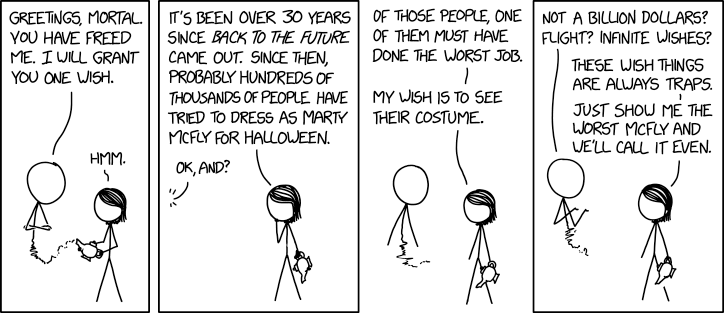
\includegraphics[width=\linewidth]{./images/well_ordering_principle.png}
\end{image}%
\tcblower
\end{figureptx}%
\footnotetext[3]{\nolinkurl{https://www.xkcd.com/2193/}\label{g:fn:idp105544811516688}}%
\begin{definition}{}{x:definition:def_integers}%
\index{integers}\index{\(\Z\)} The set of integers consists of the positive and negative natural numbers, together with zero, and is denoted by \(\Z\):%
\begin{equation*}
\Z = \set{\ldots, -3, -2, -1, 0, 1, 2, 3, \ldots}\text{.}
\end{equation*}
%
\end{definition}
\begin{assemblage}{Mathematical Induction.}{x:assemblage:induction}%
Let \(P(m)\) be a statement about the natural number \(m\)\footnotemark{}. Let \(k_0\in \N\) be such that the statement \(P(k_0)\) is true (the \emph{base case}), and suppose there is an \(n\ge k_0\) such that for all \(k\) satisfying \(k_0 \le k \le n\), \(P(k)\) is true (the \emph{inductive hypothesis}). Then \(P(n+1)\) is true, and thus \(P(m)\) is true for all \(m\ge k_0\) (the \emph{inductive step}).%
\end{assemblage}
\footnotetext[4]{Sample statements could include ``\(m\) is really interesting'' or ``\(3m^2 + m + 2\) is even''.\label{g:fn:idp105544811521552}}%
Mathematical induction is like climbing an infinite staircase. The \emph{base case} tells us that we can take a first step on the staircase (\(k_0\)). In the \emph{inductive hypothesis}, we assume we can take all the steps up to a certain height (\(n\)). In the \emph{inductive step}, we prove that this allows us to take the \((n+1)\)st step.%
\par
Thus, if we can take step \(k_0\), we can (by the inductive step) take step \(k_0 + 1\). And since we can take step \(k_0 + 1\), we can (again by the inductive step) take step \(k_0 + 2\). And so on, forever (or, if the notion of actual infinity makes you uncomfortable, as far as we want to go).%
\begin{assemblage}{Example.}{g:assemblage:idp105544811532432}%
For all \(n \ge 1\),%
\begin{equation*}
1+ 2 + 3 + \cdots + n = \frac{n(n+1)}{2}\text{.}
\end{equation*}
%
\par
\emph{Proof.} Base case: When \(n = 1\), the equation \(1 = \frac{1\cdot (1+1)}{2}\) is true.%
\par
\emph{Inductive Hypothesis:} Assume that there exists a \(n\) such that whenever \(k \le n\), the equation%
\begin{equation}
1+ 2 + 3 + \cdots + k = \frac{k(k+1)}{2}\label{x:men:ex_indhyp}
\end{equation}
is true.%
\par
\emph{Inductive Step:} Our goal is to show that \(P(n+1)\) is true. That is, we wish to establish that%
\begin{equation}
1+ 2 + 3 + \cdots + n + (n+1) = \frac{(n+1)((n+1)+1)}{2}\text{.}\label{x:men:ex_indgoal}
\end{equation}
%
\par
We begin on the left-hand side of \hyperref[x:men:ex_indhyp]{({\xreffont\ref{x:men:ex_indhyp}})}, where we may apply the inductive hypothesis to see that%
\begin{equation}
1+ 2 + 3 + \cdots + n + (n+1) = \left[\frac{n(n+1)}{2}\right] + (n+1)\text{.}\label{x:men:ex_indstep1}
\end{equation}
Through the use of straightforward algebra, the right-hand side becomes%
\begin{equation}
\frac{n(n+1)}{2} + \frac{2(n+1)}{2} = \frac{n(n+1) + 2(n+1)}{2} = \frac{(n+1)(n+2)}{2}\text{.}\label{x:men:ex_indstep2}
\end{equation}
%
\par
Putting \hyperref[x:men:ex_indstep1]{({\xreffont\ref{x:men:ex_indstep1}})} and \hyperref[x:men:ex_indstep2]{({\xreffont\ref{x:men:ex_indstep2}})} together, we obtain%
\begin{equation*}
1+ 2 + 3 + \cdots + n + (n+1) = \frac{(n+1)((n+1)+1)}{2}\text{,}
\end{equation*}
which is exactly the goal we stated in \hyperref[x:men:ex_indgoal]{({\xreffont\ref{x:men:ex_indgoal}})}.%
\end{assemblage}
We conclude with opportunities to practice induction.%
\begin{theorem}{}{}{g:theorem:idp105544811476880}%
For all \(k\ge 1\), \(3^k > k\).%
\end{theorem}
\begin{proof}{}{g:proof:idp105544811478160}
The statement is obviously true when \(k=1\).%
\par
Now suppose that \(k > 1\) and \(3^k > k\). Then \(3^{k+1} = 3\cdot 3^k > 3k = 2k + k > k+1\).%
\end{proof}
\begin{theorem}{}{}{g:theorem:idp105544811480336}%
Prove that the sum of the first \(n\) cubes is \(\dfrac{n^2(n+1)^2}{4}\). That is,%
%
\begin{equation*}
1^3 + 2^3 + 3^3 + \cdots + n^3 = \dfrac{n^2(n+1)^2}{4}.
\end{equation*}
\end{theorem}
\begin{proof}{}{g:proof:idp105544811482000}
We wish to prove that%
\begin{equation*}
1^3 + 2^3 + 3^3 + \cdots + n^3 = \frac{n^2(n+1)^2}{4}.
\end{equation*}
%
\par
\emph{Base Case:} When \(n=1\), the theorem clearly holds.%
\par
\emph{Inductive Hypothesis:} Assume for all \(k\le n\) that we have%
\begin{equation}
1^3 + 2^3 + 3^3 + \cdots + k^3 = \frac{k^2(k+1)^2}{4}.\label{x:men:eq-sum-of-cubes-ind-hyp}
\end{equation}
%
\par
\emph{Inductive Step:} We wish to prove that%
\begin{equation*}
1^3 + 2^3 + 3^3 + \cdots + n^3 +(n+1)^3 = \frac{(n+1)^2((n+1)+1)^2}{4} = \frac{(n+1)^2(n+2)^2}{4}.
\end{equation*}
We apply \hyperref[x:men:eq-sum-of-cubes-ind-hyp]{({\xreffont\ref{x:men:eq-sum-of-cubes-ind-hyp}})} to obtain%
\begin{align*}
1^3 + 2^3 + 3^3 + \cdots + n^3 +(n+1)^3 \amp = \frac{n^2(n+1)^2}{4} + (n+1)^3 \\
\amp = \frac{n^2(n+1)^2}{4} + \frac{4(n+1)^3}{4}\\
\amp = \frac{n^2(n+1)^2 + 4(n+1)^3}{4}\\
\amp = \frac{(n+1)^2 (n^2+4(n+1))}{4}\\
\amp = \frac{(n+1)^2 (n^2+4n+4)}{4}\\
\amp = \frac{(n+1)^2 (n+2)^2}{4}.
\end{align*}
The theorem is proved.%
\end{proof}
\begin{theorem}{(Bernoulli's Inequality).}{}{g:theorem:idp105544811488528}%
Given a real number \(b > -1\), \((1+b)^n \ge 1 + bn\) for all \(n\in \N_0\).\end{theorem}
\begin{proof}{}{g:proof:idp105544811490320}
When \(n=0\) the inequality becomes \(1 \ge 1\), which is clearly true.%
\par
Assume \(n > 0\). Then \((1+b)^{n+1} = (1+b)(1+b)^{n+1} \ge (1+b)(1+bn) = 1 +bn + b+b^2 n = 1 + b(n+1) + b^2 n	\ge 1+b(n+1)\).%
\end{proof}
\end{sectionptx}
%
%
\typeout{************************************************}
\typeout{Section 1.2 Divisibility and GCDs in the Integers}
\typeout{************************************************}
%
\begin{sectionptx}{Divisibility and GCDs in the Integers}{}{Divisibility and GCDs in the Integers}{}{}{x:section:SubSec-Divisibility-in-the-Integers}
\begin{assemblage}{Guiding Questions.}{g:assemblage:idp105544811493520}%
In this section, we'll seek to answer the questions: %
\begin{itemize}[label=\textbullet]
\item{}What does it mean for one integer to divide another?%
\item{}What properties does divisibility enjoy in the integers?%
\item{}What is the greatest common divisor of two integers?%
\item{}How can we compute the greatest common divisor of two integers?%
\end{itemize}
%
\end{assemblage}
%
%
\typeout{************************************************}
\typeout{Subsection 1.2.1 Divisibility and the Division Algorithm}
\typeout{************************************************}
%
\begin{subsectionptx}{Divisibility and the Division Algorithm}{}{Divisibility and the Division Algorithm}{}{}{g:subsection:idp105544811495696}
In this section, we begin to explore some of the arithmetic and algebraic properties of \(\Z\). We focus specifically on the divisibility and factorization properties of the integers, as these are the main focus of the text as a whole. One of the primary goals of this section is to formalize definitions that you are likely already familiar with and of which you have an intuitive understanding. At first, this might seem to unnecessarily complicate matters. However, it will become clear as we move forward that formal mathematical language and notation are necessary to extend these properties to a more abstract setting. We begin with a familiar notion.%
\begin{definition}{}{g:definition:idp105544811497104}%
\index{divides (integers)}%
\index{factor (integers)}%
Let \(a,b\in \Z\). We say that \(a\) \terminology{divides} \(b\), and write \(a\mid b\), if there is an integer \(c\) such that \(ac = b\). In this case, say that \(a\) and \(c\) are \terminology{factors} of \(b\). If no such \(c\in \Z\) exists, we write \(a\nmid b\).%
\end{definition}
Note that the symbol \(|\) is a \emph{verb}; it is therefore correct to say, e.g., \(2|4\), as 2 \emph{does} divide 4. However, it is an abuse of notation to say that \(2\mid 4 = 2\). Instead, we likely mean \(4\div 2 = 2\) or \(\frac{4}{2} = 2\) (though we will not deal in fractions just yet).%
\begin{investigation}{}{g:investigation:idp105544812095888}%
Determine whether \(a\mid b\) if:%
\begin{enumerate}
\item{}\(a = 3\), \(b = -15\)%
\item{}\(a = 4\), \(b = 18\)%
\item{}\(a = -7\), \(b = 0\)%
\item{}\(a = 0\), \(b = 0\)%
\end{enumerate}
Comment briefly on the results of this investigation. What did you notice? What do you still wonder?%
\par\smallskip%
\noindent\textbf{\blocktitlefont Solution}.\hypertarget{g:solution:idp105544812102928}{}\quad{}TBD.%
\end{investigation}%
We next collect several standard results about divisibility in \(\Z\) which will be used extensively in the remainder of this text.%
\begin{theorem}{}{}{g:theorem:idp105544812103952}%
Let \(a,b,c\in\Z\). If \(a\mid b\) and \(a\mid c\), then \(a\mid (b+c)\).%
\end{theorem}
\begin{proof}{}{g:proof:idp105544812106000}
Our hypothesis means that there exist integers \(k_1\) and \(k_2\) such that \(b = a k_1\) and \(c = a k_2\). Then \(b+c = a k_1 + a k_2 = a(k_1 + k_2)\). Let \(k' = k_1 + k_2\), and observe that \(k'\) is an integer; then \(b+c = a k'\), so \(a\mid (b+c)\).%
\end{proof}
\begin{theorem}{}{}{x:theorem:thm-divideproduct}%
Let \(a,b,c\in\Z\). If \(a\mid b\), then \(a\mid bc\).%
\end{theorem}
\begin{proof}{}{g:proof:idp105544812111632}
Our hypotheses means there is an integer \(k\) for which \(b = ak\). Then \(bc = (ak)c = a(kc)\). We observe that \(k' = kc\) is an integer, so \(bc = ak'\), and therefore \(a\mid bc\).%
\end{proof}
\begin{investigation}{}{x:investigation:invest-divideproduct}%
Consider the following partial converse to \hyperref[x:theorem:thm-divideproduct]{Theorem~{\xreffont\ref{x:theorem:thm-divideproduct}}}: If \(a,b,c\in\Z\) with \(a|bc\), must \(a|b\) or \(a|c\)? Supply a proof or give a counterexample.%
\par\smallskip%
\noindent\textbf{\blocktitlefont Solution}.\hypertarget{g:solution:idp105544812117136}{}\quad{}The converse is false: \(6| 3\cdot 4\), but \(6\nmid 3\) and \(6\nmid 4\).%
\end{investigation}%
\begin{theorem}{}{}{x:theorem:theorem_23lemmageneralization}%
Let \(a,b,c,d\in \Z\). If \(a = b+c\) and \(d\) divides any two of \(a,b,c\), then \(d\) divides the third.%
\end{theorem}
\begin{proof}{}{g:proof:idp105544812121232}
We consider two cases.%
\par
\emph{Case 1:} Assume without loss of generality that \(d|a\) and \(d|b\). Then there are integers \(k_1, k_2\) such that \(d k_1 = a\) and \(d k_2 = b\). We observe that \(c = a - b = d k_1 - d k_2 = d(k_1 - k_2)\), so \(d|c\).%
\par
\emph{Case 2:} Assume that \(d| b\) and \(d|c\), so there are \(k_1,k_2\in \Z\) such that \(d k_1 = b\) and \(d k_2 = c\). Then \(a = b+ c = dk_1 + dk_2 = d(k_1 + k_2)\), so \(d|a\).%
\end{proof}
\begin{investigation}{}{g:investigation:idp105544812062736}%
Formulate a conjecture akin to the previous theorems about divisibility in \(\Z\), and then prove it.%
\par\smallskip%
\noindent\textbf{\blocktitlefont Solution}.\hypertarget{g:solution:idp105544812063888}{}\quad{}Answers vary.%
\end{investigation}%
As we saw above, not all pairs of integers \(a,b\) satisfy \(a\mid b\) or \(b\mid a\). However, \href{http://www.corestandards.org/Math/Content/4/NBT/B/6/}{our experience in elementary mathematics does apply: there is often something left over (a remainder)}\footnote{\nolinkurl{http://www.corestandards.org/Math/Content/4/NBT/B/6/}\label{g:fn:idp105544812066064}}. The following theorem formalizes this idea for \(a,b\in \N\).%
\begin{theorem}{The Division Algorithm for \(\N\).}{}{x:theorem:thm_divalg}%
\index{Division Algorithm (\(\N\))}%
Let \(a,b\in \N\). Then there exist unique integers \(q,r\) such that \(a = bq + r\), where \(0 \le r \lt b\).%
\par\smallskip%
\noindent\textbf{\blocktitlefont 1.}\quad{}There are two parts to this theorem. First, you must establish that \(q\) and \(r\) exist. This is best done via \hyperref[x:axiom:axiom_wellordering]{Axiom~{\xreffont\ref{x:axiom:axiom_wellordering}}}. If you're stuck on that, check the second hint.%
\par
Once you have established that \(q\) and \(r\) exist, show that they are unique but assuming \(a = bq+r\) and \(a = bq' + r'\), where \(r,r'\) both satisfy the conditions of the theorem. Argue that \(q = q'\) and \(r = r'\).%
\par\smallskip%
\noindent\textbf{\blocktitlefont 2.}\quad{}Let \(S = \setof{a-bs}{s\in \N_0, a-bs\ge 0}\).%
\end{theorem}
\begin{proof}{}{g:proof:idp105544812075408}
First, assume that \(a \lt b\). Then \(q = 0\) and \(r = a\) are sufficient. If \(a = b\), then \(q = 1\) and \(r = 0\) will work.%
\par
Now, assume that \(a > b\). Then the set \(S = \setof{s\in\N}{a-bs \ge 0}\) is nonempty, as \(a-b\in S\). By \hyperref[x:axiom:axiom_wellordering]{Axiom~{\xreffont\ref{x:axiom:axiom_wellordering}}}, \(S\) has a least element, which we will call \(r\). Let \(q\in \N_0\) be such that \(r = a-bq\); then \(a = bq + r\).%
\par
To finish the proof, it is enough to show that this choice of \(r\) satisfies \(0\le r \le b-1\). Observe that \(r\in S\), so \(r\ge 0\). If \(r \ge b\), then \(a - b(q+1) = a-bq -b = r -b \ge 0\). Since \(q+1 > q\), this is a contradiction to the assumption that \(q\) was the largest element of \(S\). Thus, \(r \lt b\), i.e., \(r \le b-1\).%
\par
Let \(q,q',r,r'\) be such that \(a = bq+r\) and \(a=bq'+r'\). We see that \(bq+r = bq' + r'\), so \(b(q-q') = r'-r\), so \(b|r'-r\). If \(r'-r = 0\), we are done.%
\par
Otherwise, \(r'-r\) is a nonzero multiple of \(n\). If \(r' \ge r\), then \(0\le b(q-q') = r' - r \le b-1 - r\), a contradiction. Similarly, if \(r' \le r\), write \(b(q'-q) = r-r' \ge 0\), and a symmetric argument leads to a contradiction.%
\par
Thus, \(r' = r\), so \(b(q-q') = 0\), and since \(b > 0\), \(q - q'= 0\), i.e., \(q = q'\).%
\end{proof}
\begin{aside}{Warning!}{g:aside:idp105544812159504}%
This theorem has two parts: existence and uniqueness. Do not try to prove them both at the same time.%
\end{aside}
Unsurprisingly, the Division Algorithm also holds in \(\Z\), though the existence of negative integers requires a careful restatement. %
\begin{corollary}{The Division Algorithm for \(\Z\).}{}{g:corollary:idp105544812161168}%
\index{Division Algorithm (\(\Z\))}%
Let \(a,b\in \Z\) with \(b\ne 0\). Then there exist unique integers \(q,r\) such that \(a = bq + r\), where \(0 \le r \lt |b|\).%
\par\smallskip%
\noindentConsider cases, and apply \hyperref[x:theorem:thm_divalg]{Theorem~{\xreffont\ref{x:theorem:thm_divalg}}} wherever possible.%
\end{corollary}
\begin{proof}{}{g:proof:idp105544812165520}
TBD.%
\end{proof}
\end{subsectionptx}
%
%
\typeout{************************************************}
\typeout{Subsection 1.2.2 Greatest Common Divisors}
\typeout{************************************************}
%
\begin{subsectionptx}{Greatest Common Divisors}{}{Greatest Common Divisors}{}{}{g:subsection:idp105544812165904}
We next turn to another familiar property of the integers: the existence of greatest common divisors.%
\begin{definition}{}{x:definition:gcd-definition}%
\index{greatest common divisor (\(\Z\))}%
Let \(a,b\in \Z\) such that \(a\) and \(b\) are not both 0. A \terminology{greatest common divisor} of \(a\) and \(b\), denoted \(\gcd(a,b)\), is a natural number \(d\) satisfying%
\begin{enumerate}
\item{}\(d\mid a\) and \(d\mid b\)%
\item{}if \(e\in \N\) and \(e\mid a\) and \(e\mid b\), then \(e\mid d\).%
\end{enumerate}
%
\par
If \(\gcd(a,b) = 1\), we say that \(a\) and \(b\) are \terminology{relatively prime} or \terminology{coprime}. \begin{aside}{}{g:aside:idp105544812177296}%
\end{aside}
%
\end{definition}
\footnotetext[2]{\nolinkurl{http://www.corestandards.org/Math/Content/6/NS/B/4/}\label{g:fn:idp105544812177936}}%
This definition may be different than the one you are used to, which likely stated that \(d \ge e\) rather than condition 2 in \hyperref[x:definition:gcd-definition]{Definition~{\xreffont\ref{x:definition:gcd-definition}}}. It can be proved using the order relations of \(\Z\) that the definition given here is equivalent to that one. However, we will prefer this definition, as it generalizes naturally to other number systems which do not have an order relation like \(\Z\).%
\begin{activity}{}{x:activity:act-gcdcomputations}%
Compute \(\gcd(a,b)\) if:%
\begin{enumerate}
\item{}\(a = 123\), \(b = 141\)%
\item{}\(a = 0\), \(b = 169\)%
\item{}\(a= 85\), \(b = 48\)%
\end{enumerate}
Now that you have had a bit of practice computing gcds, describe your method for finding them in a sentence or two.%
\par\smallskip%
\noindent\textbf{\blocktitlefont Solution}.\hypertarget{g:solution:idp105544812186000}{}\quad{}TBD.%
\end{activity}%
How did you answer the last question in \hyperref[x:activity:act-gcdcomputations]{Activity~{\xreffont\ref{x:activity:act-gcdcomputations}}}? If you are like the authors' classes, the answers probably varied, though you have referred at some point to a "prime" (\hyperref[x:definition:def-primeinteger]{whatever those are}), or possibly some other ad hoc method for finding the gcd. Most such methods rely in some form on our ability to factor integers. However, the problem of factoring arbitrary integers is actually surprisingly computationally intensive. Thankfully, there is another way to compute \(\gcd(a,b)\), to which we now turn.%
\begin{theorem}{}{}{g:theorem:idp105544812188176}%
Let \(a,b,c\in\Z\) such that \(a = b+c\) with \(a\) and \(b\) not both zero. Then \(\gcd(a,b) = \gcd(b,c)\).%
\end{theorem}
\begin{proof}{}{g:proof:idp105544812125072}
Let \(d = \gcd(a,b)\) and \(e = \gcd(b,c)\). Since \(d|a\) and \(d|b\), \(d|c\), and so \(d|e\) by definition.%
\par
Similarly, since \(e|b\) and \(e|c\), \(e|a\), so \(e|d\) by definition.%
\par
Thus, \(e = d\).%
\end{proof}
\begin{investigation}{}{x:investigation:invest_gcdremainder}%
Suppose \(a,b,c\in\Z\) such that there exists \(q\in\Z\) with \(a = bq + c\) and \(a\) and \(b\) not both zero. Prove or disprove: \(\gcd(a,b)=\gcd(b,c)\).%
\par\smallskip%
\noindent\textbf{\blocktitlefont Solution}.\hypertarget{g:solution:idp105544812133392}{}\quad{}TBD.\end{investigation}%
\begin{investigation}{(Euclidean Algorithm).}{x:investigation:invest-euclid-alg-integers}%
\index{Euclidean Algorithm}%
Let \(a,b\in \N\). Use \hyperref[x:theorem:thm_divalg]{Theorem~{\xreffont\ref{x:theorem:thm_divalg}}} and \hyperref[x:investigation:invest_gcdremainder]{Investigation~{\xreffont\ref{x:investigation:invest_gcdremainder}}} to determine an algorithm for computing \(\gcd(a,b)\). How could your method be modified to compute \(\gcd(a,b)\) for \(a,b\in\Z\)?%
\par\smallskip%
\noindent\textbf{\blocktitlefont Solution}.\hypertarget{g:solution:idp105544812137616}{}\quad{}Let \(a,b\in \N\). Write \(a = bq_1+r_1\). By \hyperref[x:investigation:invest_gcdremainder]{Theorem~{\xreffont\ref{x:investigation:invest_gcdremainder}}}, \(\gcd(a,b) = \gcd(b,r_1)\).%
\par
Then, write \(b = r_1 q_2 + r_2\) using the Division algorithm. Observe \(\gcd(b,r_1) = \gcd(r_1,r_2)\). Continue until there is a \(k\) for which \(r_k = 0\), so \(\gcd(r_k,r_{k-1}) = r_{k-1}\). Then \(r_{k-1}= \gcd(r_k, r_{k-1}) = \gcd(r_{k-1},r_{k-2}) = \cdots = \gcd(a,b)\).%
\end{investigation}%
\begin{activity}{}{g:activity:idp105544812142224}%
Use the Euclidean algorithm to compute \(\gcd(18489,17304)\).%
\par\smallskip%
\noindent\textbf{\blocktitlefont Solution}.\hypertarget{g:solution:idp105544812143376}{}\quad{}We write%
\begin{align*}
18489 \amp = 17304 \cdot 1 +1185\\
17304 \amp = 1185\cdot 14 +714\\
1185 \amp = 714 \cdot 1 + 471\\
714 \amp = 471 \cdot 1+ 243\\
471 \amp = 243\cdot 1 + 228\\
243 \amp = 228 \cdot 1+ 15\\
228 \amp = 15 \cdot 15 + 3\\
15 \amp = 3\cdot 5 + 0\text{.}
\end{align*}
%
\par
So \(\gcd(18489,17304)=3\).%
\end{activity}%
The following identity provides a useful characterization of the greatest common divisor of two integers, not both zero. We will return to this idea several times, even after we have left the familiar realm of the integers.%
\begin{theorem}{Bézout's Identity.}{}{x:theorem:theorem_bezoutint}%
\index{Bézout's Identity}%
For any integers \(a\) and \(b\) not both 0, there are integers \(x\) and \(y\) such that%
\begin{equation*}
ax + by = \gcd(a,b)\text{.}
\end{equation*}
%
\par\smallskip%
\noindent\textbf{\blocktitlefont 1.}\quad{}Apply \hyperref[x:axiom:axiom_wellordering]{Axiom~{\xreffont\ref{x:axiom:axiom_wellordering}}} to a well-chosen set.%
\par\smallskip%
\noindent\textbf{\blocktitlefont 2.}\quad{}Apply \hyperref[x:axiom:axiom_wellordering]{Axiom~{\xreffont\ref{x:axiom:axiom_wellordering}}} to \(S = \setof{as+bt}{s,t\in\Z, \ as+bt \gt 0}\).%
\end{theorem}
\begin{proof}{}{g:proof:idp105544812151952}
Consider the set \(S = \setof{as+bt}{s,t\in\Z, \ as+bt \gt 0}\). We first show that \(S\ne \emptyset\).%
\par
Suppose without loss of generality that \(a\ne 0\), and consider \(a \gt 0\); then \(s=1, t = 0\) is sufficient to guarantee \(as+bt\in S\). If \(a \lt 0\), then \(s = -1, t= 0\) is sufficient. Regardless, \(S\ne \emptyset\), and by the Well-Ordering Principle, \(S\) has a least element, \(d = ax+by\). We claim \(d = \gcd(a,b)\).%
\par
We first show that \(d|a\) Use the division algorithm to write \(a = dq + r\), where \(r \lt d\). We find \(r = a - dq = a - (ax+by)q = a(1-xq) + by\), and if \(r\gt 0\), \(r\in S\), contradicting the status of \(d\) as the least element of \(S\). Thus, \(r = 0\), and \(d|a\). By a symmetric proof, \(d|b\).%
\par
Suppose then that \(e\) is a common divisor of \(a\) and \(b\); write \(a = e k_1\) and \(b = e k_2\). Then \(d = ax + by = (ek_1)x + (ek_2)y = e(k_1x + k_2 y)\), whence \(e|d\). Therefore, \(d = \gcd(a,b)\).%
\end{proof}
We conclude with an answer to the questions raised by \hyperref[x:investigation:invest-divideproduct]{Investigation~{\xreffont\ref{x:investigation:invest-divideproduct}}}.%
\begin{theorem}{}{}{x:theorem:theorem_relprimecancel}%
Let \(a, b\), and \(c\) be integers. If \(a|bc\) and \(\gcd(a,b) = 1\), then \(a|c\).%
\end{theorem}
\begin{proof}{}{g:proof:idp105544812233744}
Suppose \(\gcd(a,b) = 1\). By \hyperref[x:theorem:theorem_bezoutint]{Theorem~{\xreffont\ref{x:theorem:theorem_bezoutint}}}, there are integers \(x\) and \(y\) such that%
\begin{equation*}
ax+by = 1\text{.}
\end{equation*}
%
\par
Multiply by \(c\) to get%
\begin{equation*}
acx + bcy = c\text{.}
\end{equation*}
%
\par
Since \(a|bc\) by assumption, there is an integer \(k\) such that \(ak = bc\), so we have%
\begin{equation*}
acx + bcy = acx + aky = a(cx+ky) = c\text{,}
\end{equation*}
so \(a|c\).%
\end{proof}
\end{subsectionptx}
\begin{conclusion}{}%
In this section, we have collected some initial results about divisibility in the integers. We'll next explore the multiplicative building blocks of the integers, the primes, in preparation for a deeper exploration of factorization.%
\end{conclusion}%
\end{sectionptx}
%
%
\typeout{************************************************}
\typeout{Section 1.3 Primes and Factorization}
\typeout{************************************************}
%
\begin{sectionptx}{Primes and Factorization}{}{Primes and Factorization}{}{}{x:section:SubSec-Primes-and-Factorization}
\begin{assemblage}{Guiding Questions.}{g:assemblage:idp105544812240656}%
In this section, we'll seek to answer the questions: %
\begin{itemize}[label=\textbullet]
\item{}What are primes? What properties do they have?%
\item{}What does the Fundamental Theorem of Arithmetic say?%
\item{}Why is the Fundamental Theorem of Arithmetic true?%
\end{itemize}
%
\end{assemblage}
As described in the \hyperref[x:preface:Sec-Introduction]{Introduction}, our main goal is to build a deep structural understanding of the notion of \emph{factorization}. That is, splitting objects (e.g., numbers, polynomials, matrices) into products of other objects. One of the most familiar examples of this process involves factoring integers into products of primes.%
\begin{definition}{}{x:definition:def-primeinteger}%
\index{prime (integers)}%
\index{composite (integers)}%
Let \(p > 1\) be a natural number. We say \(p\) is \terminology{prime} if whenever \(a,b\in \Z\) such that \(p\mid ab\), either \(p\mid a\) or \(p\mid b\).%
\par
A natural number \(m > 1\) is said to be \terminology{composite} if it is not prime.%
\end{definition}
This is almost certainly not the definition of prime that you are familiar with from your school days, which likely said something to the effect that a prime \(p > 1\) is a natural number only divisible by 1 and itself. However, \hyperref[x:definition:def-primeinteger]{Definition~{\xreffont\ref{x:definition:def-primeinteger}}} is often more useful than the usual definition. And, as \hyperref[x:lemma:theorem_euclidslemma]{Lemma~{\xreffont\ref{x:lemma:theorem_euclidslemma}}} demonstrates, the two notions are equivalent.%
\begin{lemma}{Euclid's Lemma.}{}{x:lemma:theorem_euclidslemma}%
Given any \(p\in \N\), \(p > 1\), \(p\) is prime if and only if whenever \(m\in \N\) divides \(p\), either \(m = p\) or \(m = 1\).%
\end{lemma}
\begin{proof}{}{g:proof:idp105544812253712}
Let \(p\) be prime and suppose \(m\in \N\) divides \(p\), so \(p = mk\) for some \(k\in \N\). By definition, \(p|m\) or \(p|k\). If \(p|m\), then \(pj = m\), so \(p = pjk\), and \(jk=1\), which means \(j=k=1\) and thus \(m=p\). If \(p|k\), then \(pj=k\), so \(p = mpj\), and \(mj=1\), so \(m = j = 1\).%
\par
Conversely, assume \(p\in \N\) has the property that whenever an integer \(m\) exists with \(m|p\), then \(m= p\) or \(m =1\). Suppose \(p|ab\), so there exists a \(k\in\N\) such that \(pk = ab\). Note that if \(\gcd(a,p) = d > 1\), then \(d|p\), and so \(d = p\), and then \(p|a\). If \(\gcd(a,p) = 1\), then by Bézout's Identity there are integers \(x\) and \(y\) such that \(ax + py = 1\), so we may multiply by \(b\) to obtain \(abx + pby = b\), whence \(p|b\).%
\end{proof}
\begin{exploration}{}{x:exploration:question_compositecharacterization}%
Using \hyperref[x:lemma:theorem_euclidslemma]{Lemma~{\xreffont\ref{x:lemma:theorem_euclidslemma}}} as a guide, give a biconditional characterization for composite numbers. That is, finish the sentence: ``A number \(m\in\N\) is composite if and only if ....''%
\par\smallskip%
\noindent\textbf{\blocktitlefont Answer}.\hypertarget{g:answer:idp105544812205072}{}\quad{}``A number \(m\in\N\) is composite if and only if there exist natural numbers \(a,b\ne 1\) such that \(m = ab\).''%
\end{exploration}%
\begin{remark}{}{g:remark:idp105544812206992}%
How does your definition treat the number 1? The primality of 1 has been the subject of much debate stretching back to the Greeks (most of whom did not consider 1 to be a number). Throughout history, mathematicians have at times viewed 1 as prime, and at other times, not prime. The main argument for the non-primality of 1 is that if 1 were taken to be prime, we would need to word theorems like the Fundamental Theorem of Arithmetic (below) in such a way that only prime factorizations not including 1 can be considered. For, if 1 is prime, we would have to consider, e.g., \(6 = 2\cdot 3 = 1\cdot 2 \cdot 3 = 1\cdot 1\cdot 2\cdot 3\) as three different factorizations of 6 into primes.%
\par
However, neither is 1 composite (your definition should rule this out in some way). Instead, we call 1 a \terminology{unit}, which we'll explore more fully in \hyperref[x:definition:def-unit]{Definition~{\xreffont\ref{x:definition:def-unit}}} and the following; consequently, the opposite of "prime" is not "composite", but "not prime".%
\end{remark}
\begin{theorem}{}{}{g:theorem:idp105544812208912}%
Let \(a\in \N\) such that \(a > 1\). Then there is a prime \(p\) such that \(p\mid a\).%
\end{theorem}
\begin{proof}{}{g:proof:idp105544812210960}
We proceed by mathematical induction. Note that when \(a = 2\), the statement holds.%
\par
Assume that there is a \(k\in\N\) such that for all \(a\le k\), the statement holds. Consider \(k+1\). If \(k+1\) is prime, we are done. If not, then \(k+1\) is composite, and by the answer to \hyperref[x:exploration:question_compositecharacterization]{Question~{\xreffont\ref{x:exploration:question_compositecharacterization}}}, there are integers \(a,b\ne 1\) such that \(k+1 = ab\). By induction, there is a prime \(p\) such that \(p|a\), so \(p|k+1\).%
\end{proof}
\begin{theorem}{}{}{g:theorem:idp105544812216336}%
Suppose \(p\) and \(q\) are primes with \(p|q\). Then \(p = q\).%
\end{theorem}
\begin{proof}{}{g:proof:idp105544812218384}
TBD.\end{proof}
Our first major theorem makes two claims: that positive integers greater than 1 \emph{can} be factored into products of primes, and that this factorization can happen in only one way. As the semester progresses, we will see other theorems like this one, and catch glimpses of other ways to think about the \emph{unique factorization property}.%
\begin{assemblage}{Fundamental Theorem of Arithmetic.}{x:assemblage:ftarith}%
Every natural number greater than 1 is either a prime number or it can be expressed as a finite product of prime numbers where the expression is unique up to the order of the factors.%
\end{assemblage}
The proof is broken into two parts: existence (\hyperref[x:theorem:theorem_FTAexistence]{Theorem~{\xreffont\ref{x:theorem:theorem_FTAexistence}}}) and uniqueness (\hyperref[x:theorem:theorem_FTAuniqueness]{Theorem~{\xreffont\ref{x:theorem:theorem_FTAuniqueness}}}).%
\begin{theorem}{Fundamental Theorem of Arithmetic\textendash{}Existence Part\footnotemark{}.}{}{x:theorem:theorem_FTAexistence}%
Every natural number \(n > 1\) is either a prime number or it can be expressed as a finite product of prime numbers. That is, for every natural number \(n > 1\), there exist primes \(p_1, p_2, \ldots,
p_m\) and natural numbers \(r_1, r_2, \ldots, r_m\) such that%
\begin{equation*}
n = p_1^{r_1} p_2^{r_2} \cdots p_m^{r_m}\text{.}
\end{equation*}
%
\par\smallskip%
\noindentInduction!%
\end{theorem}
\footnotetext[1]{This approach to the Fundamental Theorem of Arithmetic is adapted from~[{\xreffont 1.3.1}].\label{g:fn:idp105544812288144}}%
\begin{proof}{}{g:proof:idp105544812291728}
It is enough to show that, if \(n > 1\), we may write \(n = p_1 p_2 \cdots p_k\), where the \(p_i\)'s are not necessarily distinct primes. Then we can collect the common primes and write them with exponent notation.%
\par
Note that when \(n = 2\), there is such an expression, so let \(k > 2\) be the least positive integer that fails to be expressed as above. We note that \(k\) cannot be prime, or it could be expressed as above. Thus, by Theorem 2.1, there is a prime \(p\) such that \(k = p b\), where \(1 \lt p, b \lt k\). Since \(k\) was the least positive integer that cannot be factored as a product of primes, \(b\) has a prime factorization. But then so does \(k\), a contradiction.%
\end{proof}
\begin{lemma}{}{}{g:lemma:idp105544812296976}%
Let \(p\) and \(q_1, q_2,\ldots,
q_n\) all be primes and let \(k\) be a natural number such that \(pk = q_1 q_2 \ldots q_n\). Then \(p = q_i\) for some \(i\).%
\end{lemma}
\begin{proof}{}{g:proof:idp105544812299792}
We first state a claim that will be useful.%
\par
\emph{Claim 1:} If \(p,q\) are primes such that \(p|q\), then \(p = q\).%
\par
\emph{Proof of Claim 1:} Since \(p,
q > 1\) and both \(p\) and \(q\) are prime, \(p = q\) by the definition of primality. \(\checkmark\)%
\par
Now assume that \(pk = q_1 q_2 \cdots q_n = (q_1 q_2 \cdots q_{n-1}) q_n\). If \(p|q_n\), we're done by Claim 1. If not, the definition of a prime guarantees that \(p| q_1 q_2 \cdots q_{n-1}\). If \(p|q_{n-1}\), we're done by Claim 1. Otherwise, \(p|q_1 q_2 \cdots q_{n-2}\).%
\par
Repeating this process, we see that either \(p|q_i\) for some \(i > 2\), or \(p|q_1 q_2\). Now the definition of a prime guarantees that \(p|q_1\) or \(p|q_2\), in which case Claim 1 requires that \(p = q_1\) or \(p = q_2\).%
\end{proof}
\begin{theorem}{Fundamental Theorem of Arithmetic\textendash{}Uniqueness Part.}{}{x:theorem:theorem_FTAuniqueness}%
Let \(n\) be a natural number. Let \(\set{p_1,p_2,\ldots,p_m}\) and \(\set{q_1,q_2,\ldots,q_s}\) be sets of primes with \(p_i\ne p_j\) if \(i\ne j\) and \(q_i\ne q_j\) if \(i\ne j\). Let \(\set{r_1,r_2,\ldots,r_m}\) and \(\set{t_1,t_2,\ldots,t_s}\) be sets of natural numbers such that%
\begin{align*}
n \amp = p_1^{r_1} p_2^{r_2} \cdots p_m^{r_m}\\
\amp = q_1^{t_1} q_2^{t_2} \cdots q_s^{t_s}\text{.}
\end{align*}
%
\par
Then \(m = s\) and \(\set{p_1,p_2,\ldots,p_m} = \set{q_1,q_2,\ldots,q_s}\). That is, the sets of primes are equal but their elements are not necessarily listed in the same order (i.e., \(p_i\) may or may not equal \(q_i\)). Moreover, if \(p_i = q_j\), then \(r_i = t_j\). In other words, if we express the same natural number as a product of distinct primes, then the expressions are identical except for the ordering of the factors.%
\par\smallskip%
\noindentArgue that the two sets are equal (how do we do that?). Then argue that the exponents must also be equal.%
\end{theorem}
\begin{proof}{}{g:proof:idp105544812318096}
Without loss of generality, assume \(p_1 \lt  p_2 \lt  \cdots \lt  p_m\) and \(q_1 \lt  q_2 \lt  \cdots \lt  q_s\). Given a \(p_i\), we know that \(p_i | q_1^{t_1} q_2^{t_2} \cdots q_s^{t_s}\), which implies that \(p_i | q_j\) for some \(j\) by Claim 2 in the proof of Lemma 2.8. Further, Lemma 2.8 implies that \(p_i = q_j\), and similarly, given a \(q_j\), \(q_j = p_i\) for some \(i\). Thus, \(m =s\), and by the ordering of the \(p_i\)'s and \(q_j\)'s, we have \(p_i = q_j\), \(i = 1, 2, \ldots, m\). Therefore,%
\begin{equation*}
n = p_1^{r_1} p_2^{r_2} \cdots p_m^{r_m} = p_1^{t_1} p_2^{t_2} \cdots p_m^{t_m}\text{.}
\end{equation*}
%
\par
Now, assume by way of contradiction, that \(r_i \ne t_i\) for some \(i\). Without loss of generality, we may assume \(r_i \lt  t_i\). Then \(p_i^{t_i} | p_1^{r_1} p_2^{r_2} \cdots p_m^{r_m}\), which implies that%
\begin{equation*}
p_i^{t_i - r_i} | p_1^{r_1} p_2^{r_2} \cdots \hat{p}_i^{r_i} \cdots p_m^{r_m}\text{.}
\end{equation*}
%
\par
Since \(t_i - r_i > 0\), we have that%
\begin{equation*}
p_i  | p_1^{r_1} p_2^{r_2} \cdots \hat{p}_i^{r_i} \cdots p_m^{r_m}\text{,}
\end{equation*}
from which \(p_i | p_j\) for some \(j\ne i\) by Lemma 2.8. This is a contradiction, so \(r_i = t_i\) for \(i = 1, 2, \ldots, m\).%
\end{proof}
Our first major result is in hand: we can factor natural numbers \(n > 2\) uniquely as a product of primes. Much of the rest of this book seeks to deduce a generalization of this result that relies on structural arithmetic properties enjoyed by \(\Z\) and similar objects.%
%
%
\typeout{************************************************}
\typeout{References 1.3 References}
\typeout{************************************************}
%
\begin{references-subsection-numberless}{References}{}{References}{}{}{g:references:idp105544812264848}
D. Marshall, E. Odell, M. Starbird, \emph{Number Theory Through Inquiry}, MAA Textbooks, Mathematical Association of America, 2007\end{references-subsection-numberless}
\end{sectionptx}
%
%
\typeout{************************************************}
\typeout{Section 1.4 The Integers modulo \(m\)}
\typeout{************************************************}
%
\begin{sectionptx}{The Integers modulo \(m\)}{}{The Integers modulo \(m\)}{}{}{x:section:SubSec-Integers-Mod-m}
\begin{assemblage}{Guiding Questions.}{g:assemblage:idp105544812267280}%
In this section, we'll seek to answer the questions: %
\begin{itemize}[label=\textbullet]
\item{}What are equivalence relations?%
\item{}What is congruence modulo \(m\)?%
\item{}How does arithmetic in \(\Z_m\) compare to arithmetic in \(\Z\)?%
\end{itemize}
%
\end{assemblage}
The foundation for our exploration of abstract algebra is nearly complete. We need the basics of one more "number system" in order to appreciate the abstract approach developed in subsequent chapters. To build that number system, a brief review of relations and equivalence relations is required. Recall that given sets \(S\) and \(T\), the Cartesian product of \(S\) with \(T\), denoted \(S\times T\) ("\(S\) cross \(T\)"), is the set of all possible ordered pairs whose first element is from \(S\) and second element is from \(T\). Symbolically,%
%
\begin{equation*}
S\times T = \setof{(s,t)}{s\in S, \ t\in T}.
\end{equation*}
\begin{definition}{}{g:definition:idp105544812274320}%
\index{relation}%
Let \(S\) be a nonempty set. A \terminology{relation} \(R\) on \(S\) is a subset of \(S\times S\). If \(x,y\in S\) such that \((x,y)\in R\), we usually write \(xRy\) and say that \(x\) and \(y\) are \terminology{related under \(R\)}.%
\end{definition}
The notion of a relation as presented above is extremely open-ended. \emph{Any} subset of ordered pairs of \(S\times S\) describes a relation on the set \(S\). Of course, some relations are more meaningful than others; the branch of mathematics known as \href{https://en.wikipedia.org/wiki/Order_theory}{order theory}\footnote{\nolinkurl{https://en.wikipedia.org/wiki/Order_theory}\label{g:fn:idp105544812281360}} studies \emph{order} relations (such as the familiar \(\lt\)). Our focus will be on \emph{equivalence relations}, which isolate the important features of \(=\).%
\begin{definition}{}{x:definition:def-eqrel}%
\index{equivalence relation}%
\index{equivalence class}%
\index{equivalence class, representative of}%
Let \(S\) be a nonempty set. We say a relation \(\sim\) on \(S\) is an \terminology{equivalence relation} if the following properties hold:%
\begin{itemize}[label=\textbullet]
\item{}\(\sim\) is \emph{reflexive}: if \(a\in S\), then \(a\sim a\).%
\item{}\(\sim\) is \emph{symmetric}: if \(a,b\in S\) with \(a\sim b\), then \(b\sim a\).%
\item{}\(\sim\) is \emph{transitive}: if \(a,b,c\in S\) with \(a\sim b\) and \(b\sim c\), then \(a\sim c\).%
\end{itemize}
%
\par
Given \(x\in S\), the set%
\begin{equation*}
\overline{x} = \setof{y\in S}{x\sim y}
\end{equation*}
is called the \terminology{equivalence class of \(x\)}. Any element \(z\in \overline{x}\) is called a \terminology{representative} of the equivalence class.%
\end{definition}
\begin{activity}{}{g:activity:idp105544811837840}%
Prove that ``has the same birthday as'' is an equivalence relation on the set \(P\) of all people.%
\par\smallskip%
\noindent\textbf{\blocktitlefont Solution}.\hypertarget{g:solution:idp105544811839376}{}\quad{}Given any \(x\in P\), clearly \(x\) has the same birthday as \(x\).%
\par
Moreover, if \(x,y\in P\) such that \(x\) has the same birthday as \(y\), then it is clear that \(y\) has the same birthday as \(x\).%
\par
Finally, if \(x,y,z\in P\) such that \(x\) has the same birthday as \(y\) and \(y\) has the same birthday as \(z\), then \(x\) must have the same birthday as \(z\).%
\end{activity}%
\begin{exploration}{}{g:exploration:idp105544811846032}%
What other relations can you think of? Write down one example and one non-example of an equivalence relation.%
\end{exploration}%
\begin{activity}{}{g:activity:idp105544811846800}%
Prove that \(\le\) is \emph{not} an equivalence relation on \(\Z\).%
\par\smallskip%
\noindent\textbf{\blocktitlefont Solution}.\hypertarget{g:solution:idp105544811848720}{}\quad{}The relation \(\le\) fails the symmetry condition. As an example, note that \(2 \le 3\), but \(3\not\le 2\).%
\end{activity}%
For our purposes, a particularly important equivalence relation is congruence modulo \(m\) on the set of integers.%
\begin{definition}{}{g:definition:idp105544811850896}%
\index{congruence modulo \(m\)}%
Let \(a,b\in \Z\) and \(m \in \N\), \(m > 1\). We say \terminology{\(a\) is congruent to \(b\) modulo \(m\)} if \(m\mid a-b\). We write \(a \equiv b\mod m\).%
\end{definition}
\begin{activity}{}{g:activity:idp105544811855120}%
Justify the following congruences.%
\begin{enumerate}
\item{}\(\displaystyle 18 \equiv 6\mod 12\)%
\item{}\(\displaystyle 47 \equiv 8\mod 13\)%
\item{}\(\displaystyle 71 \equiv 1\mod 5\)%
\item{}\(\displaystyle 21 \equiv -1 \mod 11\)%
\item{}\(\displaystyle 24 \equiv 0\mod 6\)%
\end{enumerate}
%
\end{activity}%
\begin{theorem}{}{}{g:theorem:idp105544811858064}%
Given an integer \(m > 1\), congruence modulo \(m\) is an equivalence relation on \(\Z\).%
\end{theorem}
\begin{proof}{}{g:proof:idp105544811859728}
Let \(a\in \Z\). Then \(m|a-a\), so \(a \equiv_m a\). Thus, \(\equiv_m\) is reflexive.%
\par
Let \(a,b\in \Z\) such that \(a\equiv_m b\). This means that \(m|a-b\), so there is some \(k\in \Z\) such that \(mk = a-b\). Then \(m(-k) = b-a\), so \(m|b-a\) and \(b \equiv_m a\). Thus, \(\equiv_m\) is symmetric.%
\par
Finally, let \(a,b,c\in \Z\) such that \(a\equiv_m b\) and \(b\equiv_m c\). Then \(m|a-b\) and \(m|b-c\), so there are integers \(k_1, k_2\) such that \(m k_1 = a-b\) and \(m k_2 = b-c\). Summing these equations yields \(m(k_1 + k_2) = (a-b) + (b-c) = a-c\), so \(m|a-c\) and \(a\equiv_m c\).%
\end{proof}
\index{\(\Z_m\)} The set of equivalence classes of \(\Z\) under the equivalence relation \emph{congruence modulo \(m\)} is called \terminology{the integers modulo \(m\)}, and is denoted \(\Z_m\) (pronounced "Z mod m").%
\begin{exploration}{}{g:exploration:idp105544811807120}%
List the elements of \(\Z_5\) and \(\Z_7\).%
\par\smallskip%
\noindent\textbf{\blocktitlefont Answer}.\hypertarget{g:answer:idp105544811808656}{}\quad{}The equivalence classes of \(\Z_5\) are%
\begin{align*}
\overline{0} \amp = \setof{7k}{k\in\Z} = \set{\ldots, -5, 0, 5, 10, \ldots}\\
\overline{1} \amp = \setof{7k+1}{k\in\Z} = \set{\ldots, -4, 1, 6, 11, \ldots}\\
\overline{2} \amp = \setof{7k+2}{k\in\Z} = \set{\ldots, -3, 2, 7, 12, \ldots}\\
\overline{3} \amp = \setof{7k+3}{k\in\Z} = \set{\ldots, -2, 3, 8, 13, \ldots}\\
\overline{4} \amp = \setof{7k+4}{k\in\Z} = \set{\ldots, -1, 4, 9, 14, \ldots}
\end{align*}
Since every integer is in one of the above equivalence classes, we know we have found them all.%
\end{exploration}%
\begin{theorem}{}{}{x:theorem:thm-additionmodulom}%
Let \(a,b, c,d\in \Z\) and \(m > 1\) such that \(a\equiv c\mod m\) and \(b\equiv d\mod m\). Then \(a+b \equiv c + d \mod m\).%
\end{theorem}
\begin{proof}{}{g:proof:idp105544811813648}
Write \(mk_1 = a-c\) and \(m k_2 = b-d\) for some \(k_1,k_2\in \Z\). Then \(m(k_1 + k_2) = (a-c) + (b-d) = (a+b) - (c+d)\), so \(a+b \equiv c+d\mod m\).%
\end{proof}
\begin{theorem}{}{}{g:theorem:idp105544811815952}%
Let \(a,b, c,d\in \Z\) and \(m > 1\) such that \(a\equiv c\mod m\) and \(b\equiv d\mod m\). Then \(ab \equiv c d\mod m\).%
\end{theorem}
\begin{proof}{}{g:proof:idp105544811818384}
Write \(mk_1 = a-c\) and \(m k_2 = b-d\) for some \(k_1,k_2\in \Z\). Observe%
\begin{align*}
ab -cd \amp = ab - bc + bc - cd\\
\amp = b(a-c) + c(b-d)\\
\amp = bmk_1 + cmk_2\\
\amp = m(bk_1 + ck_2)\text{.}
\end{align*}
%
\par
Thus, \(m|ab-cd\) and \(ab \equiv cd\mod m\).%
\end{proof}
\begin{definition}{}{x:definition:def-well-defined}%
\index{well-defined statement}%
Let \(S\) be a set and \(\sim\) an equivalence relation on \(S\). Then a statement \(P\) about the equivalence classes of \(S\) is \terminology{well-defined} if the representative of the equivalence class does not matter. That is, whenever \(\overline{x} = \overline{y}\), \(P(\overline{x}) = P(\overline{y})\).%
\end{definition}
The previous exercises justify the following definitions.%
\begin{definition}{}{x:definition:def-arithemticmodm}%
Let \(m > 1\) and \(\overline{a},\overline{b}\in \Z_m\). Then the following are well-defined operations on the equivalence classes:%
\begin{enumerate}
\item{}\emph{Addition modulo \(m\)}: \(\overline{a} + \overline{b} := \overline{a+b}\). \begin{aside}{}{g:aside:idp105544811895056}%
\end{aside}
%
\item{}\emph{Multiplication modulo \(m\)}: \(\overline{a}\cdot \overline{b} := \overline{a\cdot b}\).%
\end{enumerate}
%
\end{definition}
Most elementary propositions about \(\Z_m\) can be recast as statements about \(\Z\). For instance, in proving \hyperref[x:theorem:thm-additionmodulom]{Theorem~{\xreffont\ref{x:theorem:thm-additionmodulom}}} you likely proved that if \(m|a-c\) and \(m|b-d\) that \(m|(a+b)-(c+d)\). However, as the statements become more complex, repeatedly reshaping statements about \(Z_m\) as statements about \(\Z\) becomes cumbersome and unhelpful. Instead, you are encouraged to become comfortable doing arithmetic modulo \(m\) or, put another way, arithmetic with the equivalence classes of \(\Z_m\) as defined in \hyperref[x:definition:def-arithemticmodm]{Definition~{\xreffont\ref{x:definition:def-arithemticmodm}}}.%
\begin{activity}{}{g:activity:idp105544811902736}%
Without passing back to \(\Z\), find the smallest nonnegative integer representative of the resulting equivalence classes.%
%
\begin{enumerate}
\item{}\(\overline{5}+\overline{11}\) in \(\Z_{9}\)%
\item{}\(\overline{-3}+\overline{-3}\) in \(\Z_{6}\)%
\item{}\(\overline{8}\cdot\overline{3}\) in \(\Z_{19}\)%
\item{}\(\overline{-1}\cdot(\overline{3}+\overline{8})\) in \(\Z_{7}\)%
\item{}\(\overline{3}\cdot(\overline{5}^2+\overline{3}^3)\) in \(\Z_{20}\)%
\end{enumerate}
\par\smallskip%
\noindent\textbf{\blocktitlefont Solution}.\hypertarget{g:solution:idp105544811907856}{}\quad{}TBD\end{activity}%
In the remainder of this section, we investigate fundamental properties of arithmetic in \(\Z_m\).%
\begin{investigation}{}{x:investigation:q_zmodmcancel}%
Let \(\overline{a},\overline{b},\overline{c}\in \Z_m\) with \(\overline{c}\ne\overline{0}\) and \(m > 1\). If \(\overline{a}\cdot \overline{c} = \overline{b}\cdot \overline{c}\), is it true that \(\overline{a} = \overline{b}\)? If so, prove it. If not, find an example of when the statement fails to hold.%
\par\smallskip%
\noindent\textbf{\blocktitlefont Answer}.\hypertarget{g:answer:idp105544811911568}{}\quad{}It is not true. For example, in \(\Z_{12}\), \(\overline{6}\cdot \overline{3} = \overline{6}\cdot\overline{1}\), but \(\overline{3}\ne \overline{1}\).%
\end{investigation}%
\begin{theorem}{}{}{x:theorem:theorem_cancelrelprime}%
Let \(a,b,c\), and \(m\) be integers with \(m > 1\) and \(\gcd(c,m)=1\). Then there is some \(x\in \Z\) such that \(\overline{c} \overline{x} = \overline{1}\).%
\par
Conclude that if \(\overline{a} \cdot\overline{c} = \overline{b}\cdot\overline{c}\) in \(\Z_m\) that \(\overline{a} = \overline{b}\).%
\end{theorem}
\begin{proof}{}{g:proof:idp105544811917456}
We know that \(m|ac-bc\), i.e., that \(m|c(a-b)\). By \hyperref[x:theorem:theorem_relprimecancel]{Theorem~{\xreffont\ref{x:theorem:theorem_relprimecancel}}}, \(m|a-b\).%
\end{proof}
\begin{theorem}{}{}{x:theorem:theorem_cancelinZp}%
Let \(p\in \N\) be prime and \(\overline{a},\overline{b},\overline{c}\in \Z_p\) such that \(\overline{c}\ne \overline{0}\). Then%
\begin{enumerate}
\item{}there is some \(\overline{x}\in \Z_p\) such that \(\overline{c}\cdot \overline{x} = \overline{1}\); and,%
\item{}if \(\overline{a} \cdot\overline{c} = \overline{b}\cdot\overline{c}\), \(\overline{a} = \overline{b}\).%
\end{enumerate}
%
\end{theorem}
\begin{proof}{}{g:proof:idp105544811924368}
In \(\Z_p\), every nonzero equivalence class is represented by an \(x\) for which \(\gcd(x,p) = 1\). Apply \hyperref[x:theorem:theorem_cancelrelprime]{Theorem~{\xreffont\ref{x:theorem:theorem_cancelrelprime}}}.%
\end{proof}
\end{sectionptx}
\end{chapterptx}
%
%
\typeout{************************************************}
\typeout{Chapter 2 Fields and Rings}
\typeout{************************************************}
%
\begin{chapterptx}{Fields and Rings}{}{Fields and Rings}{}{}{x:chapter:Sec-Fields-and-Rings}
\begin{introduction}{}%
You have been exploring numbers and the patterns they hide within them since your earliest school days. In Chapter 1 we reminded ourselves about some of those patterns (with the goal of understanding factorization) and worked to express them in a more formal way. You may find yourself wondering why we are going out of our way to complicate ideas you have understood since elementary school. The reason for the abstraction (and the reason for this course!) is so that we can explore just how far we can push these patterns. How far does our understanding of factorization in the integers stretch to other types of numbers and other mathematical objects (like polynomials)? In this chapter we will set the ground work for answering that question by introducing ideas that will assist us in streamlining our investigation into factorization.%
\end{introduction}%
%
%
\typeout{************************************************}
\typeout{Section 2.1 Fields}
\typeout{************************************************}
%
\begin{sectionptx}{Fields}{}{Fields}{}{}{x:section:SubSec-Fields}
\begin{assemblage}{Guiding Questions.}{g:assemblage:idp105544811862928}%
In this section, we'll seek to answer the questions: %
\begin{itemize}[label=\textbullet]
\item{}What are binary operations?%
\item{}What is a field? What sorts of things can one do in a field?%
\item{}What are examples of fields?%
\end{itemize}
%
\end{assemblage}
We now begin the process of abstraction. We will do this in stages, beginning with the concept of a \emph{field}. First, we need to formally define some familiar sets of numbers.%
\begin{definition}{}{g:definition:idp105544811865616}%
The rational numbers, denoted by \(\Q\), is the set%
\begin{equation*}
\Q = \setof{\frac{a}{b}}{a,b\in \Z, \ b\ne 0}\text{.}
\end{equation*}
%
\end{definition}
Recall that in elementary school, you learned that two fractions \(\frac{a}{b}, \frac{c}{d} \in \Q\) are equivalent if and only if \(ad=bc\).%
\begin{activity}{}{g:activity:idp105544811867920}%
Prove that our elementary school definition of equivalent fractions is an equivalence relation. Recall \hyperref[x:definition:def-eqrel]{Definition~{\xreffont\ref{x:definition:def-eqrel}}}.%
\end{activity}%
We likely have an intuitive idea of what is meant by \(\R\), the set of real numbers. Defining \(\R\) rigorously is actually quite difficult, and occupies a significant amount of time in a first course in real analysis. Thus, we will make use of your intuition. %
\par
Out of \(\R\) we may build the complex numbers.%
\begin{definition}{}{g:definition:idp105544811871120}%
The \terminology{complex numbers} consist of all expressions of the form \(a+bi\), where \(a,b\in \R\) and \(i^2 = -1\). Given \(z = a+bi\), we say \(a\) is the \terminology{real part} of \(z\) and \(b\) is the \terminology{imaginary part}. The set of complex numbers is denoted \(\C\).%
\end{definition}
As was mentioned in the \hyperref[x:preface:Sec-Introduction]{Introduction}, \emph{algebra} comes from an Arabic word meaning ``the reunion of broken parts''. We therefore need a way of combining two elements of a set into one; we turn to a particular type of function, known as a binary operation, to accomplish this.%
\begin{definition}{}{x:definition:def_binaryoperation}%
\index{binary operation}%
\index{binary operation} Let \(X\) be a nonempty set. A function \(\star : X \times X \to X\) is called a \terminology{binary operation}. If \(\star\) is a binary operation on \(X\), we say that \(X\) is \terminology{closed under the operation \(\star\)}. [Given \(a,b\in X\), we usually write \(a\star b\) in place of the typical function notation, \(\star(a,b)\).]%
\end{definition}
\begin{investigation}{}{x:investigation:invest-binop}%
Which of \(+, -, \cdot, \div\) are binary operations:%
\begin{enumerate}
\item{}on \(\R\)?%
\item{}on \(\Q\)?%
\item{}on \(\Z\)?%
\item{}on \(\N\)?%
\item{}on \(\C\)? (Recall that for \(a_1 + b_1 i, a_2 + b_2 i \in \C\), \((a_1 + b_1 i) + (a_2 + b_2 i) := (a_1 + a_2) + (b_1 + b_2)i\) and  \((a_1 + b_1 i)(a_2 + b_2 i) := (a_1 a_2 - b_1 b_2) + (a_1 b_2 + b_1 a_2) i\).)%
\end{enumerate}
%
\par\smallskip%
\noindent\textbf{\blocktitlefont Answer}.\hypertarget{g:answer:idp105544811890832}{}\quad{}Division is never a binary operation. The others are binary operations on \(\C\), \(\R, \Q\), and \(\Z\). The only binary operation on \(\N\) is addition.%
\end{investigation}%
\begin{activity}{}{g:activity:idp105544811892752}%
Choose your favorite nonempty set \(X\) and describe a binary operation different than those in \hyperref[x:investigation:invest-binop]{Investigation~{\xreffont\ref{x:investigation:invest-binop}}}.%
\par\smallskip%
\noindent\textbf{\blocktitlefont Answer}.\hypertarget{g:answer:idp105544811894288}{}\quad{}Answers vary, but one option is to define \(\min : \Z\times \Z \to \Z\) by%
%
\begin{equation*}
\min(a,b) := \begin{cases} a \amp \text{if } a \le b\\ b \amp \text{if } b\le a\end{cases.}
\end{equation*}
\end{activity}%
The hallmark of modern pure mathematics is the use of \emph{axioms}. An axiom is essentially an unproved assertion of truth. Our use of axioms serves several purposes.%
\par
From a logical perspective, axioms help us avoid the problem of infinite regression (e.g., asking \emph{How do you know?} over and over again). That is, axioms give us very clear starting points from which to make our deductions.%
\par
To that end, our first abstract algebraic structure captures and axiomatizes familiar behavior about how numbers can be combined to produce other numbers of the same type.%
\begin{definition}{}{x:definition:def_field}%
\index{field}%
A \terminology{field} is a nonempty set \(F\) with at least two elements and binary operations \(+\) and \(\cdot\), denoted \((F,+,\cdot)\), and satisfying the following \terminology{field axioms}:%
\begin{enumerate}
\item{}Given any \(a,b,c\in F\), \((a+b)+c = a+(b+c)\). (Associativity of addition)%
\item{}Given any \(a,b\in F\), \(a+b= b+a\). (Commutativity of addition)%
\item{}There exists an element \(0_F\in F\) such that for all \(a\in F\), \(a+0_F = 0_F + a = a\). (Additive identity)%
\item{}Given any \(a\in F\) there exists a \(b\in F\) such that \(a+b = b + a =0_F\). (Additive inverse)%
\item{}Given any \(a,b,c\in F\), \((a\cdot b)\cdot c = a\cdot (b\cdot c)\). (Associativity of multiplication)%
\item{}Given any \(a,b\in F\), \(a\cdot b = b\cdot a\). (Commutativity of multiplication)%
\item{}There exists an element \(1_F\in F\) such that for all \(a\in F\), \(1_F\cdot a = a\cdot 1_F = a\). (Multiplicative identity)%
\item{}For all \(a\in F\), \(a\ne 0_F\), there exists a \(b\in F\) such that \(a\cdot b = b\cdot a = 1_F\). (Multiplicative inverse)%
\item{}For all \(a,b,c\in F\), \(a\cdot (b+c) = a\cdot b + a\cdot c\). (Distributive property I)%
\item{}For all \(a,b,c\in F\), \((a+b)\cdot c = a\cdot c + b\cdot c\). (Distributive property II)%
\end{enumerate}
%
\end{definition}
We will usually write \(a\cdot b\) as \(ab\). Additionally, we will usually drop the subscripts on \(0,1\) unless we need to distinguish between fundamentally different identities in different fields.%
\begin{investigation}{}{x:investigation:exer_fieldexamples}%
Which of the following are fields under the specified operations? For most, a short justification or counterexample is sufficient.%
\begin{enumerate}
\item{}\(\N\) under the usual addition and multiplication operations%
\item{}\(\Z\) under the usual addition and multiplication operations%
\item{}\(2\Z\), the set of even integers, under the usual addition and multiplication operations%
\item{}\(\Q\) under the usual addition and multiplication operations%
\item{}\(\Z_{6}\) under addition and multiplication modulo 6%
\item{}\(\Z_{5}\) under addition and multiplication modulo 5%
\item{}\(\R\) under the usual addition and multiplication operations%
\item{}\(\C\) under the complex addition and multiplication defined in \hyperref[x:investigation:invest-binop]{Investigation~{\xreffont\ref{x:investigation:invest-binop}}}%
\item{}\(\mathcal{M}_2(\R) := \setof{\left(\begin{matrix}a \amp b \\ c \amp d \end{matrix} \right)}{a,b,c,d\in\R}\)\footnotemark{}, the set of \(2\times 2\) matrices with real coefficients using the usual definition of matrix multiplication\footnotemark{} and matrix addition.%
\end{enumerate}
%
\par\smallskip%
\noindent\textbf{\blocktitlefont Solution}.\hypertarget{g:solution:idp105544811930768}{}\quad{}%
\begin{enumerate}
\item{}\(\N\) is not closed under taking additive inverses, so is not a field.%
\item{}\(\Z\) is not a field, as there is no integer \(a\) such that \(2a = 1\).%
\item{}\(2\Z\) is not a field for the same reason.%
\item{}\(\Q\) is a field.%
\item{}\(\Z_{6}\) is not a field; there is no \(\overline{a}\in \Z_{10}\) for which \(\overline{2}\cdot \overline{a} = \overline{1}\) (you can check them all; there are only 4 viable options).%
\item{}\(\Z_{5}\) \emph{is} a field. The axioms pertaining to addition and multiplication were established earlier or rely on the same axioms holding for \(\Z\).%
\item{}\(\R\) is a field%
\item{}\(\C\) is a field. Given \(a+bi\ne 0\), \((a+bi)^{-1} = \frac{a}{a^2 + b^2} - \frac{b}{a^2 + b^2} i\).%
\item{}\(\mathcal{M}_2(\R)\) is not a field. Matrix multiplication is not commutative.%
\end{enumerate}
%
\end{investigation}%
\footnotetext[1]{For students who have taken a linear algebra course.\label{g:fn:idp105544811928592}}%
\footnotetext[2]{Recall that, if \(\left(\begin{matrix}a_1 \amp b_1 \\ c_1 \amp d_1 \end{matrix} \right), \left(\begin{matrix}a_2 \amp b_2 \\ c_2 \amp d_2 \end{matrix} \right)\in \mathcal{M}_2(\R)\), then \(\left(\begin{matrix}a_1 \amp b_1 \\ c_1 \amp d_1 \end{matrix} \right) \cdot \left(\begin{matrix}a_2 \amp b_2 \\ c_2 \amp d_2 \end{matrix} \right) = \left(\begin{matrix}a_1 a_2 + b_1 c_2 \amp a_1 b_2 + b_1 d_2 \\ c_1 a_2 + d_1 c_2 \amp c_1 b_2 + d_1 d_2 \end{matrix} \right)\).\label{g:fn:idp105544811929360}}%
In the \hyperref[x:investigation:exer_fieldexamples]{Investigation~{\xreffont\ref{x:investigation:exer_fieldexamples}}}, you determined which of sets of familiar mathematical objects are and are not fields. Notice that you have been working with fields for years and that our abstraction of language to that of fields is simply to allow us to explore the common features at the same time - it is inefficient to prove the same statement about every single field when we can prove it once and for all about fields in general.%
\begin{theorem}{Properties of Fields.}{}{x:theorem:thm_fieldproperties}%
Let \(F\) be a field.%
\begin{enumerate}
\item{}The additive identity \(0\) is unique.%
\item{}For all \(a\in F\), \(a \cdot 0 = 0\cdot a = 0\).%
\item{}Additive inverses are unique.%
\item{}The multiplicative identity \(1\) is unique.%
\item{}Multiplicative inverses are unique.%
\item{}\((-1)\cdot (-1) = 1\) \par\smallskip%
\noindentNote that we are saying that the additive inverse of the multiplicative identity times itself equals the multiplicative identity. You should use only the field axioms and the properties previously established in this theorem.%
\begin{aside}{}{g:aside:idp105544811951760}%
\end{aside}
%
\end{enumerate}
%
\end{theorem}
\begin{proof}{}{g:proof:idp105544811952656}
%
\begin{enumerate}
\item{}Assume \(0, 0'\) both satisfy the additive identity axiom. Observe that \(0 = 0 + 0' = 0'\).%
\item{}As \(0 = 0 + 0\), we may write \(a\cdot 0 = a\cdot (0 + 0) = a\cdot 0 + a \cdot 0\). Now add the additive inverse of \(a\cdot 0\) to both sides to obtain \(0 = a \cdot 0 = 0\cdot a\).%
\item{}Let \(a\in F\) and suppose \(b\) and \(c\) are such that \(a+c = 0\) and \(a+b = 0\). Then \(a+c = a+b\), and we may add \(b\) (or \(c\)) to both sides to obtain \(b+(a+b) = (b+a)+b = 0 + b = b\) and \(c+(a+c) = (c+a)+c = 0 + c = c\). Thus \(b=c\).%
\item{}Suppose \(1\) and \(1'\) are multiplicative identities. Then \(1 = 1 \cdot 1' = 1'\).%
\item{}Let \(a\in F\) be nonzero and suppose \(b,c\) are multiplicative inverses for \(a\). Then \(ab = 1 = ac\), and we may multiply by \(b\) (or \(c\)) to obtain \(b(ab) = (ba)b = 1\cdot b = b = b(ac) = (ba)c = 1\cdot c = c\).%
\item{}Observe that \((-1) + 1 = 0\) by the definition of additive inverses. Multiply both sides by \(-1\) and distribute to obtain \((-1)(-1) + (-1)\cdot 1 = (-1)\cdot 0\). By part 2 of this theorem and the definition of a multiplicative identity, we obtain \((-1)(-1) + (-1) = 0\). We now add the multiplicative identity to obtain \((-1)(-1) + (-1) + 1 = 0 + 1\), which simplifies to \((-1)(-1) = 1\).%
\end{enumerate}
\end{proof}
One consequence of \hyperref[x:theorem:thm_fieldproperties]{Theorem~{\xreffont\ref{x:theorem:thm_fieldproperties}}} is that, given \(a\in F\), \(b\in F\setminus \set{0}\), we may refer to \(-a\) as \emph{the} additive inverse of \(a\), and \(b^{-1}\) as \emph{the} multiplicative inverse of \(b\). We will thus employ this familiar terminology henceforth.%
\begin{investigation}{}{g:investigation:idp105544812038800}%
For which \(n > 1\) is \(\Z_n\) a field? Compute some examples, form a conjecture, and prove your conjecture.%
\end{investigation}%
\end{sectionptx}
%
%
\typeout{************************************************}
\typeout{Section 2.2 Rings}
\typeout{************************************************}
%
\begin{sectionptx}{Rings}{}{Rings}{}{}{x:section:SubSec-Rings}
\begin{assemblage}{Guiding Questions.}{g:assemblage:idp105544812041232}%
In this section, we'll seek to answer the questions: %
\begin{itemize}[label=\textbullet]
\item{}What are rings and integral domains, and how do they relate to fields?%
\item{}What are subrings, and how can we tell if a given subset of a ring is a subring?%
\item{}What special types of elements do rings have?%
\end{itemize}
%
\end{assemblage}
In the previous section, we observed that many familiar number systems are fields but that some are not. As we will see, these non-fields are often more structurally interesting, at least from the perspective of factorization; thus, in this section, we explore them in more detail. Before we proceed with that endeavor we will give a formal definition of polynomial so that we can include it in our work.%
\begin{definition}{}{x:definition:def-polynomial}%
Let \(A\) be a set with a well-defined addition operation \(+\) and additive identity \(0\), and \(x\) a variable. We define a \terminology{polynomial in \(x\) with coefficients in \(A\)} to be an expression of the form%
\begin{equation*}
p = a_0 + a_1 x + a_2 x^2 + \cdots + a_n x^n\text{,}
\end{equation*}
where \(a_n\ne 0\). We call \(n\in \N_0\) the \terminology{degree} of the polynomial \(p\), denoted \(\deg(p) = n\), and \(a_0,a_1,\ldots,
a_n\) the \terminology{coefficients} of the polynomial. The coefficient \(a_n\) is known as the \terminology{leading coefficient} of \(p\), and \(a_n x^n\) is the \terminology{leading term} of \(p\). By%
\begin{equation*}
A[x] := \setof{a_0 + a_1 x + a_2 x + \cdots + a_n x^n}{n\in \N_0, \ a_i\in A}
\end{equation*}
we denote the set of all polynomials with coefficients in \(A\). The additive identity of \(A[x]\) is \(0\), called the \terminology{zero polynomial}, and is the polynomial whose coefficients are all \(0\). The degree of the zero polynomial is \(-\infty\).%
\end{definition}
\begin{exploration}{}{g:exploration:idp105544812054672}%
Give some examples of polynomials in \(A[x]\) for various choices of number systems \(A\). Identify their coefficients, leading terms, and degrees.%
\end{exploration}%
\begin{exploration}{}{g:exploration:idp105544812056208}%
In the following table, fill in a \emph{Y} if the set has the property; fill in a \emph{N} if it does not.%
\begin{tableptx}{\textbf{A list of properties and sets.}}{x:table:table_propertiessandsets}{}%
\centering%
{\tabularfont%
\begin{tabular}{lllllllllll}
&&&&&&&&&&\tabularnewline\hrulethin
&\(\N\)&\(\Z\)&\(2\Z\)&\(\Q\)&\(\Q[x]\)&\(\Z_{8}\)&\(\Z_{2}\)&\(\R\)&\(\C\)&\(\mathcal{M}_2(\R)\)\tabularnewline[0pt]
&&&&&&&&&&\tabularnewline\hrulethin
Closure under +&&&&&&&&&&\tabularnewline[0pt]
&&&&&&&&&&\tabularnewline\hrulethin
Closure under \(\cdot\)&&&&&&&&&&\tabularnewline[0pt]
&&&&&&&&&&\tabularnewline\hrulethin
\(+\) is associative&&&&&&&&&&\tabularnewline[0pt]
&&&&&&&&&&\tabularnewline\hrulethin
\(\cdot\) is associative&&&&&&&&&&\tabularnewline[0pt]
&&&&&&&&&&\tabularnewline\hrulethin
+ is commutative&&&&&&&&&&\tabularnewline[0pt]
&&&&&&&&&&\tabularnewline\hrulethin
\(\cdot\) is commutative&&&&&&&&&&\tabularnewline[0pt]
&&&&&&&&&&\tabularnewline\hrulethin
\(\cdot\) distributes over +&&&&&&&&&&\tabularnewline[0pt]
&&&&&&&&&&\tabularnewline\hrulethin
There is an additive identity&&&&&&&&&&\tabularnewline[0pt]
&&&&&&&&&&\tabularnewline\hrulethin
All elements have additive inverses&&&&&&&&&&\tabularnewline[0pt]
&&&&&&&&&&\tabularnewline\hrulethin
There is an multiplicative identity&&&&&&&&&&\tabularnewline[0pt]
&&&&&&&&&&\tabularnewline\hrulethin
All nonzero elements have mult.~inverses&&&&&&&&&&\tabularnewline[0pt]
&&&&&&&&&&\tabularnewline\hrulethin
\end{tabular}
}%
\end{tableptx}%
\end{exploration}%

\newpage

\begin{exploration}{}{x:exploration:q_fieldaxiomspolyring}%
Which of the field axioms in \hyperref[x:definition:def_field]{Definition~{\xreffont\ref{x:definition:def_field}}} hold for \(F[x]\), where \(F\) is a field, and which fail to hold in general?%
\par\smallskip%
\noindent\textbf{\blocktitlefont Answer}.\hypertarget{g:answer:idp105544812630288}{}\quad{}All the axioms hold, except F8. For instance, there is no polynomial \(f(x)\in \Q[x]\) for which \(x f(x) = 1\).%
\end{exploration}%
As a result of the answer to \hyperref[x:exploration:q_fieldaxiomspolyring]{Exploration~{\xreffont\ref{x:exploration:q_fieldaxiomspolyring}}} and the completed \hyperref[x:table:table_propertiessandsets]{Table~{\xreffont\ref{x:table:table_propertiessandsets}}}, we make the following definition.%
\begin{definition}{}{x:definition:def_ring}%
\index{ring}%
A \terminology{ring} \(R\) is a nonempty set, together with binary operations \(+\) and \(\cdot\), denoted \((R,+,\cdot)\), and satisfying the following axioms.%
\begin{enumerate}
\item{}Given any \(a,b,c\in R\), \((a+b)+c = a+(b+c)\). (Associativity of addition)%
\item{}Given any \(a,b\in R\), \(a+b= b+a\). (Commutativity of addition)%
\item{}There exists an element \(0_R\in R\) such that for all \(a\in R\), \(a+0_R = 0_R + a = a\). (Additive identity)%
\item{}Given any \(a\in R\) there exists a \(b\in R\) such that \(a+b = b + a =0_R\). (Additive inverses)%
\item{}Given any \(a,b,c\in R\), \((a\cdot b)\cdot c = a\cdot (b\cdot c)\). (Associativity of multiplication)%
\item{}For all \(a,b,c\in R\), \(a\cdot (b+c) = a\cdot b + a\cdot c\). (Distributive property I)%
\item{}For all \(a,b,c\in R\), \((a+b)\cdot c = a\cdot c + b\cdot c\). (Distributive property II)%
\end{enumerate}
As with fields, when the ring \(R\) is clear from context, we will often write \(0\) in place of \(0_R\).%
\end{definition}
\begin{investigation}{}{g:investigation:idp105544812647440}%
Compare and contrast \hyperref[x:definition:def_field]{Definitions~{\xreffont\ref{x:definition:def_field}}} and \hyperref[x:definition:def_ring]{Definition~{\xreffont\ref{x:definition:def_ring}}}. What are the similarities? What are the differences?%
\end{investigation}%
While rings do not enjoy all the properties of fields, they are incredibly useful even in applied mathematics (see, e.g., \hyperlink{x:biblio:Curto2013}{[{\xreffont 2.2.1}]} for one recent example).%
\begin{definition}{}{g:definition:idp105544812584208}%
\index{commutative ring}%
\index{unity}%
\index{commutative ring with identity}%
A ring \(R\) is said to be \terminology{commutative} if, for all \(a,b\in R\), \(ab = ba\). Additionally, \(R\) is said to have a \terminology{unity} or \terminology{multiplicative identity} if there is an element \(1_R\in R\) such that for all \(a\in R\), \(a \cdot 1_R = 1_R \cdot a= a\).%
\end{definition}
If \(R\) is noncommutative, it may have a left (respectively, right) identity, i.e., an element \(e\in R\) such that for all \(r\in R\), \(er = r\) (respectively, \(re = r\)). If \(R\) has an element \(e\) for which \(er = re = r\) for all \(r\in R\), \(e\) is often called a two-sided identity. In short, noncommutative rings may have left, right, or two-sided identities (or none at all).%
\begin{exploration}{}{x:exploration:expl-rings-examples}%
Consider the sets given in \hyperref[x:table:table_propertiessandsets]{Table~{\xreffont\ref{x:table:table_propertiessandsets}}}. Which are rings? Which are commutative rings with identity?%
\end{exploration}%
\begin{exploration}{}{g:exploration:idp105544812594832}%
Which properties of fields in \hyperref[x:theorem:thm_fieldproperties]{Theorem~{\xreffont\ref{x:theorem:thm_fieldproperties}}} hold for (commutative) rings?%
\end{exploration}%
\begin{investigation}{}{g:investigation:idp105544812596112}%
Are all rings fields? Are all fields rings? Justify.%
\end{investigation}%
\begin{investigation}{}{g:investigation:idp105544812596880}%
Most familiar rings are commutative, though not all. Most familiar (commutative) rings have identities, but not all. Find:%
\begin{enumerate}
\item{}A ring that does not have an identity\footnotemark{}.%
\item{}A noncommutative ring that \emph{does} have an (two-sided) identity.%
\end{enumerate}
%
\par\smallskip%
\noindent\textbf{\blocktitlefont Solution}.\hypertarget{g:solution:idp105544812601232}{}\quad{}%
\begin{enumerate}
\item{}\(\displaystyle 2\Z\)%
\item{}\(\mathcal{M}_2(\R)\); the \(2\times 2\) identity matrix is a two-sided identity.%
\end{enumerate}
%
\end{investigation}%
\footnotetext[1]{Sometimes called a \href{https://en.wikipedia.org/wiki/Rng_(algebra)}{\emph{rng}}\footnotemark{}. \(\ddot\smile\)\label{g:fn:idp105544812598288}}%
\footnotetext[2]{\nolinkurl{https://en.wikipedia.org/wiki/Rng_(algebra)}\label{g:fn:idp105544812599056}}%
In the 1920s, Emmy Noether was the first to explicitly describe the ring axioms as we know them today, and her definition of a (not-necessarily-commutative) ring has led to a great deal of interesting work in algebra, number theory, and geometry, including the (see \hyperref[x:section:SubSec-Nonunique-Factorization]{Section~{\xreffont\ref{x:section:SubSec-Nonunique-Factorization}}} for more on the historical development of the proof of Fermat's Last Theorem). Most modern definitions of \emph{ring} agree with our \hyperref[x:definition:def_ring]{Definition~{\xreffont\ref{x:definition:def_ring}}} and allow for rings with noncommutative multiplication and no multiplicative identity.%
\par
The following theorem states that the set of polynomials with coefficients in a ring \(R\) is itself a ring under the usual operations of polynomial addition of like terms, and multiplication via distribution. The proof is not tricky, but a rigorous justification (especially of, e.g., the associativity of polynomial multiplication) is tedious, and thus is omitted.%
\begin{assemblage}{Theorem.}{g:assemblage:idp105544812606608}%
If \(R\) is a (commutative) ring (with identity \(1_R\)), then \(R[x]\) is a (commutative) ring (with identity \(1_{R[x]} = 1_R\)).%
\end{assemblage}
One of the ways to better understand mathematical structures is to understand their similar substructures (e.g., given a vector space \(V\subseteq \R^n\) and a subspace \(W\subseteq V\), we may write \(V = W + W^\perp\)). %
\begin{definition}{}{g:definition:idp105544812610832}%
\index{subring}%
\index{overring}%
Let \((R,+,\cdot)\) be a ring and let \(S\subseteq R\). If \(S\) is itself a ring under \(+\) and \(\cdot\), we say \(S\) is a \terminology{subring} of \(R\). In this case, \(R\) is often called an \terminology{overring} of \(S\).%
\end{definition}
The following theorem provides a easy-to-apply test to check if a given subset \(S\) of a ring \(R\) is in fact a subring of \(R\).%
\begin{theorem}{}{}{x:theorem:theorem_subringtest}%
\index{subring test}%
Let \(R\) be a ring and \(S\) a subset of \(R\). Then \(S\) is a subring if and only if:%
\begin{enumerate}
\item{}\(S\ne \emptyset\);%
\item{}\(S\) is closed under multiplication; and%
\item{}\(S\) is closed under subtraction.%
\end{enumerate}
%
\end{theorem}
\begin{proof}{}{g:proof:idp105544812688784}
TBD.%
\end{proof}
\begin{activity}{}{g:activity:idp105544812689168}%
Determine whether the following rings \(S\) are subrings of the given rings \(R\).%
\begin{enumerate}
\item{}\(S = \Z\), \(R = \Q\)%
\item{}\(S = \Z_{5}\), \(R = \Z_{7}\)%
\item{}\(S\) is any ring, \(R = S[x]\)%
\item{}\(S = \R\), \(R = \C\)%
\end{enumerate}
%
\par\smallskip%
\noindent\textbf{\blocktitlefont Answer}.\hypertarget{g:answer:idp105544812696592}{}\quad{}\end{activity}%
In our study of rings, we are primarily interested in special types of subrings known as \emph{ideals}, to be studied in more depth in \hyperref[x:chapter:Sec-Ideals]{Chapter~{\xreffont\ref{x:chapter:Sec-Ideals}}}.%
\begin{definition}{}{x:definition:def-unit}%
\index{unit}%
\index{associates}%
Let \(R\) be a ring and let \(u\in R\) be nonzero. If there is a \(v\in R\) such that \(uv = vu = 1\), we say \(u\) is \terminology{unit} of \(R\). We denote the set of units of \(R\) by \(R^\times\). We say \(x,y\in R\) are \terminology{associates} if there exists some \(u\in R^\times\) such that \(x = uy\).%
\end{definition}
\begin{exploration}{}{g:exploration:idp105544812703888}%
Explicitly describe the set \(\Z^\times\). What are the associates of 7 in \(\Z\)?%
\end{exploration}%
In other words, a unit in a ring is a nonzero element with a multiplicative inverse. The existence of units is the primary difference between fields and commutative rings with identity: in a field, all nonzero elements are units, while in a commutative ring with identity, no nonzero elements need be units, as \hyperref[x:theorem:thm-cri-field]{Theorem~{\xreffont\ref{x:theorem:thm-cri-field}}} demonstrates.%
\begin{theorem}{}{}{x:theorem:thm-cri-field}%
A commutative ring with identity \(R\) in which every nonzero element is a unit is a field.%
\end{theorem}
\begin{proof}{}{g:proof:idp105544812707088}
Compare the axioms for a commutative ring with identity and a field. The only thing missing from the ring axioms is the existence of multiplicative inverses for nonzero elements.%
\end{proof}
A useful tool for analyzing the structure of rings with finitely many elements are addition and multiplication tables. As an example, consider the addition and multiplication tables for \(R = \Z_3\) shown in \hyperref[x:table:table-z3addition]{Table~{\xreffont\ref{x:table:table-z3addition}}} and \hyperref[x:table:table-z3multiplication]{Table~{\xreffont\ref{x:table:table-z3multiplication}}}.%
\begin{tableptx}{\textbf{Addition table for \(R=\Z_3\).}}{x:table:table-z3addition}{}%
\centering%
{\tabularfont%
\begin{tabular}{llll}
\multicolumn{1}{lB}{\(​+\)}&\(\overline{0}​\)&\(\overline{1}​\)&\(\overline{2}​\)\tabularnewline\hrulemedium
\multicolumn{1}{lB}{\(​\overline{0}\)}&\(​\overline{0}\)&\(\overline{1}​\)&\(​\overline{2}\)\tabularnewline[0pt]
\multicolumn{1}{lB}{\(​\overline{1}\)}&\(\overline{1}​\)&\(\overline{2}​\)&\(\overline{0}​\)\tabularnewline[0pt]
\multicolumn{1}{lB}{\(​\overline{2}\)}&\(\overline{2}​\)&\(\overline{0}​\)&\(\overline{1}​\)
\end{tabular}
}%
\end{tableptx}%
\begin{tableptx}{\textbf{Multiplication table for \(R=\Z_3\).}}{x:table:table-z3multiplication}{}%
\centering%
{\tabularfont%
\begin{tabular}{llll}
\multicolumn{1}{lB}{\(​\cdot\)}&\(\overline{0}​\)&\(\overline{1}​\)&\(\overline{2}​\)\tabularnewline\crulemedium{2-4}
\multicolumn{1}{lB}{\(​\overline{0}\)}&\(​\overline{0}\)&\(\overline{0}​\)&\(​\overline{0}\)\tabularnewline[0pt]
\multicolumn{1}{lB}{\(​\overline{1}\)}&\(\overline{0}​\)&\(\overline{1}​\)&\(\overline{2}​\)\tabularnewline[0pt]
\multicolumn{1}{lB}{\(​\overline{2}\)}&\(\overline{0}​\)&\(\overline{2}​\)&\(\overline{1}​\)
\end{tabular}
}%
\end{tableptx}%
\begin{investigation}{}{x:investigation:invest-tables}%
Calculate addition and multiplication tables for the following rings.%
%
\begin{enumerate}
\item{}\(\displaystyle R = \Z_5\)%
\item{}\(\displaystyle R = \Z_6\)%
\end{enumerate}
List 2-3 observations about your tables.%
\par\smallskip%
\noindent\textbf{\blocktitlefont Solution}.\hypertarget{g:solution:idp105544812670864}{}\quad{}TBD.%
\end{investigation}%
One of the interesting side effects of our definition of \emph{ring} is that it allows for behavior that may at first appear unintuitive or downright weird.%
\begin{definition}{}{g:definition:idp105544812671888}%
\index{zero divisor}%
A \terminology{zero divisor} in a ring \(R\) is a nonzero element \(z\in R\) such that there is a nonzero \(x\in R\) with \(zx = 0\) or \(xz=0\).%
\end{definition}
Notice that the reason the idea of zero divisors at first appears weird is that they are not something we encounter when working with our familiar sets of numbers, such as \(\Z\) or \(\R\). In fact, we specifically use the fact that there are no zero divisors in our familiar numbers systems to solve equations in high school algebra (e.g., if \((x-2)(x+5)=0\), then \(x-2=0\) or \(x+5=0\)). The lack of zero divisors is one of the properties that does not persist in our abstraction from the integers to rings in general.%
\begin{exploration}{}{g:exploration:idp105544812677136}%
Find, with justification, all of the zero divisors in \(\Z_{10}\) and \(\Z_{11}\). Make and prove a conjecture about the existence of zero divisors in \(\Z_m\), where \(m > 1\).%
\par\smallskip%
\noindent\textbf{\blocktitlefont Solution}.\hypertarget{g:solution:idp105544812679440}{}\quad{}The zero divisors in \(\Z_{10}\) are \(\overline{2}, \overline{4}, \overline{5}, \overline{6},\overline{8}\). There are no zero divisors in \(\Z_{11}\).%
\par
conjecture. \(\overline{x}\in \Z_m\) is a zero divisor if and only if \(\gcd(x,m) \ne 1\).%
\end{exploration}%
\begin{investigation}{}{g:investigation:idp105544812747920}%
Are there any other rings in which you've seen zero divisors? Recall your answers to \hyperref[x:exploration:expl-rings-examples]{Exploration~{\xreffont\ref{x:exploration:expl-rings-examples}}}.%
\par\smallskip%
\noindent\textbf{\blocktitlefont Answer}.\hypertarget{g:answer:idp105544812749072}{}\quad{}Matrix rings, if students have had linear algebra (and\slash{}or completed \hyperref[x:table:table_propertiessandsets]{Table~{\xreffont\ref{x:table:table_propertiessandsets}}}). Otherwise, this may be a new concept.%
\end{investigation}%
\begin{theorem}{}{}{g:theorem:idp105544812749840}%
Let \(R\) be a ring and suppose \(a,b\in R\) such that \(ab\) is a zero divisor. Then either \(a\) or \(b\) is a zero divisor.%
\end{theorem}
\begin{proof}{}{g:proof:idp105544812752272}
Let \(a,b\in R\) such that \(ab\) is a zero divisor. Then \(a,b\ne 0\) (else \(ab = 0\)). Since \(ab\) is a zero divisor, there is some \(c\ne 0\) such that \((ab) c = 0\). If \(bc\ne 0\), then \(a\) is a zero divisor, as \(a(bc) = 0\). On the other hand, if \(bc=0\), then \(b\) is a zero divisor, as \(b,c\ne 0\).%
\end{proof}
\begin{theorem}{}{}{x:theorem:theorem_unitnotazd}%
Let \(R\) be a ring and \(u\in R^\times\). Then \(u\) is not a zero divisor.%
\end{theorem}
\begin{proof}{}{g:proof:idp105544812759440}
Let \(u\in R^\times\) and suppose \(u\) is a zero divisor. Then there is some \(v\ne 0\) such that \(uv = 0\). But then \(0_R = u^{-1} 0_R = u^{-1} (uv) = (u^{-1} u) v = 1_R v = v\). \textbackslash{}Lightning%
\end{proof}
\begin{investigation}{}{g:investigation:idp105544812761744}%
How can we reinterpret \hyperref[x:investigation:q_zmodmcancel]{Investigation~{\xreffont\ref{x:investigation:q_zmodmcancel}}} in light of our new language of units and zero divisors? State a theorem that uses this new language.%
\par\smallskip%
\noindent\textbf{\blocktitlefont Answer}.\hypertarget{g:answer:idp105544812762896}{}\quad{}Answers may vary, but how about this: Let \(\overline{a},\overline{b},\overline{c}\in \Z_m\) such that \(\overline{a}\cdot \overline{c} = \overline{b}\cdot \overline{c}\). Then \(\overline{a} = \overline{b}\) if \(\overline{c}\) is not a zero divisor.%
\end{investigation}%
While there is a well-developed body of literature on (noncommutative) rings (possibly without identity), from this point on, and unless stated otherwise, when we use the word \emph{ring} we mean \emph{commutative ring with identity}.%
\par
Moreover, while even commutative rings with identity and zero divisors are of interest to mathematicians, we will focus our study on rings with no zero divisors. As these rings share many properties of the integers, they are known as \terminology{integral domains}.%
\begin{definition}{}{g:definition:idp105544812766480}%
\index{integral domain}%
\index{domain}%
A commutative ring with identity \(R\) is an \terminology{integral domain}, or just \terminology{domain}, if \(R\) has no zero divisors.%
\end{definition}
The next activities and theorems help us identify examples of domains, as well as situate the notion of a domain in its proper place relative to fields and rings in general.%
\begin{activity}{}{g:activity:idp105544812769296}%
Which of the following rings are domains? Justify your answers.%
\begin{enumerate}
\item{}\(\displaystyle \Z\)%
\item{}\(\displaystyle \Z_{8}\)%
\item{}\(\displaystyle \Z_{19}\)%
\item{}\(\displaystyle \R\)%
\item{}\(\displaystyle \Q[x]\)%
\end{enumerate}
%
\end{activity}%
\begin{theorem}{}{}{x:theorem:theorem_everyfieldisadomain}%
Every field is a domain.%
\end{theorem}
\begin{proof}{}{g:proof:idp105544812776080}
If \(F\) is a field, the nonzero elements of \(F\) are units, which cannot be zero divisors. Thus, \(F\) has no zero divisors.%
\end{proof}
\begin{theorem}{}{}{g:theorem:idp105544812777616}%
Let \(m > 1\) and \(R = \Z_m\). Then \(R\) is a field if and only if \(R\) is a domain.%
\end{theorem}
\begin{proof}{}{g:proof:idp105544812714128}
The forward direction holds by \hyperref[x:theorem:theorem_everyfieldisadomain]{Theorem~{\xreffont\ref{x:theorem:theorem_everyfieldisadomain}}}.%
\par
For the reverse, assume \(R\) is a domain. Then \(R\) has no zero divisors. If \(m\) is composite, there exist integers \(a,b\) satisfying \(1 \lt a,b \lt m\) such that \(m=ab\). Then \(\overline{a},\overline{b}\ne \overline{0}\) in \(\Z_m\), but \(\overline{a}\cdot \overline{b} = \overline{0}\). Thus, \(m\) may not be composite, and is therefore prime. By an earlier theorem, \(\Z_p\) is a field.%
\end{proof}
\begin{theorem}{}{}{x:theorem:theorem_subringsaredomains}%
If \(R\) is a domain and \(S\) is a subring of \(R\) with identity \(1_S = 1_R\), then \(S\) is a domain.%
\end{theorem}
\begin{proof}{}{g:proof:idp105544812722064}
Any zero divisors in \(S\) are also zero divisors in \(R\). Since \(R\) has no zero divisors, neither does \(S\).%
\end{proof}
\begin{theorem}{}{}{x:theorem:theorem_domainimpliespolynomialdomain}%
If \(R\) is a domain, then so is \(R[x]\).%
\end{theorem}
\begin{proof}{}{g:proof:idp105544812725392}
Let \(f(x) = a_i x^i + a_{i+1} x^{i+1} + \cdots a_n x^n\) and \(g(x) = b_j x^j + b_{j+1} x^{j+1} + \cdots b_k x^k\) be nonzero polynomials in \(R[x]\), where \(a_i, b_j \ne 0\). Then the lowest-degree term in \(f(x) g(x)\) is \(a_i b_j x^{i+j}\). Since \(R\) is a domain, \(a_i b_j\ne 0\), and thus \(f(x)g(x)\) is not the zero polynomial.%
\end{proof}
\begin{investigation}{}{g:investigation:idp105544812729232}%
Is the converse of \hyperref[x:theorem:theorem_domainimpliespolynomialdomain]{Theorem~{\xreffont\ref{x:theorem:theorem_domainimpliespolynomialdomain}}} true? If so, give a short proof. If not, find a counterexample.%
\par\smallskip%
\noindent\textbf{\blocktitlefont Answer}.\hypertarget{g:answer:idp105544812730512}{}\quad{}Yes. Apply \hyperref[x:theorem:theorem_subringsaredomains]{Theorem~{\xreffont\ref{x:theorem:theorem_subringsaredomains}}}.%
\end{investigation}%
\begin{corollary}{}{}{g:corollary:idp105544812731408}%
Given a field \(F\), the set of polynomials \(F[x]\) is a domain.%
\end{corollary}
When considering sets of polynomials, as we do in \hyperref[x:chapter:Sec-Factorization]{Chapter~{\xreffont\ref{x:chapter:Sec-Factorization}}} (particularly in \hyperref[x:section:SubSec-Factoring-Polynomials]{Section~{\xreffont\ref{x:section:SubSec-Factoring-Polynomials}}}), the following results will be quite useful.%
\begin{theorem}{}{}{x:theorem:theorem_degreeofproductinfield}%
Let \(R\) be a domain, and let \(p(x),q(x)\in R[x]\) be nonzero polynomials. Then \(\deg(p(x) q(x)) = \deg(p(x)) + \deg(q(x))\).%
\end{theorem}
\begin{proof}{}{g:proof:idp105544812735504}
Let the leading term of \(p(x)\) be \(a_n x^n\) and the leading term of \(q(x)\) be \(b_m x^m\). Then the leading term of \(p(x) q(x)\) is \(a_n b_m x^{n+m}\). (Observe that since \(R\) is a domain, \(a_n b_m \ne 0\).) Thus, \(\deg(p(x) q(x)) = n+m = \deg(p(x)) + \deg(q(x))\).%
\end{proof}
\begin{exploration}{}{g:exploration:idp105544812739344}%
Can the hypotheses of \hyperref[x:theorem:theorem_degreeofproductinfield]{Theorem~{\xreffont\ref{x:theorem:theorem_degreeofproductinfield}}} be relaxed? If so, provide more general hypotheses and adapt the proof. If not, give an illustrative example.%
\par\smallskip%
\noindent\textbf{\blocktitlefont Solution}.\hypertarget{g:solution:idp105544812740624}{}\quad{}No; let \(p = \overline{1} + \overline{2}x, q = \overline{2} + \overline{3}x\in \Z_6[x]\). Observe that \(\deg(p) + \deg(q) = 1 + 1\), but \(pq = \overline{2} + \overline{5}x\) has degree 1.%
\end{exploration}%
\begin{investigation}{}{g:investigation:idp105544812742160}%
Let \(R\) be a domain. What are the units of \(R[x]\)? Prove your answer.%
\par\smallskip%
\noindent\textbf{\blocktitlefont Answer}.\hypertarget{g:answer:idp105544812743696}{}\quad{}The units are \(R^\times\). Clearly, \(R^\times\subseteq R[x]^\times\).%
\par
Suppose \(p(x),q(x)\in R[x]^\times\) such that \(p(x) q(x) = 1\). Then \(\deg p(x) + \deg q(x) = \deg(p(x) q(x)) = \deg(1) = 0\). Thus \(\deg p(x) = \deg q(x) = 0\), and consequently, \(p(x),q(x)\in R^\times\).%
\end{investigation}%
%
%
\typeout{************************************************}
\typeout{References 2.2 References}
\typeout{************************************************}
%
\begin{references-subsection-numberless}{References}{}{References}{}{}{g:references:idp105544812812560}
C. Curto, V. Itskov, A. Veliz-Cuba, N. Youngs, \emph{The Neural Ring: An Algebraic Tool for Analyzing the Intrinsic Structure of Neural Codes}, Bull. Math. Bio. 75 (2013), 1571-1611, \href{https://doi.org/10.1007/s11538-013-9860-3}{DOI 10.1007\slash{}s11538-013-9860-3}\footnote{\nolinkurl{https://doi.org/10.1007/s11538-013-9860-3}\label{g:fn:idp105544812814224}}\end{references-subsection-numberless}
\end{sectionptx}
%
%
\typeout{************************************************}
\typeout{Section 2.3 Divisibility in Integral Domains}
\typeout{************************************************}
%
\begin{sectionptx}{Divisibility in Integral Domains}{}{Divisibility in Integral Domains}{}{}{x:section:SubSec-Divisibility-in-Domains}
\begin{assemblage}{Guiding Questions.}{g:assemblage:idp105544812815504}%
In this section, we'll seek to answer the questions: %
\begin{itemize}[label=\textbullet]
\item{}What multiplicative properties can we generalize from \(\Z\) to any integral domain?%
\item{}What are the differences between a prime and irreducible element in a commutative ring?%
\end{itemize}
%
\end{assemblage}
When we introduced the notion of integral domain, we said that part of the reason for the definition was to capture some of the most essential properties of the integers. This is the heart of abstraction and generalization in mathematics: to distill the important properties of our objects of interest and explore the consequences of \emph{those} properties. One such important property of \(\Z\) is \emph{cancellation}.%
\begin{theorem}{}{}{x:theorem:thm-domaincancel}%
Let \(R\) be a ring. Then \(R\) is a domain if and only if for all \(a,b,c\in R\) with \(c\ne 0\) and \(ac = bc\), we have \(a = b\).%
\end{theorem}
\begin{proof}{}{g:proof:idp105544812821904}
Assume \(R\) is a domain and \(ac = bc\). Then \(ac - bc = 0\), so \(c(a-b) = 0\). Since \(R\) is a domain, it has no zero divisors, and therefore either \(c = 0\) or \(a-b=0\). The first possibility is ruled out by our assumptions on \(a,b,c\), so we must have \(a-b = 0\), or \(a =b\).%
\par
Conversely, assume that \(R\) is not a domain. Let \(z\in R\) be a zero divisor; then there is a nonzero \(x\in R\) such that \(xz = 0 = 0 z\). This implies that \(x = 0\), a contradiction.%
\end{proof}
We may read \hyperref[x:theorem:thm-domaincancel]{Theorem~{\xreffont\ref{x:theorem:thm-domaincancel}}} as saying that the defining property of an integral domain is the ability to cancel common nonzero factors. Note that we have not \emph{divided}; division is not a binary operation, and nonzero elements of rings need not be units. However, as was the case in \(\Z\), there are notions of \emph{divisibility} and \emph{factorization} in rings.%
\begin{definition}{}{g:definition:idp105544812830608}%
\index{divides (ring)}%
\index{factor (ring)}%
Let \(R\) be a commutative ring with identity, and let \(a,b\in R\). We say \(a\) \terminology{divides} \(b\) and write \(a\mid b\) if there is a \(c\in R\) such that \(ac = b\). We then say that \(a\) is a \terminology{factor} of \(b\).%
\end{definition}
\begin{investigation}{}{g:investigation:idp105544812835856}%
Find all factors of \(\overline{2}\) in the following rings:%
%
\begin{enumerate}
\item{}\(\displaystyle \Z_5\)%
\item{}\(\displaystyle \Z_6\)%
\item{}\(\displaystyle \Z_{10}\)%
\end{enumerate}
\par\smallskip%
\noindent\textbf{\blocktitlefont Solution}.\hypertarget{g:solution:idp105544812838288}{}\quad{}TBD.%
\end{investigation}%
Our definition of prime also extends nicely to domains. Indeed, the desire to extend the familiar notion of prime from \(\Z\) to any ring is the reason for our less-familiar definition given in \hyperref[x:definition:def-primeinteger]{Definition~{\xreffont\ref{x:definition:def-primeinteger}}}.%
\begin{definition}{}{g:definition:idp105544812839696}%
Let \(R\) be a domain. We say a nonzero nonunit element \(a\in R\) is \terminology{prime} if whenever \(a\mid bc\) for some \(b,c\in R\), either \(a|b\) or \(a|c\).%
\end{definition}
A notion related to primality is irreducibility. In fact, one might reasonably say that irreducibility is the natural generalization of the typical definition of prime one encounters in school mathematics.%
\begin{definition}{}{x:definition:def_irreducibleelement}%
\index{irreducible (ring element)}%
\index{atom}%
Let \(R\) be a domain. We say a nonzero nonunit element \(a\in R\) is \terminology{irreducible} if whenever \(a = bc\) for some \(b,c\in R\), one of \(b\) or \(c\) is a unit. (Note that in some areas of the literature, the word \terminology{atom} is used interchangeably with irreducible.)%
\end{definition}
\begin{exploration}{}{x:exploration:expl-unit-prime-irred}%
Find the units, primes, and irreducibles in the following rings.%
%
\begin{enumerate}
\item{}\(\displaystyle \R\)%
\item{}\(\displaystyle \Z\)%
\item{}\(\displaystyle \Z_{5}\)%
\item{}\(\displaystyle \Z_6\)%
\end{enumerate}
\par\smallskip%
\noindent\textbf{\blocktitlefont Solution}.\hypertarget{g:solution:idp105544812784400}{}\quad{}TBD.%
\end{exploration}%
In domains, all primes are irreducible.%
\begin{theorem}{}{}{x:theorem:thm-primesareirredindomains}%
Let \(R\) be a domain. If \(a\in R\) is prime, then \(a\) is irreducible.%
\end{theorem}
\begin{proof}{}{g:proof:idp105544812786832}
Compare to the proof of \hyperref[x:lemma:theorem_euclidslemma]{Theorem~{\xreffont\ref{x:lemma:theorem_euclidslemma}}}.%
\par
Let \(a\in R\) be prime, and suppose that \(a = bc\) for some \(b,c\in R\). Then \(a|bc\), so by definition either \(a|b\) or \(a|c\). Without loss of generality, assume \(a|b\). Then there is a \(k\in R\) such that \(ak=b\), so \(a = (ak)c\), and we may cancel \(a\) to obtain \(1_R = kc\). Thus, \(c\) is a unit, making \(a\) irreducible.%
\end{proof}
In familiar settings, the notion of prime and irreducible exactly coincide.%
\begin{theorem}{}{}{x:theorem:thm-irredisprimeinZ}%
Every irreducible in \(\Z\) is prime.%
\end{theorem}
\begin{proof}{}{g:proof:idp105544812794640}
Let \(p\in \Z\) be irreducible, and suppose that \(d|p\). Then \(p = de\). Since \(p\) is irreducible, either \(d\) or \(e\) is a unit. However, the only units are \(\pm 1\), so either one of \(d\) or \(e\) is \(p\) or \(-p\). In either case, \(p\) is prime.%
\end{proof}
Despite their overlap in familiar settings, primes and irreducibles are distinct types of elements. As the next exploration demonstrates, not all primes are irreducible. What is more, \hyperref[x:exploration:exer_irreduciblenotprime]{Exploration~{\xreffont\ref{x:exploration:exer_irreduciblenotprime}}} will show that not all irreducibles are primes, even in domains!%
\begin{exploration}{}{x:exploration:expl-prime-not-irred}%
Find an example of a ring \(R\) and prime \(p\in R\) such that \(p\) is not irreducible.%
\par\smallskip%
\noindent\textbf{\blocktitlefont Solution}.\hypertarget{g:solution:idp105544812802320}{}\quad{}In \(R = \Z_6\), \(p = \overline{3}\) is prime by \hyperref[x:exploration:expl-unit-prime-irred]{Exploration~{\xreffont\ref{x:exploration:expl-unit-prime-irred}}} but not irreducible as \(\overline{3}^2 = \overline{3}\) and \(\overline{3}\) is not a unit.%
\end{exploration}%
\begin{exploration}{}{x:exploration:exer_irreduciblenotprime}%
Consider the set \(R\) of all polynomials in \(\Z[x]\) for which the coefficient on the linear term is zero. That is,%
\begin{equation*}
R = \setof{a_0 + a_2 x^2 + \cdots + a_{n-1} x^{n-1} + a_n x^n}{a_i\in \Z,\ n\in\N_0}\text{.}
\end{equation*}
%
\par
(You should convince yourself that \(R\) is an integral domain, but do not need to prove it.) Then, find a polynomial of the form \(x^n\) in \(R\) that is irreducible, but not prime.%
\par\smallskip%
\noindent\textbf{\blocktitlefont Solution}.\hypertarget{g:solution:idp105544812808080}{}\quad{}Consider \(f(x) = x^2\). Then \(f(x)\) is irreducible, as it cannot be factored into a product of linear polynomials (there aren't any in \(R\)), so any factorization of \(f\) is degree 2 times degree 0. Then the leading coefficients must be units, i.e., both 1 or both \(-1\).%
\par
However, \(f\) is not prime, as \(f| x^3 \cdot x^3\) but \(f\nmid x^3\).%
\end{exploration}%
Our last straightforward generalization from the multiplicative structure of \(\Z\) is the notion of greatest common divisor. As our next definition again demonstrates, our careful work in the context of \(\Z\) generalizes nicely to all domains. Indeed, we intentionally did not appeal to \(\le\) to define the greatest common divisor in \hyperref[x:definition:gcd-definition]{Definition~{\xreffont\ref{x:definition:gcd-definition}}}, as not all rings have a natural order relation like \(\Z\) does.%
\begin{definition}{}{g:definition:idp105544812355600}%
\index{greatest common divisor (integral domain)}%
Let \(R\) be a domain, and let \(a,b\in R\). A nonzero element \(d\in R\) is a \terminology{greatest common divisor} of \(a\) and \(b\) if%
\begin{enumerate}
\item{}\(d\mid a\) and \(d\mid b\) and,%
\item{}if \(e\in R\) with \(e\mid a\) and \(e\mid b\), then \(e\mid d\).%
\end{enumerate}
%
\end{definition}
\begin{theorem}{}{}{g:theorem:idp105544812362512}%
Let \(R\) be a domain and \(a,b\in R\) and suppose \(d\) is a greatest common divisor of \(a\) and \(b\). Then any associate of \(d\) is also a greatest common divisor of \(a\) and \(b\). (Recall \hyperref[x:definition:def-unit]{Definition~{\xreffont\ref{x:definition:def-unit}}}.)%
\end{theorem}
\begin{proof}{}{g:proof:idp105544812366480}
Let \(d\) be a gcd of \(a\) and \(b\), let \(u\in R^\times\), and \(e =ud\). We claim \(e\) is also a gcd of \(a\) and \(b\).%
\par
Since \(d|a\) and \(d|b\) there are \(k_1,k_2\in R\) such that \(d k_1 = a\) and \(d k_2 = b\). Then \(e (u^{-1} k_1) = a\) and \(e (u^{-1} k_2) = b\), so \(e|a\) and \(e|b\).%
\par
Let \(f\) be a common divisor of \(a\) and \(b\). Since \(d\) is a gcd, \(f|d\), i.e., \(f k_3 = d\). Then \(f (uk_3) = e\), so \(f|e\).%
\par
Thus, \(e\) is a gcd of \(a\) and \(b\).%
\end{proof}
\begin{exploration}{}{g:exploration:idp105544812378384}%
In most familiar domains, GCDs exist. However, they don't always! Find an example of elements in the ring from \hyperref[x:exploration:exer_irreduciblenotprime]{Exercise~{\xreffont\ref{x:exploration:exer_irreduciblenotprime}}} which do not have a GCD. Justify your assertion.%
\par\smallskip%
\noindent\textbf{\blocktitlefont Solution}.\hypertarget{g:solution:idp105544812379664}{}\quad{}Consider \(x^5\) and \(x^6\). First note that \(x^4\) is not a common divisor in \(R\).%
\par
Both \(x^5\) and \(x^6\) are divisible by \(x^3\) and \(x^2\) in \(R\). However, neither can be the gcd, as \(x^2\nmid x^3\) and \(x^3\nmid x^2\).%
\end{exploration}%
\begin{exploration}{}{x:exploration:exer_ringgeneralityone}%
Fill in the following blanks in order of increasing generality with the words \emph{ring}, \emph{integral domain}, \emph{field}, and \emph{commutative ring}.%
\par
\textunderscore{}\textunderscore{}\textunderscore{}\textunderscore{}\textunderscore{}\textunderscore{}\textunderscore{}\textunderscore{}\textunderscore{}\textunderscore{} \(\Rightarrow\) \textunderscore{}\textunderscore{}\textunderscore{}\textunderscore{}\textunderscore{}\textunderscore{}\textunderscore{}\textunderscore{}\textunderscore{}\textunderscore{} \(\Rightarrow\) \textunderscore{}\textunderscore{}\textunderscore{}\textunderscore{}\textunderscore{}\textunderscore{}\textunderscore{}\textunderscore{}\textunderscore{}\textunderscore{} \(\Rightarrow\) \textunderscore{}\textunderscore{}\textunderscore{}\textunderscore{}\textunderscore{}\textunderscore{}\textunderscore{}\textunderscore{}\textunderscore{}\textunderscore{}%
\end{exploration}%
\end{sectionptx}
%
%
\typeout{************************************************}
\typeout{Section 2.4 Principal Ideals and Euclidean Domains}
\typeout{************************************************}
%
\begin{sectionptx}{Principal Ideals and Euclidean Domains}{}{Principal Ideals and Euclidean Domains}{}{}{x:section:SubSec-Principal-Ideals}
\begin{assemblage}{Guiding Questions.}{g:assemblage:idp105544812323728}%
In this section, we'll seek to answer the questions: %
\begin{itemize}[label=\textbullet]
\item{}What are principal ideals, and what are principal ideal domains?%
\item{}What are Euclidean domains, and how are they related to PIDs?%
\end{itemize}
%
\end{assemblage}
One of the ways in which mathematicians study the \emph{structure} of an abstract object is by considering how it interacts with other (related) objects. This is especially true of its \emph{sub}objects. Thus, in linear algebra, we are often concerned with \emph{subspaces} of a vector space as a means of understanding the vector space, or even submatrices as a way of understanding a matrix (see, e.g., the cofactor expansion formula for the determinant). In real analysis and topology, the important subobjects are usually open sets, or subsequences, and the study of a graph's subgraphs is an important approach to many questions in graph theory.%
\par
In this section, we begin a set-theoretic structural exploration of the notion of ring by considering a particularly important class of subring which will be integral to our understanding of factorization.%
\par
These subrings are called \emph{ideals}. They arose in the work of Kummer and Dedekind as a way of trying to recover some notion of unique factorization in rings that do not have properties like the fundamental theorem of arithmetic in \(\Z\).%
\begin{definition}{}{x:definition:def-ideal}%
A subset \(I\) of a (not necessarily commutative) ring \(R\) is called an \terminology{ideal} if:%
\begin{enumerate}
\item{}\(\displaystyle 0\in I\)%
\item{}for all \(x,y\in I\), \(x+y\in I\); and,%
\item{}for all \(x\in I\) and for all \(r\in R\), \(xr\in I\) and \(rx\in I\).%
\end{enumerate}
%
\end{definition}
Observe that the third requirement for a set \(I\) to be an ideal of \(R\) is simplified slightly if \(R\) is commutative (which, we recall, all of our rings are).%
\par
There are many important examples and types of ideals, but there are also some trivial ideals contained in every ring.%
\begin{theorem}{}{}{g:theorem:idp105544812336400}%
Let \(R\) be a ring. Then \(R\) and \(\set{0}\) are ideals of \(R\).%
\end{theorem}
\begin{theorem}{}{}{g:theorem:idp105544812338448}%
All ideals are subrings.%
\end{theorem}
\begin{proof}{}{g:proof:idp105544812338960}
It is straightforward to check that all conditions of \hyperref[x:theorem:theorem_subringtest]{Theorem~{\xreffont\ref{x:theorem:theorem_subringtest}}} are satisfied.%
\end{proof}
The following theorem provides a useful characterization of when an ideal \(I\) is in fact the whole ring.%
\begin{theorem}{}{}{g:theorem:idp105544812340496}%
Let \(R\) be a ring and \(I\) an ideal of \(R\). Then \(I = R\) if and only \(I\) contains a unit of \(R\).%
\end{theorem}
\begin{proof}{}{g:proof:idp105544812343312}
If \(I = R\), \(1\in R\) will do.%
\par
If there is a unit \(u\in I\), then given any \(r\in R\), \(r = r u^{-1} u = (ru^{-1}) u \in I\), so \(I = R\).%
\end{proof}
The most important type of ideals (for our work, at least), are those which are the sets of all multiples of a single element in the ring. Such ideals are called \emph{principal ideals}.%
\begin{theorem}{}{}{g:theorem:idp105544812346896}%
Let \(R\) be commutative with identity and let \(a\in R\). The set%
\begin{equation*}
\ideal{a} = \setof{ra}{r\in R}
\end{equation*}
is an ideal (called the \emph{principal ideal generated by \(a\)}).%
\end{theorem}
\begin{proof}{}{g:proof:idp105544812349200}
Observe that \(0 = 0\cdot a \in \ideal{a}\).%
\par
Moreover, if \(r_1 a, r_2 a\in \ideal{a}\), \(r_1 a - r_2 a = (r_1 - r_2)a \in \ideal{a}\). Finally, if \(x\in R\) and \(r a\in \ideal{a}\), \(x (ra) = (xr) a \in \ideal{a}\).%
\par
Thus, \(\ideal{a}\) is an ideal.%
\end{proof}
The element \(a\) in the theorem is known as a \emph{generator} of \(\ideal{a}\).%
\begin{investigation}{}{g:investigation:idp105544812419728}%
Let \(R\) be commutative with identity, and let \(x,y,z\in R\). Give necessary and sufficient conditions for \(z\in \ideal{x}\) and, separately, \(\ideal{x} \subseteq \ideal{y}\).%
\par
That is, fill in the blanks: ``\(z\in \ideal{x} \Leftrightarrow\) \textunderscore{}\textunderscore{}\textunderscore{}\textunderscore{}\textunderscore{}\textunderscore{}\textunderscore{}\textunderscore{}\textunderscore{}'' and ``\(\ideal{x}\subseteq \ideal{y} \Leftrightarrow\) \textunderscore{}\textunderscore{}\textunderscore{}\textunderscore{}\textunderscore{}\textunderscore{}\textunderscore{}\textunderscore{}\textunderscore{}.''%
\par
Justify your answers.%
\par\smallskip%
\noindent\textbf{\blocktitlefont Answer}.\hypertarget{g:answer:idp105544812423824}{}\quad{}We have ``\(z\in \ideal{x} \Leftrightarrow x|z\)'' and ``\(\ideal{x}\subseteq \ideal{y} \Leftrightarrow y|x\)''\footnotemark{}.%
\par
Note that \(z\in \ideal{x} \Leftrightarrow \exists r\in R, z = xr \Leftrightarrow x|z\).%
\par
Similarly, suppose \(\ideal{x}\subseteq \ideal{y}\). Then \(x\in \ideal{y}\), so \(y|x\). Conversely, if \(y|x\), then there is some \(r\in R\) such that \(x = yr\), and thus for all \(ax\in \ideal{x}\), \(ax = (ar)y \in \ideal{y}\).%
\par
Note that this means that if we want to know if \(\ideal{x}\subseteq \ideal{y}\), it's enough to check that \(x\in \ideal{y}\).%
\end{investigation}%
\footnotetext[1]{An acceptable alternative would be: \(x\in \ideal{y}\). Make sure students are aware of this!\label{g:fn:idp105544812425104}}%
Principal ideals may have more than one generator.%
\begin{theorem}{}{}{g:theorem:idp105544812431120}%
Let \(R\) be a ring and \(a\in R\). Then \(\ideal{a} = \ideal{ua}\), where \(u\) is any unit of \(R\).%
\end{theorem}
\begin{proof}{}{g:proof:idp105544812433552}
Apply the answer to the question.%
\end{proof}
\begin{activity}{}{g:activity:idp105544812433936}%
In \(R = \Z\), describe the principal ideals generated by%
\begin{enumerate}
\item{}2%
\item{}\(\displaystyle -9\)%
\item{}9%
\item{}0%
\item{}27%
\item{}3%
\end{enumerate}
%
\par
Determine the subset relations among the above ideals.%
\par\smallskip%
\noindent\textbf{\blocktitlefont Solution}.\hypertarget{g:solution:idp105544812439824}{}\quad{}%
\begin{enumerate}
\item{}All multiples of 2%
\item{}All multiples of \(-9\)%
\item{}All multiples of 9; same as the previous part.%
\item{}\(\displaystyle \set{0}\)%
\item{}All multiples of 27%
\item{}All multiples of 3%
\end{enumerate}
We have \(\ideal{0}\subsetneq \ideal{27}\subsetneq \ideal{-9} = \ideal{9} \subsetneq \ideal{3}\). The ideal \(\ideal{2}\) only contains \(\ideal{0}\), which is a subset of all ideals.%
\end{activity}%
It is the case in many familiar settings that all ideals are principal. Such domains are given a special name.%
\begin{definition}{}{g:definition:idp105544812446352}%
An integral domain \(R\) in which every ideal is principal is known as a \terminology{principal ideal domain (PID)}.%
\end{definition}
\begin{theorem}{}{}{x:theorem:thm_ZisPID}%
The ring \(\Z\) is a principal ideal domain.%
\par\smallskip%
\noindentUse properties specific to \(\Z\), perhaps from \hyperref[x:chapter:Sec-Integers]{Section~{\xreffont\ref{x:chapter:Sec-Integers}}}.%
\end{theorem}
\begin{proof}{}{g:proof:idp105544812449936}
Let \(I\subseteq Z\) be an ideal. If \(I = \set{0}\), then \(I = \ideal{0}\), so suppose there is some nonzero \(x\in I\). Define \(S = \setof{m\in \Z}{m > 0}\). Note that \(S\ne \emptyset\), as if \(m\in I\), \((-1)m \in I\) also.%
\par
By WOP, \(S\) has a least element, call it \(d\).%
\par
\emph{Claim:} \(I = \ideal{d}\).%
\par
It is clear that \(\ideal{d}\subseteq I\). Now let \(x\in I\) be nonzero, and write \(x = dq + r\) using the division algorithm. Observe that \(0 \le r = x - dq \lt d\), but as \(x\in I\) and \(-dq \in I\), we must have \(r\in I\). To avoid contradicting the WOP, we must have \(r = 0\). Thus, \(x = dq\) and \(x\in \ideal{d}\).%
\end{proof}
\begin{activity}{}{g:activity:idp105544812394000}%
Find an integer \(d\) such that \(I = \ideal{d}\subseteq \Z\), if%
\begin{enumerate}
\item{}\(\displaystyle I = \setof{4x+10y}{x,y\in\Z}\)%
\item{}\(\displaystyle I = \setof{6s+7t}{s,t\in\Z}\)%
\item{}\(\displaystyle I = \setof{9w+12z}{w,z\in\Z}\)%
\item{}\(\displaystyle I = \setof{am+bn}{m,n\in\Z}\)%
\end{enumerate}
%
\par
You do not need to prove that each of the sets above are ideals (though you should make sure you can do it).%
\par\smallskip%
\noindent\textbf{\blocktitlefont Solution}.\hypertarget{g:solution:idp105544812400144}{}\quad{}We see:%
\begin{enumerate}
\item{}\(\displaystyle I= \ideal{2}\)%
\item{}\(\displaystyle I = \ideal{1} = \Z\)%
\item{}\(\displaystyle I = \ideal{3}\)%
\item{}\(\displaystyle I = \ideal{\gcd(a,b)}\)%
\end{enumerate}
%
\end{activity}%
\begin{theorem}{}{}{g:theorem:idp105544812404880}%
Let \(R\) be a principal ideal domain and \(x,y\in R\) be not both zero. Let \(I = \setof{xm+yn}{m,n\in R}\). Then:%
\begin{enumerate}
\item{}\(I\) is an ideal, and%
\item{}\(I = \ideal{d}\), where \(d\) is any greatest common divisor of \(x\) and \(y\).%
\end{enumerate}
%
\par
We conclude that there exist \(s,t\in R\) such that \(d = xs + yt\).%
\end{theorem}
\begin{proof}{}{g:proof:idp105544812411024}
Observe that \(0 = x0 + y0 \in I\). Additionally, if \(x m_1 + y n_1, x m_2 + y n_2\in I\), then \((x m_1 + y n_1) + (x m_2 + y n_2) = x (m_1 + m_2) + y (n_1 + n_2) \in I\), and \(r(x m_1 + y n_1) = x (rm_1) + y(rn_1) \in I\). Thus, \(I\) is an ideal.%
\par
Since \(R\) is a PID, there exists \(d\in R\) such that \(I = \ideal{d}\). We claim that \(d\) is a GCD of \(x\) and \(y\).%
\par
It is clear that \(d|x\), as \(x\cdot 1 + y\cdot 0\in I = \ideal{d}\). Similarly, \(d|y\).%
\par
Now let \(e\in R\) be a common divisor of \(x\) and \(y\). We wish to show that \(e|d\). Write \(x = e k_1\) and \(y = e k_2\). Since \(d\in \ideal{d}\), there exist \(s,t\in R\) such that \(d = x s + yt = (e k_1) s + (e k_2)t = e(k_1 s + k_2 t)\), and thus \(e|d\).%
\par
In particular, there exist \(s,t\in R\) such that a GCD \(d\) of \(x\) and \(y\) can be written as \(d = xs + yt\).%
\end{proof}
We have so far abstracted and axiomatized several important algebraic properties of \(\Z\) that we discussed in \hyperref[x:chapter:Sec-Integers]{§~{\xreffont\ref{x:chapter:Sec-Integers}}}. In particular, we have our usual operations of addition and multiplication, and their interactions; we have notions of divisibility\slash{}factorization, irreducibility, and primality; we also have cancellation and greatest common divisors.%
\par
Our last major abstraction from \(\Z\) is the division algorithm. The main obstacle to postulating domains with a division algorithm is a clear notion of comparison relations. That is, if \(R\) is an arbitrary domain with \(r,s\in R\), is it possible to clearly and sensibly say which of \(r\) or \(s\) is ``bigger'' ? (Recall that this was a requirement for the division algorithm with nonzero remainders.) However, if there is a way to relate elements of a domain \(R\) to \(\N_0\), we can sensibly define a division algorithm.%
\begin{definition}{}{g:definition:idp105544812493584}%
Let \(R\) be an integral domain. We call \(R\) a \terminology{Euclidean domain} if there is a function \(\delta : R\setminus \set{0} \to \N_0\) such that: \begin{aside}{}{g:aside:idp105544812495632}%
\end{aside}
%
\begin{enumerate}
\item{}If \(a,b\in R\setminus \set{0}\), then \(\delta(a) \le \delta(ab)\).%
\item{}If \(a,b\in R\), \(b\ne 0\), then there exist \(q,r\in R\) such that \(a = bq+r\), where either \(r = 0\) or \(\delta(r) \lt \delta(b)\).%
\end{enumerate}
%
\par
We call the function \(\delta\) a \terminology{norm} for \(R\).%
\end{definition}
Thus, a Euclidean domain is an integral domain with a division algorithm that behaves in a familiar way. In the remainder of this section, we will investigate the properties of Euclidean domains. First, we consider some examples.%
\begin{theorem}{}{}{g:theorem:idp105544812502672}%
The field \(\Q\) is a Euclidean domain under ordinary addition and multiplication, with \(\delta(x) = 0\) for all \(x\in \Q\).%
\end{theorem}
\begin{proof}{}{g:proof:idp105544812504336}
TBD.\end{proof}
\begin{investigation}{}{g:investigation:idp105544812504592}%
Is \(\Z\) a Euclidean domain? If so, what is the norm function \(\delta\), and why does this function have the required properties of a norm?%
\par\smallskip%
\noindent\textbf{\blocktitlefont Answer}.\hypertarget{g:answer:idp105544812506128}{}\quad{}Yes. The norm is the absolute value function.%
\end{investigation}%
\begin{lemma}{}{}{x:lemma:lem_minimaldegreepoly}%
Let \(F\) be a field and \(S\subseteq F[x]\) a set containing a nonzero polynomial. Prove that \(S\) contains a polynomial \(f\) such that \(\deg(f) \le \deg(g)\) for all nonzero \(g\in S\).%
\end{lemma}
\begin{proof}{}{g:proof:idp105544812509456}
Let \(T = \setof{\deg g}{g\in S}\). Since \(S\) contains a nonzero polynomial, \(T\ne \emptyset\). By WOP, \(T\) contains a minimal element \(d \ge 0\), which must be the degree of some polynomial in \(S\).%
\end{proof}
\begin{lemma}{}{}{x:lemma:lem_polydivalglem}%
Let \(F\) be a field and \(f(x),g(x)\in F[x]\) with \(g(x)\ne 0\). If \(\deg f(x) \ge \deg g(x) > 0\), and \(f(x) = a_0 + a_1 x + \cdots + a_m x^m\) and \(g(x) = b_0 + b_1 x + \cdots + b_n x^n\), then \(h(x) = f(x) - a_m b_n^{-1} x^{m-n} g(x)\) has degree strictly less than \(\deg f(x)\).%
\end{lemma}
\begin{proof}{}{g:proof:idp105544812515856}
The leading term of \(f(x)\) is \(a_m x^m\), while the leading term of \(a_m b_n^{-1} x^{m-n} g(x)\) is \(a_m b_n^{-1} x^{m-n} (b_n x^n) = a_m x^m\). Thus, the leading term of \(h\) has degree less than \(m\).%
\end{proof}
\begin{theorem}{(Polynomial Division Algorithm).}{}{x:theorem:theorem_polydivalg}%
\begin{aside}{}{g:aside:idp105544812453520}%
\end{aside}
Let \(F\) be a field and \(f(x),g(x)\in F[x]\) with \(g(x)\ne 0\). Then there exist unique \(q(x),
r(x) \in F[x]\) such that%
\begin{equation*}
f(x) = g(x) q(x) + r(x)\text{,}
\end{equation*}
where \(\deg(r(x)) \lt  \deg g(x)\).%
\par\smallskip%
\noindentFor existence, consider three cases: \(f(x) = 0\); \(f(x) \ne 0\) and \(\deg f \lt \deg g\); \(f(x) \ne 0\) and \(\deg f \ge \deg g\). In the last case, use induction on \(m = \deg f(x)\). For uniqueness, mimic the uniqueness proof of \hyperref[x:theorem:thm_divalg]{Theorem~{\xreffont\ref{x:theorem:thm_divalg}}}.%
\end{theorem}
\footnotetext[2]{\nolinkurl{http://www.corestandards.org/Math/Content/HSA/APR/D/6/}\label{g:fn:idp105544812454160}}%
\begin{proof}{}{g:proof:idp105544812460432}
\emph{Existence:} If \(f(x) = 0\), then \(q(x) = 0\) and \(r(x) = 0\) will do. If \(f(x)\ne 0\) and \(\deg f \lt \deg g\), then \(q(x) = 0\) and \(r(x) = f(x)\) will suffice. Thus, we need only consider the case in which \(f(x) \ne 0\) and \(\deg f \ge \deg g\). We use induction on \(\deg f = m\).%
\par
When \(m = 0\), \(\deg g \le 0 = \deg f\), and as \(g(x) \ne 0\), both \(f\) and \(g\) are nonzero constants. Then \(r = 0\) and \(q = fg^{-1}\) will work.%
\par
Now assume \(q\) and \(r\) exist whenever \(\deg f \lt m\). Assume \(\deg f = m\) and write \(f(x) = a_0 + a_1 x + \cdots + a_m x^m\) and \(g(x) = b_0 + b_1 x + \cdots + b_n x^n\). Use \hyperref[x:lemma:lem_polydivalglem]{Lemma~{\xreffont\ref{x:lemma:lem_polydivalglem}}} and set \(h(x) = f(x) - a_m b_n^{-1} x^{m-n} g(x)\), which must have degree less than \(f\). Thus, by induction, there exist \(q_1, r_1\in F[x]\) such that \(h = g q_1 + r_1\), with \(r_1 = 0\) or \(\deg r_1 \lt \deg g\).%
\par
We therefore have%
\begin{align*}
f(x) \amp = a_m b_n^{-1} x^{m-n} g(x) + h(x)\\
\amp = a_m b_n^{-1} x^{m-n} g(x) + g(x) q_1(x) + r_1(x)\\
\amp = (a_m b_n^{-1} x^{m-n} + q_1(x)) g(x) + r_1(x)\text{,}
\end{align*}
where \(q = a_m b_n^{-1} x^{m-n} + q_1(x)\) and \(r = r_1(x)\) have the desired properties.%
\par
\emph{Uniqueness:} Suppose \(f = gq + r\) and \(f = g\hat{q} + \hat{r}\), where \(r,\hat{r}\) both have the desired properties. Then%
\begin{equation*}
0 = g[q - \hat{q}] + [r - \hat{r}]\text{,}
\end{equation*}
or \(\hat{r} - r = g [q - \hat{q}]\). Thus either \(\hat{r} - r = 0\), or \(\hat{r} - r\) has degree at least \(\deg g\). The latter is clearly impossible, so \(\hat{r} = r\) and \(\hat{q} = q\).%
\end{proof}
\begin{theorem}{}{}{g:theorem:idp105544812479888}%
Let \(F\) be a field. Then the ring \(F[x]\) is a principal ideal domain.%
\par\smallskip%
\noindentMimic the proof of \hyperref[x:theorem:thm_ZisPID]{Theorem~{\xreffont\ref{x:theorem:thm_ZisPID}}} and use \hyperref[x:lemma:lem_minimaldegreepoly]{Lemma~{\xreffont\ref{x:lemma:lem_minimaldegreepoly}}}!%
\end{theorem}
\begin{proof}{}{g:proof:idp105544812482576}
Let \(I\) be a nonzero ideal of \(F[x]\) and let \(f(x)\in I\) be a polynomial of smallest degree. We claim \(I = \ideal{f(x)}\).%
\par
Clearly \(\ideal{f(x)}\subseteq I\).%
\par
Let \(g(x)\in I\) and use \hyperref[x:theorem:theorem_polydivalg]{Theorem~{\xreffont\ref{x:theorem:theorem_polydivalg}}} to write \(g(x) = f(x) q(x) + r(x)\), where \(\deg r(x) \lt \deg f(x)\) or \(r(x) = 0\). As in \hyperref[x:theorem:thm_ZisPID]{Theorem~{\xreffont\ref{x:theorem:thm_ZisPID}}}, write \(r(x) = g(x) - f(x) q(x) \in I\), so we must have that \(r(x) = 0\). Thus, \(f(x) | g(x)\) and \(g(x)\in \ideal{f(x)}\).%
\end{proof}
\begin{investigation}{}{g:investigation:idp105544812555024}%
Is \(F[x]\) a Euclidean domain for all fields \(F\)? If so, what is the norm function \(\delta\), and why does this function have the required properties of a norm? If not, why not? Prove your answer.%
\par\smallskip%
\noindent\textbf{\blocktitlefont Answer}.\hypertarget{g:answer:idp105544812556944}{}\quad{}Yes. It's the degree function.%
\end{investigation}%
In fact, every Euclidean domain is a PID.%
\begin{theorem}{}{}{x:theorem:thm_edispid}%
Every Euclidean domain is a principal ideal domain.%
\par\smallskip%
\noindentMimic the proof of \hyperref[x:theorem:thm_ZisPID]{Theorem~{\xreffont\ref{x:theorem:thm_ZisPID}}}.%
\end{theorem}
\begin{proof}{}{g:proof:idp105544812559120}
Let \(R\) be a euclidean domain, and \(I\) an ideal of \(R\). If \(I = \set{0}\), then \(I\) is principal, so assume that \(I\ne \set{0}\).%
\par
Define \(S = \setof{\delta(x)>0}{x\in I}\). Then the Well-Ordering Principle guarantees that \(S\) has a least element. Let \(d\in I\) be such that \(\delta(d) > 0\) is minimal. We claim that \(I = \ideal{d}\).%
\par
Clearly \(\ideal{d}\subseteq I\). Now assume that \(a\in I\), and write \(a = dq + r\), where either \(r = 0\) or \(r\ne 0\) and \(\delta(r) \lt \delta(d)\). If \(\delta(r) \lt \delta(d)\), then \(r = a - dq \in I\), contradicting the minimality of \(\delta(d)\). Thus, \(r = 0\), and \(a\in \ideal{d}\).%
\par
Therefore, \(R\) is a PID.%
\end{proof}
\begin{exploration}{}{g:exploration:idp105544812569104}%
Where do Euclidean domains and PIDs fit in the hierarchy of abstraction found in \hyperref[x:exploration:exer_ringgeneralityone]{Question~{\xreffont\ref{x:exploration:exer_ringgeneralityone}}}?%
\end{exploration}%
\end{sectionptx}
\end{chapterptx}
%
%
\typeout{************************************************}
\typeout{Chapter 3 Factorization}
\typeout{************************************************}
%
\begin{chapterptx}{Factorization}{}{Factorization}{}{}{x:chapter:Sec-Factorization}
\begin{introduction}{}%
In this chapter, we come to the heart of the text: a structural investigation of unique factorization in the familiar contexts of \(\Z\) and \(F[x]\). In \hyperref[x:section:SubSec-Factoring-Polynomials]{Section~{\xreffont\ref{x:section:SubSec-Factoring-Polynomials}}}, we explore theorems that formalize much of our understanding of that quintessential high school algebra problem: factoring polynomials. As we saw in \hyperref[x:theorem:thm_divalg]{Theorem~{\xreffont\ref{x:theorem:thm_divalg}}} and \hyperref[x:theorem:theorem_polydivalg]{Theorem~{\xreffont\ref{x:theorem:theorem_polydivalg}}}, both \(\Z\) and \(F[x]\) have a division algorithm and, thus, are Euclidean domains. In \hyperref[x:section:SubSec-Factorization-in-Euclidean-Domains]{Section~{\xreffont\ref{x:section:SubSec-Factorization-in-Euclidean-Domains}}}, we explore the implications for multiplication in Euclidean domains. That is: given that we have a well-behaved division algorithm in an integral domain, what can we say about the factorization properties of the domain?%
\par
Finally, in the optional \hyperref[x:section:SubSec-Nonunique-Factorization]{Section~{\xreffont\ref{x:section:SubSec-Nonunique-Factorization}}}, we explore contexts in which unique factorization into products of irreducibles need not hold.%
\end{introduction}%
%
%
\typeout{************************************************}
\typeout{Section 3.1 Factoring Polynomials}
\typeout{************************************************}
%
\begin{sectionptx}{Factoring Polynomials}{}{Factoring Polynomials}{}{}{x:section:SubSec-Factoring-Polynomials}
\begin{assemblage}{Guiding Questions.}{g:assemblage:idp105544812576272}%
In this section, we'll seek to answer the questions: %
\begin{itemize}[label=\textbullet]
\item{}What properties of divisibility in \(\Z\) extend to \(F[x]\)?%
\item{}What is an irreducible polynomial? Are there any tools we can use to determine if a given polynomial is irreducible?%
\end{itemize}
%
\end{assemblage}
One of the most beautiful consequences of an abstract study of algebra is the fact that both \(\Z\) and \(F[x]\) are Euclidean domains. While they are not ``the same'', we can expect them to share many of the same properties. In this section, our first goal will be to extend familiar properties from \(\Z\) to \(F[x]\). We will also see that particular features of a polynomial (e.g., its degree, or the existence of roots) allows for additional criteria for its irreducibility to be decided.%
\par
Since both \(\Z\) and \(F[x]\) have a division algorithm, it is reasonable to expect that, similar to the integers, we can also investigate the greatest common divisor of polynomials. In fact, \hyperref[x:investigation:invest-euclid-alg-integers]{our method} for finding the greatest common divisor of two integers extends nicely to polynomials.%
\begin{investigation}{}{g:investigation:idp105544812517136}%
Given \(f(x),g(x)\in F[x]\), state a conjecture that gives a means for finding \(\gcd(f(x),g(x))\). Prove your conjecture is correct.%
\par\smallskip%
\noindent\textbf{\blocktitlefont Solution}.\hypertarget{g:solution:idp105544812518672}{}\quad{}The Euclidean algorithm! Apply the division algorithm for polynomials and mimic the proof of the Euclidean algorithm in \(\Z\).%
\end{investigation}%
\begin{investigation}{}{g:investigation:idp105544812519440}%
Carefully state and prove a Bézout-like theorem (recall \hyperref[x:theorem:theorem_bezoutint]{Theorem~{\xreffont\ref{x:theorem:theorem_bezoutint}}}) for polynomials in \(F[x]\).%
\par\smallskip%
\noindent\textbf{\blocktitlefont Solution}.\hypertarget{g:solution:idp105544812521104}{}\quad{}Let \(f(x),
g(x)\in F[x]\) such that \(f\) and \(g\) are not both the zero polynomial. Then there exist polynomials \(s(x),
t(x)\in F[x]\) such that \(f(x) s(x) + g(x) t(x) = \gcd(f(x),g(x))\).%
\end{investigation}%
One of the most useful things we can do with polynomials is \emph{evaluate} them by ``plugging in'' elements from our coefficient set (or some superset that contains it) and performing the resulting arithmetic in an appropriate ring. We can make this completely rigorous using the language of functions: given a commutative ring \(R\) and all polynomials \(p(x) = a_0 + a_1 x + \cdots + a_n x^n \in R[x]\), we define the function \(p_f : R\to R\) by \(p_f(r) = a_0 + a_1 r + \cdots + a_n r^n \). However, we will not belabor this point; instead, we will generally write \(p(r)\) in place of \(p_f(r)\) and appeal to our common notions of evaluating polynomials.%
\par
Given a polynomial \(p(x)\in R[x]\), we have frequently been interested in finding all \(r\in R\) for which \(p(r) = 0\).%
\begin{definition}{}{g:definition:idp105544812528400}%
\index{zero (of a polynomial)}%
\index{root}%
Let \(R\) be commutative with identity and suppose \(p(x) \in R[x]\). We say \(r\in R\) is a \terminology{zero} or \terminology{root} of \(p(x)\) if \(p(r) = 0\).%
\end{definition}
When considering polynomials with integer coefficients, any rational roots are particularly well-behaved.%
\begin{theorem}{}{}{x:theorem:thm-rational-root}%
Let \(p(x) = a_0 + a_1 x + a_2 x^2 + \cdots + a_n x^n \in \Z[x]\) with \(a_0,a_n\ne 0\). If \(r,s\in\Z\) such that \(s\ne 0, \gcd(r,s)=1\), and \(p(r/s)=0\), then \(r|a_0\) and \(s|a_n\).%
\end{theorem}
\begin{proof}{}{g:proof:idp105544812535824}
TBD.\end{proof}
\begin{activity}{}{g:activity:idp105544812536080}%
Use \hyperref[x:theorem:thm-rational-root]{Theorem~{\xreffont\ref{x:theorem:thm-rational-root}}} to find the \emph{possible} rational roots of \(p(x) = 3 - x + x^2 + 5x^3 - 10x^4 - 6x^5\). Which of the possibilities you found are actually roots? Justify.%
\par\smallskip%
\noindent\textbf{\blocktitlefont Solution}.\hypertarget{g:solution:idp105544812538000}{}\quad{}TBD.%
\end{activity}%
\hyperref[x:theorem:thm-rational-root]{Theorem~{\xreffont\ref{x:theorem:thm-rational-root}}} gave a condition to check to see if polynomials in \(\Z[x]\) had roots in \(\Q\). However, the lack of a rational root for a polynomial \(q(x)\in \Z[x]\) is not sufficient to say that a polynomial is irreducible in \(\Z[x]\) according to \hyperref[x:definition:def_irreducibleelement]{Definition~{\xreffont\ref{x:definition:def_irreducibleelement}}}.%
\begin{activity}{}{g:activity:idp105544812540944}%
Find a polynomial \(q(x) \in \Z[x]\) that has no roots in \(\Q\) but is nonetheless reducible \emph{over \(\Z\)}.%
\par\smallskip%
\noindent\textbf{\blocktitlefont Solution}.\hypertarget{g:solution:idp105544812543120}{}\quad{}Any polynomial with a nonunit integer factor will do, such as \(q(x) = 4x^2 + 2\).%
\end{activity}%
To simplify matters, we will focus henceforth on polynomials with coefficients in a field. The following theorem is \href{http://www.corestandards.org/Math/Content/HSA/APR/B/2/}{a result that you learned in high school algebra}\footnote{\nolinkurl{http://www.corestandards.org/Math/Content/HSA/APR/B/2/}\label{g:fn:idp105544812544528}} (and have likely used countless times since then), but as with the other familiar topics we have explored so far, it is necessary to formalize prior to continuing.%
\begin{theorem}{Factor Theorem.}{}{g:theorem:idp105544812544912}%
Let \(F\) be a field, and \(p(x)\in F[x]\). Then \(\alpha\in F\) is a root of \(p(x)\) if and only if \(x-\alpha\) divides \(p(x)\).%
\end{theorem}
\begin{proof}{}{g:proof:idp105544812547984}
If \(x-\alpha\) divides \(p(x)\), then \(p(x) = q(x) (x-\alpha)\) and \(p(\alpha) = q(\alpha) (\alpha - \alpha) = 0\), so \(\alpha\) is a root.%
\par
Otherwise, use the division algorithm to divide \(p(x)\) by \(x-\alpha\). Then \(p(x) = q(x)(x-\alpha) + r\), where \(\deg r \lt \deg (x-\alpha) = 1\). Thus, \(r\) is a nonzero constant. If \(\alpha\) is a root of \(p\), then \(0 = p(\alpha) = q(\alpha) (\alpha - \alpha) + r = 0 + r = r\), so \(r=0\) and \(x-\alpha | p(x)\).%
\end{proof}
Note that while \(F[x]\) is a ring, and we already have a \hyperref[x:definition:def_irreducibleelement]{definition} of an irreducible element of a ring, we will find it useful to have a ready definition of irreducible in the context of polynomials with coefficients in a field. It is to that task that we now turn.%
\begin{exploration}{}{g:exploration:idp105544880254352}%
\index{irreducible (polynomial)}%
Given a field \(F\), define an irreducible element of \(F[x]\), keeping in view \hyperref[x:theorem:theorem_degreeofproductinfield]{Theorem~{\xreffont\ref{x:theorem:theorem_degreeofproductinfield}}} and \hyperref[x:definition:def_irreducibleelement]{Definition~{\xreffont\ref{x:definition:def_irreducibleelement}}}. \par\smallskip%
\noindentWhat are the units in \(F[x]\)?%
\par\smallskip%
\noindent\textbf{\blocktitlefont Solution}.\hypertarget{g:solution:idp105544880257936}{}\quad{}An irreducible polynomial is a nonzero nonconstant \(p(x)\in F[x]\) such that whenever \(p(x) = a(x) b(x)\), where \(a(x), b(x) \in F[x]\), either \(a(x)\) or \(b(x)\) is a nonzero constant.%
\end{exploration}%
\begin{definition}{}{g:definition:idp105544880260240}%
\index{reducible (polynomial)}%
A polynomial \(f(x)\in F[x]\) is \terminology{reducible} if it is not irreducible.%
\end{definition}
\begin{exploration}{}{g:exploration:idp105544880261776}%
State a positive definition for a reducible polynomial with coefficients in a field \(F\). That is, state a definition which does not refer to the notion of irreducibility.%
\par\smallskip%
\noindent\textbf{\blocktitlefont Solution}.\hypertarget{g:solution:idp105544880262928}{}\quad{}A polynomial \(r(x)\) is reducible if it can be written as \(r(x) = s(x) t(x)\), where \(1 \le \deg s(x) \lt \deg r(x)\) and \(1 \le \deg t(x) \lt \deg r(x)\).%
\end{exploration}%
\begin{theorem}{}{}{g:theorem:idp105544880264848}%
Every polynomial of degree 1 in \(F[x]\) is irreducible.%
\end{theorem}
\begin{proof}{}{g:proof:idp105544880265744}
Let \(f(x)\) be degree 1 and write \(f(x) = s(x) t(x)\). Then \(\deg f = 1 = \deg s + \deg t\). Since \(\deg s, \deg t \ge 0\), one of \(\deg s\) or \(\deg t\) is 0, hence \(s\) or \(t\) is constant.%
\end{proof}
\begin{theorem}{}{}{g:theorem:idp105544880269200}%
A nonconstant polynomial \(f(x)\in F[x]\) of degree 2 or 3 is irreducible over \(F\) if and only if it has no zeros in \(F\).%
\end{theorem}
\begin{proof}{}{g:proof:idp105544880270864}
We prove the double contrapositive: \(f(x)\in F[x]\) of degree 2 or 3 is reducible if and only if it has a zero in \(F\).%
\par
If \(f(x)\) is reducible there exist nonconstant \(s(x),t(x)\in F[x]\) such that \(f(x) = s(x) t(x)\). Since \(\deg f = 2\) or 3, one of \(s(x)\) or \(t(x)\) has degree 1, and is thus of the form \(x-\alpha\), where \(\alpha \in F\). Thus, \(f\) has a zero.%
\par
Similarly, if \(f\) has a zero \(\alpha\in F\), \(f(x) = (x-\alpha)g(x)\), where \(\deg g \ge 1\). Thus, \(f\) is reducible over \(F\).%
\end{proof}
The preceding theorems allow us to explore the (ir)reducibility of polynomials of small degree with coefficients in \emph{any field}.%
\begin{activity}{}{g:activity:idp105544880279056}%
Determine which of the following polynomials are irreducible over the given fields. Justify your answer.%
%
\begin{enumerate}
\item{}Over \(\Z_2\):%
%
\begin{enumerate}
\item{}\(x^2 + 1\),%
\item{}\(x^2 + x\),%
\item{}\(x^2 +x +1\),%
\item{}\(x^3 + x^2 + 1\),%
\item{}\(x^4 + x^2 + 1\).%
\end{enumerate}
\item{}Over \(\Z_3\):%
%
\begin{enumerate}
\item{}\(x^2 + 1\),%
\item{}\(x^2 + x\),%
\item{}\(x^2 +x +1\),%
\item{}\(x^2 +x +2\),%
\item{}\(x^3 + x +1\),%
\item{}\(x^3 + x^2 + 1\),%
\item{}\(x^3 + x^2 + x + 1\).%
\end{enumerate}
\end{enumerate}
\par\smallskip%
\noindent\textbf{\blocktitlefont Solution}.\hypertarget{g:solution:idp105544880223120}{}\quad{}TBD.%
\end{activity}%
As the following theorem illustrates, in \(F[x]\), all irreducibles are primes.%
\begin{theorem}{}{}{g:theorem:idp105544880224144}%
Let \(F\) be a field and \(p(x),f(x),g(x)\in F[x]\) such that \(p(x)\) is irreducible and \(p(x)\) divides \(f(x) g(x)\). Then \(p(x)\) divides \(f(x)\) or \(p(x)\) divides \(g(x)\).%
\end{theorem}
\begin{proof}{}{g:proof:idp105544880228112}
Assume \(p(x)\) does not divede \(f(x)\). Then \(\gcd(p(x),f(x)=1\) and \(1=s(x)p(x)+t(x)f(x)\). Multiplying by \(g(x)\) yields \(g(x)=g(x)s(x)p(x)+g(x)t(x)f(x)\) which implies that \(p(x)\) divides \(g(x)\) (since \(p(x)\) divides \(f(x)g(x)\)) .%
\end{proof}
We next state the Fundamental Theorem of Algebra. Despite its name, its proof relies on analytic properties of the real numbers; there is no purely algebraic proof. Moreover, it is not essential for the work we do in following sections, but given its close relationship to the question of factorization, we include it here for completeness.%
\begin{assemblage}{Fundamental Theorem of Algebra.}{x:assemblage:ftalg}%
Every nonconstant polynomial with coefficients in \(\C\) has a root in \(\C\).%
\end{assemblage}
We conclude with one consequence of the Fundamental Theorem of Algebra.%
\begin{theorem}{}{}{g:theorem:idp105544880235024}%
Every nonconstant polynomial in \(\C[x]\) can be written as a product of linear polynomials.%
\par\smallskip%
\noindentWhat are the irreducibles in \(\C[x]\)?%
\end{theorem}
\begin{proof}{}{g:proof:idp105544880236688}
Induction on degree of polynomial using previous theorem.%
\end{proof}
Thus, the multiplicative structure of \(\C[x]\) is straightforward: everything can be factored as a product of linear polynomials. Fields of coefficients like \(\C\) for which this is true are said to be \terminology{algebraically closed}; not all fields satisfy this property. For instance, \(x^2 + 1\in \R[x]\) does not factor into a product of linear polynomials. Consequently, \(\R\) is not algebraically closed.%
\par
However, regardless of whether our field is algebraically closed, we have not yet determined that any \(p\in F[x]\) can be factored uniquely into a product of irreducibles, or even that such factorizations into irreducibles exist. In \hyperref[x:section:SubSec-Factorization-in-Euclidean-Domains]{Section~{\xreffont\ref{x:section:SubSec-Factorization-in-Euclidean-Domains}}}, we do just that.%
\end{sectionptx}
%
%
\typeout{************************************************}
\typeout{Section 3.2 Factorization in Euclidean Domains}
\typeout{************************************************}
%
\begin{sectionptx}{Factorization in Euclidean Domains}{}{Factorization in Euclidean Domains}{}{}{x:section:SubSec-Factorization-in-Euclidean-Domains}
\begin{assemblage}{Guiding Questions.}{g:assemblage:idp105544880241424}%
In this section, we'll seek to answer the questions: %
\begin{itemize}[label=\textbullet]
\item{}What is a unique factorization domain? What examples of UFDs do we possess?%
\item{}What is the ascending chain condition on ideals? What are Noetherian rings?%
\item{}What does the ascending chain condition have to do with unique factorization?%
\end{itemize}
%
\end{assemblage}
\begin{introduction}{}%
In this section, our explorations of the structural arithmetic properties that guarantee unique factorization culminate in \hyperref[x:theorem:theorem_everyedisufd]{Theorem~{\xreffont\ref{x:theorem:theorem_everyedisufd}}}. Specifically, we'll see that all Euclidean domains possess the unique factorization property. To prove this theorem, we will rely in part on an interesting property of \emph{chains} of ideals in Euclidean domains.%
\end{introduction}%
%
%
\typeout{************************************************}
\typeout{Subsection 3.2.1 Unique Factorization Domains}
\typeout{************************************************}
%
\begin{subsectionptx}{Unique Factorization Domains}{}{Unique Factorization Domains}{}{}{g:subsection:idp105544880244496}
We begin by describing exactly what we mean by unique factorization. The reader may find it helpful to compare \hyperref[x:definition:def-ufd]{Definition~{\xreffont\ref{x:definition:def-ufd}}} to \hyperref[x:assemblage:ftarith]{The Fundamental Theorem of Arithmetic}.%
\begin{definition}{}{x:definition:def-ufd}%
\index{unique factorization domain (UFD)}%
An integral domain \(R\) is called a \terminology{unique factorization domain} (or \terminology{UFD}) if the following conditions hold.%
\begin{enumerate}
\item{}Every nonzero nonunit element of \(R\) is either irreducible or can be written as a finite product of irreducibles in \(R\).%
\item{}Factorization into irreducibles is unique up to associates. That is, if \(s\in R\) can be written as%
\begin{equation*}
s = p_1 p_2 \cdots p_k \text{ and }  s = q_1 q_2 \cdots q_m
\end{equation*}
for some irreducibles \(p_i, q_j\in R\), then \(k=m\) and, after reordering, \(p_i\) is an associate of \(q_i\).%
\end{enumerate}
%
\end{definition}
\begin{activity}{}{g:activity:idp105544814519568}%
Using \(\Z\) as an example, illustrate the definition of UFD by factoring 20 into two sets of \emph{different} irreducibles which nonetheless can be paired up as associates.%
\end{activity}%
We are already familiar with several examples.%
\begin{theorem}{}{}{g:theorem:idp105544814521360}%
The integers \(\Z\) form a UFD.%
\end{theorem}
\begin{proof}{}{g:proof:idp105544814522256}
We have already seen that primes and irreducibles coincide in \(\Z\) (see \hyperref[x:theorem:thm-primesareirredindomains]{Theorem~{\xreffont\ref{x:theorem:thm-primesareirredindomains}}} and \hyperref[x:theorem:thm-irredisprimeinZ]{Theorem~{\xreffont\ref{x:theorem:thm-irredisprimeinZ}}}). The result follows from the Fundamental Theorem of Algebra.\end{proof}
\begin{theorem}{}{}{g:theorem:idp105544814523664}%
Every field is a UFD.%
\end{theorem}
\begin{proof}{}{g:proof:idp105544814524176}
There are no nonzero nonunits in a field. The UFD conditions are therefore trivially satisfied.\end{proof}
\end{subsectionptx}
%
%
\typeout{************************************************}
\typeout{Subsection 3.2.2 The Ascending Chain Condition and Noetherian Rings}
\typeout{************************************************}
%
\begin{subsectionptx}{The Ascending Chain Condition and Noetherian Rings}{}{The Ascending Chain Condition and Noetherian Rings}{}{}{g:subsection:idp105544814524560}
We now set our sights on a proof of \hyperref[x:theorem:theorem_everyedisufd]{Theorem~{\xreffont\ref{x:theorem:theorem_everyedisufd}}}. In order to prove it, we will make use of an important property of ideals in Euclidean domains. First, a definition.%
\begin{definition}{}{x:definition:def-noetherian}%
A commutative ring \(R\) is called \terminology{Noetherian} if it satisfies the \terminology{ascending chain condition} on ideals. \begin{aside}{}{g:aside:idp105544814527760}%
\end{aside}
 That is, \(R\) is Noetherian if whenever%
\begin{equation*}
I_1 \subseteq I_2\subseteq I_3\subseteq \cdots
\end{equation*}
is an ascending chain of ideals in \(R\), then there exists some \(n\) for which \(I_n = I_{n+1} = I_{n+2} = \cdots\).%
\end{definition}
\footnotetext[1]{\nolinkurl{https://en.wikipedia.org/wiki/Emmy_Noether}\label{g:fn:idp105544814528400}}%
\begin{exploration}{}{g:exploration:idp105544814531216}%
Consider the ideals \(I_1 = \ideal{30}\) in \(\Z\) and \(J_1 = \ideal{32}\). Find the longest ascending chains of ideals starting first with \(I_1\) and then with \(J_1\) that you can. When does each chain stabilize?%
\par\smallskip%
\noindent\textbf{\blocktitlefont Solution}.\hypertarget{g:solution:idp105544880332048}{}\quad{}TBD.\end{exploration}%
We next show that every PID is Noetherian.%
\begin{theorem}{}{}{x:theorem:theorem-pidisnoetherian}%
Every principal ideal domain is Noetherian.%
\par\smallskip%
\noindentLet \(I_1\subseteq I_2\subseteq I_3 \subseteq \cdots\) and set \(I = \cup I_j\). Show that \(I\) is an ideal, and use your assumptions!%
\end{theorem}
\begin{proof}{}{g:proof:idp105544880334736}
It is a straightforward definition check to see that \(I\) as defined in the hint is an ideal. That we are in a PID means there exists \(a\) such that \(I=\cup I_j=\ideal{a}\). Therefore there exists \(j\) such that \(a\in I_j\). It follows that \(I=I_j\) and in particular that \(I=I_k\) for all \(k\geq j\).%
\end{proof}
\begin{corollary}{}{}{g:corollary:idp105544880338192}%
Every Euclidean domain is Noetherian.%
\end{corollary}
\begin{proof}{}{g:proof:idp105544880338704}
Every ED is a PID.%
\end{proof}
\end{subsectionptx}
%
%
\typeout{************************************************}
\typeout{Subsection 3.2.3 Euclidean Domains are UFDs}
\typeout{************************************************}
%
\begin{subsectionptx}{Euclidean Domains are UFDs}{}{Euclidean Domains are UFDs}{}{}{g:subsection:idp105544880339088}
We now begin collecting results to prove that every Euclidean domain is a UFD. The first condition in the UFD definition is that every nonzero nonunit factors as a product of irreducibles. We first show that every nonzero nonunit is divisible by at least one irreducible (\hyperref[x:lemma:lem_divisiblebyirred]{Lemma~{\xreffont\ref{x:lemma:lem_divisiblebyirred}}}), which we apply to show that every nonzero nonunit can be written as a finite product of irreducibles (\hyperref[x:theorem:thm-writeasprodofirred]{Theorem~{\xreffont\ref{x:theorem:thm-writeasprodofirred}}}).%
\begin{lemma}{}{}{x:lemma:lem_divisiblebyirred}%
Let \(R\) be a principal ideal domain, and \(r\in R\) a nonzero nonunit. Then \(r\) is divisible by an irreducible.%
\par\smallskip%
\noindentLet \(r\in R\) be reducible and write \(r = r_1 r_2\). Continue to factor reducibles and build an ascending chain of ideals.%
\end{lemma}
\begin{proof}{}{g:proof:idp105544880343824}
Suppose that \(r\) is not irreducible. Write \(r = r_1 r_2\), where the \(r_i\) are nonzero nonunits. Then \(\ideal{r} \subsetneq \ideal{r_1}\). If \(r_1\) is not irreducible, we may write \(r_1 = r_{1,1}r_{1,2}\), where \(r_{1,1},r_{1,2}\) are nonzero nonunits, and observe that%
\begin{equation*}
\ideal{r} \subsetneq \ideal{r_1}\subsetneq \ideal{r_{1,1}}\text{.}
\end{equation*}
%
\par
(If \(r_1\) \emph{is} irreducible and we nonetheless write \(r_1 = r_{1,1} r_{1,2}\), then either \(\ideal{r_{1,1}} = R\) if \(r_{1,1}\) is a unit, or \(\ideal{r_{1,1}} = \ideal{r_1}\) if \(r_{1,1}\) is associate to \(r_1\).)%
\par
Continuing in this way, we may continue to factor the reducible factors of \(r_1\); since \(R\) is a PID and thus has the ascending chain condition, we must eventually reach a point where the chain stabilizes, i.e., that we have found an irreducible factor of \(r_1\).%
\end{proof}
\begin{theorem}{}{}{x:theorem:thm-writeasprodofirred}%
Let \(R\) be a PID. Then every nonzero nonunit element of \(R\) is either irreducible or can be written as a finite product of irreducibles in \(R\).%
\end{theorem}
\begin{proof}{}{g:proof:idp105544880288272}
We may perform the analysis from \hyperref[x:lemma:lem_divisiblebyirred]{Lemma~{\xreffont\ref{x:lemma:lem_divisiblebyirred}}} for all factors of \(r\), and thus \(r\) can be factored into a product of irreducibles.%
\end{proof}
The second condition that must be satisfied for a domain to be a UFD is that the product of irreducibles must be unique (up to associates). In order to prove that, we will make use of \hyperref[x:theorem:thm-primesareirredinPID]{Theorem~{\xreffont\ref{x:theorem:thm-primesareirredinPID}}}, which states that in PIDs, primes and irreducibles are identical concepts.%
\begin{lemma}{}{}{g:lemma:idp105544880290576}%
Let \(R\) be a PID and let \(p\in R\) be irreducible. Let \(a\in R\) be such that \(p\nmid a\). Then \(1\in I = \setof{ax+py}{x,y\in R}\) and thus there exist \(s,t\in R\) such that \(1 = as+pt\).%
\end{lemma}
\begin{proof}{}{g:proof:idp105544880293776}
Assume that \(p\) is irreducible. Suppose that \(p\) divides \(ab\) for some \(a,b \in R\) and that \(p\) does not divide \(a\). Since \(R\) is a PID, \(I = \ideal{\gcd(a,p)} = \ideal{1}\). Thus there exists \(s,t\in R\) such that \(1=as+pt\).%
\end{proof}
\begin{theorem}{}{}{x:theorem:thm-primesareirredinPID}%
Let \(R\) be a PID and let \(p\in R\). Then \(p\) is prime if and only if \(p\) is irreducible.%
\end{theorem}
\begin{proof}{}{g:proof:idp105544880300176}
Assume that \(p\) is prime. Suppose that \(p=ab\) for some \(a,b \in R\). Then \(p\) divides \(ab\) which implies that \(p\) divides \(a\) or \(p\) divides \(b\). WLOG, assume that \(p\) divides \(a\). Then there exists \(c\in R\) such that \(a=pc\) which implies that \(p=pcb\). Therefore \(cb=1\) and \(b\) is a unit which implies that \(p\) is irreducible.%
\par
Assume that \(p\) is irreducible. Suppose that \(p\) divides \(ab\) for some \(a,b \in R\) and that \(p\) does not divide \(a\). Then \(\ideal{a,p}=R\) and there exists \(x,y\in R\) such that \(1=ax+py\). Multiplying boths sides by \(b\) yiels \(b=abx+pby=p(cx+by)\) which implies that \(p\) divides \(b\) and therefore \(p\) is prime.%
\end{proof}
Observe that \hyperref[x:theorem:thm-primesareirredinPID]{Theorem~{\xreffont\ref{x:theorem:thm-primesareirredinPID}}} implies that if \(R\) is a PID and \(p\in R\) is irreducible with \(p|ab\), then \(p|a\) or \(p|b\).%
\par
Our crucial final step on the road to \hyperref[x:theorem:theorem_everyedisufd]{Theorem~{\xreffont\ref{x:theorem:theorem_everyedisufd}}} is the following.%
\begin{theorem}{}{}{x:theorem:thm_pidisufd}%
Every PID is a UFD.%
\par\smallskip%
\noindentFor part 2 of the definition, use induction on the number of irreducible divisors of an arbitrary nonzero nonunit. Mimic the proof of \hyperref[x:theorem:theorem_FTAuniqueness]{Theorem~{\xreffont\ref{x:theorem:theorem_FTAuniqueness}}}.\end{theorem}
\begin{proof}{}{g:proof:idp105544880382864}
Let \(R\) be a PID, and observe that by \hyperref[x:theorem:thm-writeasprodofirred]{Theorem~{\xreffont\ref{x:theorem:thm-writeasprodofirred}}} every nonzero nonunit can be written as a product of irreducibles. We thus need only show that this product is unique (up to associates).%
\par
To that end, we adopt the notation of \hyperref[x:definition:def-ufd]{Definition~{\xreffont\ref{x:definition:def-ufd}}}. Let \(s\in R\). We perform induction on the number of irreducible factors \(k\) of \(s\). If \(k=0\), then \(s\) is a unit. If we had \(s = pa\) for some irreducible \(p\), then \(p\) divides a unit and would thus be a unit itself, which is a contradiction.%
\par
Suppose now that \(k\ge 1\) and we write%
\begin{equation*}
s = p_1 p_2 \cdots p_k \text{ and }  s = q_1 q_2 \cdots q_m, \ m \ge k,
\end{equation*}
where the \(p_i\) and \(q_j\) are not necessarily distinct irreducibles. Since \(p_1 | q_1 q_2 \cdots q_m\), we know by \hyperref[x:theorem:thm-primesareirredinPID]{Theorem~{\xreffont\ref{x:theorem:thm-primesareirredinPID}}} that \(p_1\) must divide one of the factors.%
\par
Renumbering, we may assume that \(p_1 | q_1\), whence \(q_1 = p_1 v_1\), where \(v_1\) must be a unit as \(q_1\) is irreducible. Canceling \(p_1\) yields%
\begin{equation*}
p_2 p_3 \cdots p_k = v_1 q_2 q_3 \cdots q_n, m\ge k.
\end{equation*}
By induction on \(k\) we conclude that each of the irreducible factors on the left matches with precisely one factor on the right (up to associates). This completes the inductive step, and thus the proof.%
\end{proof}
\begin{theorem}{}{}{x:theorem:theorem_everyedisufd}%
Every Euclidean domain is a unique factorization domain.%
\end{theorem}
\begin{proof}{}{g:proof:idp105544880394384}
Apply \hyperref[x:theorem:thm_edispid]{Theorems~{\xreffont\ref{x:theorem:thm_edispid}}} and \hyperref[x:theorem:thm_pidisufd]{Theorem~{\xreffont\ref{x:theorem:thm_pidisufd}}}.%
\end{proof}
\begin{theorem}{(Unique Factorization of Polynomials).}{}{g:theorem:idp105544880395664}%
Let \(F\) be a field. Then \(F[x]\) is a UFD.%
\par
That is, if \(f(x) \in F[x]\) with \(\deg(f(x)) \ge 1\), then \(f(x)\) is either irreducible or a product of irreducibles in \(F[x]\). What is more, if%
\begin{equation*}
f(x) = p_1(x) p_2(x) \cdots p_k(x) \text{ and }  f(x) = q_1(x) q_2(x) \cdots q_m(x)
\end{equation*}
are two factorizations of \(f\) into irreducibles \(p_i, q_j\), then \(m=k\) and after reordering, \(p_j\) and \(q_j\) are associates.%
\par\smallskip%
\noindentHandle existence and uniqueness separately. For each, (strong) induction on \(\deg(f(x))\) will work. Or do something entirely different.%
\end{theorem}
Thus, we see that the existence of a well-behaved division algorithm (and a lack of zero divisors) is sufficient to guarantee unique factorization. However, it is not necessary. The following theorem is included for reference, but is not intended to be proved.%
\begin{assemblage}{Theorem.}{x:assemblage:thm-polyringisUFD}%
If \(R\) is a UFD, then \(R[x]\) is a UFD.%
\end{assemblage}
Thus, \(\Z[x]\) is a UFD. That is, every nonconstant polynomial in \(\Z[x]\) is either irreducible or can be factored uniquely into a product of irreducibles.  However, as we will see later, \(\Z[x]\) is not a PID.%
\end{subsectionptx}
\end{sectionptx}
%
%
\typeout{************************************************}
\typeout{Section 3.3 Nonunique Factorization}
\typeout{************************************************}
%
\begin{sectionptx}{Nonunique Factorization}{}{Nonunique Factorization}{}{}{x:section:SubSec-Nonunique-Factorization}
\begin{assemblage}{Guiding Questions.}{g:assemblage:idp105544880406416}%
In this section, we'll seek to answer the questions: %
\begin{itemize}[label=\textbullet]
\item{}How can unique factorization fail, and why does it matter?%
\item{}What is an example of a nonatomic domain?%
\item{}What is an example of an element that does not factor uniquely into a product of irreducibles?%
\end{itemize}
%
\end{assemblage}
Despite the evidence to the contrary, not every ring has the unique factorization property. That is, there are commutative rings with identity which are not UFDs.  In fact, the failure of certain rings in algebraic number theory to have the unique factorization property played a role in several failed attempts to prove Fermat's Last Theorem, which says that there are no nontrivial integer solutions \((x,y,z)\) to the equation \(x^n + y^n = z^n\) if \(n \ge 3\). Pierre de Fermat famously claimed that he had a ``marvelous proof'' of this fact, but the margin of the book in which he was writing was ``too narrow to contain it.'' Fermat's supposed proof was never found, and many now doubt that he had one. The search for a valid proof would not be complete until the work of Andrew Wiles and Richard Taylor in the mid-1990s.%
\par
In 1847, Gabriel Lamé claimed he had completely solved the problem. His solution relied on the factorization of \(x^p + y^p\), where \(p\) is an odd prime, as%
\begin{equation*}
x^p + y^p = (x+y)(x+\zeta y) \cdots (x+\zeta^{p-1}y)\text{,}
\end{equation*}
where \(\zeta = e^{2\pi i/p}\) is a primitive \(p\)-th root of unity in \(\C\). However, the ring \(\Z[\zeta] = \setof{a_0 + a_1 \zeta + a_2 \zeta^2 + \cdots + a_{p-1} \zeta^{p-1}}{a_i\in\Z}\) is not a unique factorization domain.%
\par
There are two ways that unique factorization in an integral domain can fail: there can be a failure of a nonzero nonunit to factor into irreducibles, or there can be nonassociate factorizations of the same element. We investigate each in turn.%
\begin{exploration}{A non-atomic domain.}{g:exploration:idp105544880348560}%
We say an integral domain \(R\) is \terminology{atomic} if every nonzero nonunit can be written as a finite product of irreducibles in \(R\). \begin{aside}{}{g:aside:idp105544880350736}%
\end{aside}
 In this exploration, we encounter a non-atomic domain.%
\par
Let%
\begin{align*}
R \amp = \Z + x\Q[x]\\
\amp = \setof{a + b_1 x + b_2 x^2 + \cdots + b_n x^n}{a\in \Z, b_1,\ldots, b_n \in \Q, n\ge 0},
\end{align*}
the set of polynomials with integer constant terms and rational coefficients.%
%
\begin{enumerate}
\item{}Convince yourself that \(R\) is an integral domain. You do not need to prove it in detail, but you should at least argue that \(R\) is closed under the usual polynomial addition and multiplication, and that \(R\) is a domain.%
\item{}Describe the irreducibles in \(R\).%
\item{}Use the notion of degree to argue that any factorization of \(x\) in \(R\) has the form%
\begin{equation*}
x = m\left(\frac{x}{m}\right).
\end{equation*}
%
\item{}Explain why the factorization in the previous part cannot lead to a factorization of \(x\) into irreducibles in \(R\).%
\end{enumerate}
\par\smallskip%
\noindent\textbf{\blocktitlefont Solution}.\hypertarget{g:solution:idp105544880357904}{}\quad{}TBD.\end{exploration}%
\footnotetext[1]{\nolinkurl{https://en.wikipedia.org/wiki/Paul_Cohn}\label{g:fn:idp105544880351760}}%
We now explore the atomic domain \(R = \Z[\sqrt{-7}] = \setof{a+b\sqrt{-7}}{a,b\in\Z}\). As we will see, even when a nonzero nonunit can be written as a product of irreducibles, it may be the case that this factorization is not unique.%
\begin{activity}{}{g:activity:idp105544880358800}%
Verify that \(8 = (1+\sqrt{-7})(1-\sqrt{-7})\).%
\end{activity}%
Next, we develop a multiplicative function \(\delta\) which enables us to explore the multiplicative properties of \(\Z[\sqrt{-7}]\).%
\begin{theorem}{}{}{g:theorem:idp105544880360976}%
Define \(\delta : R \to \N_0\) by \(\delta(a+b\sqrt{-7}) = a^2 + 7 b^2\). Then for all \(x,y\in R\), \(\delta(xy) = \delta(x)\delta(y)\).%
\end{theorem}
\begin{theorem}{}{}{g:theorem:idp105544880363024}%
An element \(u\in R\) is a unit if and only if \(\delta(u) = 1\).%
\end{theorem}
\begin{proof}{}{g:proof:idp105544880364304}
Observe that \(u\) is a unit if and only if \(uv = 1\) for some \(v\), which menas that \(1 = \delta(1) = \delta(u) \delta(v)\), so \(\delta(u) = \delta(v) = 1\).%
\end{proof}
\begin{lemma}{}{}{g:lemma:idp105544880366608}%
There do not exist \(x,y\in \N_0\) such that \(2 = x^2 + 7y^2\).%
\end{lemma}
\begin{proof}{}{g:proof:idp105544880367888}
Suppose there exist \(x,y\in \N_0\) such that \(2 = x^2 + y^2\). Then we must have \(y = 0\), which means that \(x^2 = 2\), a contradiction.%
\end{proof}
\begin{theorem}{}{}{g:theorem:idp105544880369808}%
The elements 2, \(1+ \sqrt{-7}\), and \(1-\sqrt{-7}\) are irreducible in \(R\). We conclude that \(R\) is not a UFD.%
\end{theorem}
\begin{proof}{}{g:proof:idp105544880371856}
Suppose \(2 = ab\). Then \(4 = \delta(2) = \delta(a)\delta(b)\). By the lemma, we may not have \(\delta(a) = 2\), which means without loss of generality that \(\delta(a) = 1\), and thus \(a\) is a unit. Therefore, 2 is irreducible.%
\par
Now suppose that \(1 + \sqrt{-7} = ab\). Then \(8 = \delta(1+\sqrt{-7}) = \delta(a) \delta(b)\). The possible values for \(\delta(a)\) are 1, 2, 4, and 8. If \(\delta(a) = 1\) or 8, then \(1+\sqrt{-7}\) is irreducible, as either \(a\) or \(b\) is necessarily a unit. By the lemma, we may not have \(\delta(a) = 2\) or \(\delta(b) = 2\), so in fact either \(\delta(a) = 1\) or 8. Therefore, \(1\pm \sqrt{-7}\) is irreducible.%
\par
Since we have factored 8 into two different products of irreducibles, \(R\) is not a UFD.%
\end{proof}
\end{sectionptx}
\end{chapterptx}
%
%
\typeout{************************************************}
\typeout{Chapter 4 Ideals and Homomorphisms}
\typeout{************************************************}
%
\begin{chapterptx}{Ideals and Homomorphisms}{}{Ideals and Homomorphisms}{}{}{x:chapter:Sec-Ideals}
\begin{introduction}{}%
The first three chapters of this text tell the story of unique factorization. The culmination is the result that any Euclidean domain is a unique factorization domain; that is, in an integral domain with a well-behaved division algorithm, a nonzero nonunit necessarily factors uniquely into irreducibles. In order to expediently develop that result, we ignored many concepts that are otherwise interesting and useful in a first course in abstract algebra. This chapter is a coda that seeks to fill in some of those gaps.%
\par
In \hyperref[x:section:SubSec-Ideals-In-General]{Section~{\xreffont\ref{x:section:SubSec-Ideals-In-General}}}, we expand on the \hyperref[x:definition:def-ideal]{definition of ideal} introduced in \hyperref[x:section:SubSec-Principal-Ideals]{Section~{\xreffont\ref{x:section:SubSec-Principal-Ideals}}} and explore non-principal ideals. No math course is complete without a discussion of functions of some sort; we explore homomorphisms in \hyperref[x:section:SubSec-Homomorphisms]{Section~{\xreffont\ref{x:section:SubSec-Homomorphisms}}} Finally, in \hyperref[x:section:SubSec-Quotient-Rings]{Section~{\xreffont\ref{x:section:SubSec-Quotient-Rings}}}, we introduce prime and maximal ideals, as well as the notion of congruence modulo \(I\) and use ideals to build new rings from old. We conclude with an exploration and proof of the First Isomorphism Theorem.%
\end{introduction}%
%
%
\typeout{************************************************}
\typeout{Section 4.1 Ideals in general}
\typeout{************************************************}
%
\begin{sectionptx}{Ideals in general}{}{Ideals in general}{}{}{x:section:SubSec-Ideals-In-General}
\begin{assemblage}{Guiding Questions.}{g:assemblage:idp105544880449936}%
In this section, we'll seek to answer the questions: %
\begin{itemize}[label=\textbullet]
\item{}What operations can we perform on existing ideals to create new ideals?%
\item{}How can we describe (non-principal) ideals in general?%
\end{itemize}
%
\end{assemblage}
\begin{introduction}{}%
Recall that one of the ways in which we understand a mathematical object is to study its relationship to other mathematical objects. In algebra, we learn about a ring by studying its relationship to other rings via functions (introduced in \hyperref[x:section:SubSec-Homomorphisms]{Section~{\xreffont\ref{x:section:SubSec-Homomorphisms}}}) and to its ideals, introduced in \hyperref[x:definition:def-ideal]{Definition~{\xreffont\ref{x:definition:def-ideal}}}.%
\par
The notion of an ideal number was first introduced by Ernst Kummer in the middle of the nineteenth century. Kummer was studying the cyclotomic integers in connection to work on Fermat's Last Theorem and reciprocity laws in number theory, and discovered, to use our modern terminology, that these rings of cyclotomic integers were not UFDs. In particular, he found irreducible cyclotomic integers that were not prime. His work, which was finished by Richard Dedekind by 1871, was to define a new class of complex number, an \emph{ideal number} for which unique factorization into prime ideal numbers held. This notion of ideal number was later elaborated on by David Hilbert and Emmy Noether into the more general version which we stated in \hyperref[x:definition:def-ideal]{Definition~{\xreffont\ref{x:definition:def-ideal}}}.%
\par
In this section, we explore ways of describing non-principal ideals. We also explore properties of ideals, as well as their connections to other fields of mathematics.%
\end{introduction}%
We first explore the behavior of ideals under the usual set-theoretic operations of intersection and union.%
\begin{theorem}{}{}{x:theorem:thm-idealintersection}%
Let \(R\) be a ring and let \(\set{I_{\alpha}}_{\alpha\in \Gamma}\) be a family of ideals. Then \(I = \bigcap\limits_{\alpha\in \Gamma} I_\alpha\) is an ideal.%
\end{theorem}
\begin{proof}{}{g:proof:idp105544880456208}
It is clear that \(0\in I\). Moreover, if \(x,y\in I\), then \(x,y\in I_\alpha\) for all \(\alpha\), so \(x-y\in I_\alpha\) and thus \(x-y\in I\). Finally, if \(x\in I\) and \(r\in R\), \(rx\in I_\alpha\) for all \(\alpha\), and thus \(rx\in I\).%
\end{proof}
\begin{investigation}{}{x:investigation:invest-idealunion}%
Let \(R\) be a ring and \(I,J\subseteq R\) be ideals. Must \(I\cup J\) be an ideal of \(R\)? Give a proof or counterexample of your assertion.%
\par\smallskip%
\noindent\textbf{\blocktitlefont Solution}.\hypertarget{g:solution:idp105544880463248}{}\quad{}Given \(R = \Z\), \(I = \ideal{2}\), and \(J = \ideal{3}\), note that since \(5 = 2 + 3\notin I\cup J\), the union \(I\cup J\) is not an ideal.%
\end{investigation}%
In addition to the set-theoretic properties described above, we can do arithmetic with ideals.%
\begin{theorem}{}{}{g:theorem:idp105544880465808}%
Let \(R\) be a ring and \(I,J\subseteq R\) ideals of \(R\). Then the \terminology{sum} of \(I\) and \(J\),%
\begin{equation*}
I+J := \setof{x+y}{x\in I, y\in J},
\end{equation*}
is an ideal of \(R\). Furthermore, the \terminology{product} of \(I\) and \(J\),%
\begin{equation*}
IJ := \setof{x_1 y_1 + x_2 y_2 + \cdots + x_n y_n}{n\ge 1, x_i \in I, y_j\in J}
\end{equation*}
is an ideal of \(R\).%
\end{theorem}
\begin{proof}{}{g:proof:idp105544880471312}
TBD.\end{proof}
When we studied principal ideals, we were able to describe the principal ideal in terms of a single generating element. However, not every ideal is principal (see the \hyperref[x:principle:challenge-nonprincideal]{Challenge~{\xreffont\ref{x:principle:challenge-nonprincideal}}}). Still, we would like a way to more precisely describe the elements of such ideals; we begin with \hyperref[x:definition:def_idealgeneration]{Definition~{\xreffont\ref{x:definition:def_idealgeneration}}}.%
\begin{definition}{}{x:definition:def_idealgeneration}%
Let \(R\) be a commutative ring with identity, and let \(S\subseteq R\) be a subset. Then%
\begin{equation}
\langle S \rangle := \bigcap\limits_{\substack{J\supseteq S\\\text{ \(J\) is an ideal } } } J\label{x:men:eq_idealgeneratedbyset}
\end{equation}
is called the \terminology{ideal generated by \(S\)}\index{ideal generated by a set}, and we call \(S\) the \terminology{generating set for the ideal}.%
\end{definition}
A consequence of \hyperref[x:definition:def_idealgeneration]{Definition~{\xreffont\ref{x:definition:def_idealgeneration}}} is the following theorem.%
\begin{theorem}{}{}{g:theorem:idp105544880477072}%
Let \(R\) be a ring. Then \(\ideal{\emptyset} = \set{0}\).\end{theorem}
\begin{proof}{}{g:proof:idp105544880412688}
Observe that for all ideals \(J\) in \(R\), \(\emptyset\subseteq J\). In particular, one of the ideals in the right-hand side of \hyperref[x:men:eq_idealgeneratedbyset]{({\xreffont\ref{x:men:eq_idealgeneratedbyset}})} is the zero ideal. Since the zero ideal is a subset of all ideals, the theorem follows.%
\end{proof}
One way to interpret \hyperref[x:definition:def_idealgeneration]{Definition~{\xreffont\ref{x:definition:def_idealgeneration}}} is that \(\ideal{S}\) is the smallest ideal (with respect to subset inclusion) that contains \(S\).%
\begin{theorem}{}{}{x:theorem:theorem-smallestideal}%
Given a commutative ring \(R\) and a subset \(S\) of \(R\), \(\ideal{S}\) is the smallest ideal containing \(S\) in the sense that, if \(J\) is any ideal of \(R\) containing \(S\), \(\ideal{S}\subseteq J\).%
\end{theorem}
\begin{proof}{}{g:proof:idp105544880420112}
Let \(I\) be any ideal containing \(S\). Thus, \(I\) is one of the ideals on the right-hand side of \hyperref[x:men:eq_idealgeneratedbyset]{({\xreffont\ref{x:men:eq_idealgeneratedbyset}})}. Since \(\ideal{S}\) is formed by the intersection of \(I\) with other ideals, \(\ideal{S}\subseteq I\).%
\end{proof}
The concept elucidated by \hyperref[x:theorem:theorem-smallestideal]{Theorem~{\xreffont\ref{x:theorem:theorem-smallestideal}}} is helpful, but does not give us a handle on the structure of the elements of \(\ideal{S}\). Such a description is provided by \hyperref[x:theorem:thm_idealgeneratingset]{Theorem~{\xreffont\ref{x:theorem:thm_idealgeneratingset}}}.%
\begin{theorem}{}{}{x:theorem:thm_idealgeneratingset}%
Given a commutative ring with identity \(R\) and a nonempty subset \(S\) of \(R\):%
\begin{enumerate}
\item{}The set \(I = \setof{r_1 s_1 + r_2 s_2 + \cdots + r_n s_n}{r_i\in R, \ s_j \in S,\ n\ge 1}\) is an ideal of \(R\);%
\item{}\(S\subseteq I\); and%
\item{}\(I = \ideal{S}\).%
\end{enumerate}
%
\end{theorem}
\begin{proof}{}{g:proof:idp105544880429072}
It is clear that \(0\in I\), and that if \(r\in R\) and \(x\in I\), \(rx\in I\). Moreover, the sum of two \(R\)-linear combinations of elements of \(S\) is yet another \(R\)-linear combination of elements of \(S\). Thus, \(I\) is an ideal. Further, if \(s\in S\), \(1\cdot s \in I\), so \(S\subseteq I\). Therefore, \(\ideal{S}\subseteq I\).%
\par
Now assume that \(x\in I\). Then \(x\) has the form \(x = r_1 s_1 + \cdots + r_n s_n\). Each \(s_i \in S\), so each \(r_i s_i \in J\) if \(J\) is any ideal containing \(S\). In particular, \(r_i s_i \in \ideal{S}\), and thus the sum \(x = \sum r_i s_i \in \ideal{S}\).%
\end{proof}
In other words, the ideal \(\ideal{S}\) contains all possible finite sums of products of ring elements with elements from \(S\).%
\begin{definition}{}{g:definition:idp105544880439184}%
If \(R\) is a ring and \(S = \set{s_1, s_2, \ldots,
s_n}\) is a finite subset of \(R\), the ideal \(I\) generated by \(R\) is denoted by \(I = \ideal{s_1, s_2, \ldots,
s_n}\), and we say \(I\) is \terminology{finitely generated}\index{ideal, finitely generated}.%
\end{definition}
\begin{principle}{}{}{x:principle:challenge-nonprincideal}%
The ring \(\Z[x]\) is not a PID.%
\par\smallskip%
\noindentConsider the ideal \(I = \langle 2, x \rangle\).%
\end{principle}
Note that the set \(S\) in \hyperref[x:theorem:thm_idealgeneratingset]{Theorem~{\xreffont\ref{x:theorem:thm_idealgeneratingset}}} need not be finite. However, in many familiar rings, every ideal will have a finite generating set, as the next theorem demonstrates.%
\begin{theorem}{}{}{g:theorem:idp105544879997712}%
Let \(R\) be a ring. If \(R\) is Noetherian\footnotemark{}, then every ideal \(I\) of \(R\) is finitely generated.%
\par\smallskip%
\noindentConsider an arbitrary ideal \(I\) and inductively build an ascending chain of finitely generated ideals contained in \(I\).%
\end{theorem}
\begin{proof}{}{g:proof:idp105544880001680}
Assume that \(R\) is Noetherian. Inductively build an ascending chain of ideals as follows:%
\begin{itemize}[label=\textbullet]
\item{}Let \(x_1 \in I\) be arbitrary.%
\item{}For all \(i\ge 2\), let \(x_i \in I\setminus \ideal{x_1, \ldots, x_{i-1}}\) be arbitrary.%
\end{itemize}
We thus obtain an ascending chain of ideals%
\begin{equation*}
\ideal{x_1} \subseteq \ideal{x_1, x_2}\subseteq \ideal{x_1,x_2,x_3}\subseteq \cdots
\end{equation*}
which must stabilize at \(\ideal{x_1, x_2,\ldots, x_n}\). That is, at some point, \(I\setminus \ideal{x_1, x_2,\ldots, x_n} = \emptyset\), and since \(\ideal{x_1, x_2,\ldots, x_n}\subseteq I\), we have \(I = \ideal{x_1, x_2,\ldots, x_n}\).%
\end{proof}
\footnotetext[1]{Recall \hyperref[x:definition:def-noetherian]{Definition~{\xreffont\ref{x:definition:def-noetherian}}}.\label{g:fn:idp105544879998992}}%
In fact, we could have used the finite generation of ideals as the definition of Noetherian rings, as the two notions are equivalent. First, a lemma.%
\begin{lemma}{}{}{x:lemma:lemma-ascendingchainideal}%
Let \(R\) be a ring and \(I_1 \subseteq I_2\subseteq I_3\subseteq \cdots \) an ascending chain of ideals. Then%
\begin{equation*}
I = \bigcup\limits_{j=1}^\infty I_j
\end{equation*}
is an ideal.%
\end{lemma}
\begin{proof}{}{g:proof:idp105544880008336}
Straightforward definition check. Nearly identical to \hyperref[x:theorem:theorem-pidisnoetherian]{Theorem~{\xreffont\ref{x:theorem:theorem-pidisnoetherian}}}.%
\end{proof}
\begin{theorem}{}{}{g:theorem:idp105544880009104}%
Let \(R\) be a ring such that every ideal of \(R\) is finitely generated. Then \(R\) is Noetherian.%
\par\smallskip%
\noindentArgue that the ideal \(I\) defined in \hyperref[x:lemma:lemma-ascendingchainideal]{Lemma~{\xreffont\ref{x:lemma:lemma-ascendingchainideal}}} is a finitely generated ideal of \(R\), and use this to conclude that the ascending chain stabilizes.%
\end{theorem}
\begin{proof}{}{g:proof:idp105544880012304}
Following the hint and \hyperref[x:lemma:lemma-ascendingchainideal]{Lemma~{\xreffont\ref{x:lemma:lemma-ascendingchainideal}}}, we have \(I = \ideal{x_1, x_2, \ldots, x_n}\) while \(I_j\subseteq I\) for all \(j\). Since \(I = \bigcup\limits_{j=1}^\infty I_j\), for each \(k, 1\le k \le n\), there is a \(j_k\) satisfying \(x_k \in I_{j_k}\). What is more, we may rename \(x_1, x_2, \ldots, x_n\) so that \(j_1 \le j_2 \le \ldots \le j_n\) and thus%
\begin{equation*}
I_{j_1} \subseteq I_{j_2}\subseteq \cdots \subseteq I_{j_n}.
\end{equation*}
Observe that this means that \(x_{j_k}\in I_{j_n}\) for all \(k\), so that \(I = I_{j_n}\). Thus, the chain stabilizes, and \(R\) is Noetherian.%
\end{proof}
As one might expect, not every ring is Noetherian. However, most familiar rings are.%
\begin{exploration}{}{g:exploration:idp105544880018704}%
Show that the ring \(R = \Q[x_1, x_2, x_3, \ldots]\) of polynomials in infinitely many variables over \(\Q\) is not Noetherian either by exhibiting an ascending chain of ideals that never stabilizes, or an ideal without a finite generating set.%
\par\smallskip%
\noindent\textbf{\blocktitlefont Solution}.\hypertarget{g:solution:idp105544879954704}{}\quad{}TBD.%
\end{exploration}%
We close with a discussion of a class of ideals which are the object of active mathematical research. Recall that a (simple) graph \(G\) consists of a set \(V = \set{x_1, x_2, \ldots, x_n}\) of \emph{vertices} together with a collection \(E\) of \emph{edges}, which are just pairs of vertices and can be written \(x_i x_j\). This notation suggests the following definition.%
\begin{definition}{}{x:definition:def-edge-ideal}%
Let \(K\) be a field, \(G\) a graph on the vertex set \(V = \set{x_1, x_2, \ldots, x_n}\) with edge set \(E\), and let \(R = K[x_1, x_2, \ldots, x_n]\) be the ring of polynomials whose variables are the vertices of \(G\) with coefficients in \(K\). Define the \terminology{edge ideal}\index{ideal, edge} of \(G\) to be%
\begin{equation*}
I(G) := \ideal{x_i x_j \mid x_i x_j\in E}.
\end{equation*}
That is, \(I(G)\) is generated by the products of the variables corresponding to the edges of the graph.%
\end{definition}
\begin{activity}{}{g:activity:idp105544879962640}%
Consider the graph \(G\) in \hyperref[x:figure:graph]{Figure~{\xreffont\ref{x:figure:graph}}}. List the generators of \(I(G)\) and an appropriate ring in which \(I(G)\) may live.%
\end{activity}%
\begin{figureptx}{A graph \(G\).}{x:figure:graph}{}%
\begin{image}{0.25}{0.5}{0.25}%
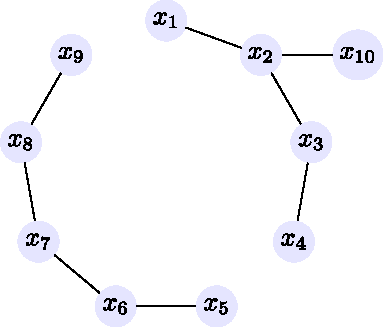
\includegraphics[width=\linewidth]{./images/graph.svg}
\end{image}%
\tcblower
\end{figureptx}%
As one might hope, we do not make \hyperref[x:definition:def-edge-ideal]{Definition~{\xreffont\ref{x:definition:def-edge-ideal}}} merely for fun; given a graph \(G\), it is possible to relate the graph-theoretic properties of \(G\) (e.g., the chromatic number) with the ideal-theoretic properties of \(I(G)\). See \hyperlink{x:biblio:vantuyl-intro}{[{\xreffont 4.1.1}]} and \hyperlink{x:biblio:mfo-waldschmidt}{[{\xreffont 4.1.2}]}, among others, for more.%
%
%
\typeout{************************************************}
\typeout{References 4.1 References}
\typeout{************************************************}
%
\begin{references-subsection-numberless}{References}{}{References}{}{}{g:references:idp105544879968784}
A. Van Tuyl, \emph{\href{http://dx.doi.org/doi:10.1007/978-3-642-38742-5_3}{A Beginner's Guide to Edge and Cover Ideals}\footnote{\nolinkurl{http://dx.doi.org/doi:10.1007/978-3-642-38742-5_3}\label{g:fn:idp105544879970192}}}, in \emph{Monomial Ideals, Computations, and Applications}, Lecture Notes in Mathematics Volume 2083, 2013, pp 63-94C. Bocci, S. Cooper, E. Guardo, et al., \emph{\href{https://doi.org/10.1007/s10801-016-0693-7}{The Waldschmidt constant for squarefree monomial ideals}\footnote{\nolinkurl{https://doi.org/10.1007/s10801-016-0693-7}\label{g:fn:idp105544879971856}}}, \emph{J Algebr Comb} (2016) 44:875\end{references-subsection-numberless}
\end{sectionptx}
%
%
\typeout{************************************************}
\typeout{Section 4.2 Homomorphisms}
\typeout{************************************************}
%
\begin{sectionptx}{Homomorphisms}{}{Homomorphisms}{}{}{x:section:SubSec-Homomorphisms}
\begin{assemblage}{Guiding Questions.}{g:assemblage:idp105544879973776}%
In this section, we'll seek to answer the questions: %
\begin{itemize}[label=\textbullet]
\item{}What is a ring homomorphism?%
\item{}What are some examples of ring homomorphisms?%
\end{itemize}
%
\end{assemblage}
\begin{introduction}{}%
Central to modern mathematics is the notion of \emph{function}\footnote{This section assumes a familiarity with the idea of function from a set-theoretic point of view, as well as the concepts of injective (one-to-one), surjective (onto), and bijective functions (one-to-one correspondences).\label{g:fn:idp105544879976080}}. Functions arise in all areas of mathematics, each subdiscipline concerned with certain types of functions. In algebra, our concern is with \emph{operation-preserving} functions, such as the linear transformations \(L : V\to W\) of vector spaces you have seen in a course in linear algebra. Those linear transformations had the properties that \(L(\mathbf{v}+\mathbf{u}) = L(\mathbf{v})+L(\mathbf{u})\) (addition is preserved) and \(L(c\mathbf{u}) = c L(\mathbf{u})\) (scalar multiplication is preserved).%
\par
We find something similar at work in the study of homomorphisms of rings, which we define to be functions that preserve both addition and multiplication.%
\end{introduction}%
\begin{definition}{}{g:definition:idp105544879978384}%
Let \(R\) and \(S\) be commutative rings with identity. A function \(\p : R\to S\) is a called \terminology{ring homomorphism} if it preserves addition, multiplication, and sends the identity of \(R\) to the identity of \(S\). That is, for all \(x,y\in R\):%
\begin{itemize}[label=\textbullet]
\item{}\(\p(x+y) = \p(x) + \p(y)\),%
\item{}\(\p(xy) = \p(x)\p(y)\), and%
\item{}\(\p(1_R) = 1_S\).%
\end{itemize}
If \(\p\) is a bijection, we say that \(\p\) is an \terminology{isomorphism} and write \(R\cong S\). If \(\p : R\to R\) is an isomorphism, we say \(\p\) is an \terminology{automorphism} of \(R\).%
\end{definition}
Our first job when glimpsing a new concept is to collect a stock of examples.%
\begin{exploration}{}{x:exploration:expl-homomorphism-examples}%
Determine whether the following functions are homomorphisms, isomorphisms, automorphisms, or none of these. Note that \(R\) denotes an arbitrary commutative ring with identity.%
%
\begin{enumerate}
\item{}\(\p : R\to R\) defined by \(\p(x)=x\)%
\item{}\(\psi : R\to R\) defined by \(\psi(x)=-x\)%
\item{}\(\alpha : \Z\to \Z\) defined by \(\alpha(x)=5x\)%
\item{}\(F : \Z_2[x]\to \Z_2[x]\) defined by \(F(p) = p^2\)%
\item{}\(\iota : \C\to \C\) defined by \(\iota(a+bi)=a-bi\), where \(a,b\in \R, i^2 = -1\)%
\item{}\(\beta : \Z\to \Z_{5}\) defined by \(\beta(x) = \overline{x}\)%
\item{}\(\epsilon_r : R[x] \to R\) defined by \(\epsilon_r(p(x)) = p(r)\) (this is known as the \(r\)-evaluation map)%
\item{}\(\xi : \Z_5 \to \Z_{10}\) defined by \(\xi(\overline{x}) = \overline{5x}\)%
\end{enumerate}
\par\smallskip%
\noindent\textbf{\blocktitlefont Solution}.\hypertarget{g:solution:idp105544880060688}{}\quad{}TBD Note that \(\p(x+y) = \overline{x+y} = \overline{x} + \overline{y} = \p(x) + \p(y)\), and similarly for multiplication. We observe that \(\p\) is not an isomorphism, as \(\p(2) = \p(7) = \overline{2}\).%
\end{exploration}%
Homomorphisms give rise to a particularly important class of subsets: kernels.%
\begin{definition}{}{g:definition:idp105544880062608}%
Let \(\p : R \to S\) be a ring homomorphism. Then \(\ker \p =\setof{r\in R}{\p(r)=0_S}\) is the \terminology{kernel} of \(\p\).%
\end{definition}
\begin{activity}{}{g:activity:idp105544880064656}%
For each homomorphism in \hyperref[x:exploration:expl-homomorphism-examples]{Exploration~{\xreffont\ref{x:exploration:expl-homomorphism-examples}}}, find (with justification), the kernel.%
\par\smallskip%
\noindent\textbf{\blocktitlefont Solution}.\hypertarget{g:solution:idp105544880065808}{}\quad{}TBD\end{activity}%
In fact, kernels are not just important subsets of rings; they are ideals.%
\begin{theorem}{}{}{g:theorem:idp105544880066320}%
Given a ring homomorphism \(\p : R\to S\), \(\ker\p\) is an ideal.%
\end{theorem}
\begin{proof}{}{g:proof:idp105544880067600}
If \(x,y\in \ker\p\), \(\p(x+y) = \p(x) + \p(y) = 0_S + 0_S = 0_S\). Similarly, if \(x\in \ker \p\) and \(r\in R\), \(\p(rx) = \p(r) \p(x) = \p(r) 0_S = 0_S\).%
\end{proof}
Kernels also give a useful way of determining whether their defining homomorphisms are one-to-one.%
\begin{theorem}{}{}{g:theorem:idp105544880070160}%
Let \(\p : R\to S\) be a homomorphism. Then \(\p\) is one-to-one if and only if \(\ker\p = \set{0}\).%
\end{theorem}
\begin{proof}{}{g:proof:idp105544880071824}
TBD\end{proof}
\end{sectionptx}
%
%
\typeout{************************************************}
\typeout{Section 4.3 Quotient Rings: New Rings from Old}
\typeout{************************************************}
%
\begin{sectionptx}{Quotient Rings: New Rings from Old}{}{Quotient Rings: New Rings from Old}{}{}{x:section:SubSec-Quotient-Rings}
\begin{assemblage}{Guiding Questions.}{g:assemblage:idp105544880072976}%
In this section, we'll seek to answer the questions: %
\begin{itemize}[label=\textbullet]
\item{}How can we use ideals to build new rings out of old?%
\item{}What sorts of ideals allow us to build domains? Fields?%
\item{}What is the First Isomorphism Theorem?%
\end{itemize}
%
\end{assemblage}
\begin{introduction}{}%
If the only rings that existed were polynomial rings, familiar systems of numbers like \(\Z, \Q, \R, \C\), and matrix rings, there would still be enough to justify the defining the concept of a ring and exploring its properties. However, these are not the only rings that exist. In this section, we explore a way of building new rings from old by means of ideals. To better understand these new rings, we will also define two new classes of ideals: prime ideals, and maximal ideals. We end by briefly connecting these rings to a familiar problem from high school algebra.%
\end{introduction}%
%
%
\typeout{************************************************}
\typeout{Subsection 4.3.1 Congruence modulo \(I\)}
\typeout{************************************************}
%
\begin{subsectionptx}{Congruence modulo \(I\)}{}{Congruence modulo \(I\)}{}{}{g:subsection:idp105544880075664}
The major concept of this section is the notion of congruence modulo \(I\). One can reasonably think of this idea as a generalization of congruence modulo \(m\) in \(\Z\).%
\begin{definition}{}{g:definition:idp105544880078096}%
\index{congruence mod \(I\)}%
Let \(R\) be a ring and \(I\) an ideal of \(R\). Then elements \(a,b\in R\) are said to be \terminology{congruent modulo \(I\)} if \(b-a\in I\). If this is the case, we write \(a + I = b + I\).%
\end{definition}
\begin{activity}{}{g:activity:idp105544880082064}%
Determine (with brief justification) whether \(a + I = b + I\) in the following rings \(R\).%
%
\begin{enumerate}
\item{}\(a = 9\), \(b = 3\), \(I = \ideal{6}\), \(R = \Z\)%
\item{}\(a = 10\), \(b = 4\), \(I = \ideal{7}\), \(R = \Z\)%
\item{}\(a = 9\), \(b = 3\), \(I = \ideal{6}\), \(R = \Z[x]\)%
\item{}\(a = x^2+x-2\), \(b = x-1\), \(I = \ideal{x+1}\), \(R = \Q[x]\)%
\item{}(\emph{Challenge.}) \(a = x^3\), \(b = x^2+2x\), \(I = \ideal{y-x^2, y-x-2}\), \(R = \Q[x,y]\)%
\end{enumerate}
\par\smallskip%
\noindent\textbf{\blocktitlefont Solution}.\hypertarget{g:solution:idp105544880026384}{}\quad{}TBD last one: \(x^3 - x^2 - 2x = x(x-2)(x+1) = -x(y-x^2) + x(y-x-2)\).\end{activity}%
\begin{exploration}{}{g:exploration:idp105544880027024}%
Given a ring \(R\), ideal \(I\), and \(a\in R\), when is it the case that \(a + I = 0 + I = I\)?%
\par\smallskip%
\noindent\textbf{\blocktitlefont Answer}.\hypertarget{g:answer:idp105544880029328}{}\quad{}When \(a\in I\).%
\end{exploration}%
Observe that if \(b-a \in I\), then there is some \(x\in I\) such that \(b-a = x\), and so \(b = a+x\).%
\par
As was the case in \(\Z_m\), congruence modulo \(I\) is an equivalence relation.%
\begin{theorem}{}{}{g:theorem:idp105544880032912}%
Let \(R\) be a ring and \(I\) an ideal of \(R\). Then congruence modulo \(I\) is an equivalence relation on \(R\).%
\end{theorem}
\begin{proof}{}{g:proof:idp105544880035344}
Since \(0\in I\), \(a-a \in I\) for all \(a\), so \(a + I = a+I\) and the relation is reflexive.%
\par
Moreover, if \(b-a \in I\), then \(-1(b-a) = a-b \in I\), so the relation is symmetric.%
\par
If \(b-a \in I\) and \(c-b\in I\), then \((b-a) + (c-b) = c-a \in I\), so the relation is transitive.%
\end{proof}
The set of equivalence classes under this relation is denoted \(R/I\). What is more, this is not merely a set of equivalence classes. As the next two theorems demonstrate, this set possesses two algebraic operations that extend naturally from those of \(R\).%
\begin{theorem}{}{}{x:theorem:thm-addition-mod-I}%
Let \(R\) be a ring and \(I\) an ideal of \(R\). If \(a,b,c,d\in R\) such that \(a+I = b+I\) and \(c+I = d+I\), then \((a+c) + I = (b+d) + I\).%
\end{theorem}
\begin{proof}{}{g:proof:idp105544880044048}
Suppose \(a+I = b+I\) and \(c+I = d+I\). Then \(b-a =x \in I\) and \(d-c = y \in I\). Adding, we have \((b-a) + (d-c) = (b+d) - (a+c) = x+y \in I\). Thus, \((b+d) + I = (a+c) + I\).%
\end{proof}
\begin{theorem}{}{}{x:theorem:thm-multiplication-mod-I}%
Let \(R\) be a ring and \(I\) an ideal of \(R\). If \(a,b,c,d\in R\) such that \(a+I = b+I\) and \(c+I = d+I\), then \(ac + I = bd + I\).%
\end{theorem}
\begin{proof}{}{g:proof:idp105544880050064}
As before, we observe that \(b-a = x\in I\) and \(d-c = y\in I\). Write \(b = x+a\) and \(d = c+y\). Then \(bd = (x+a)(c+y) = xc + xy + ac + ay = ac + \underbrace{(xc+xy+ay)}_{\in I}\), so \(bd - ac \in I\), and thus \(bd + I = ac + I\).%
\end{proof}
The previous two theorems together show that addition and multiplication on the set \(R/I\) is well-defined. As these operations are built on the operations of \(R\), it will likely not surprise you to learn that the usual \hyperref[x:definition:def_ring]{axioms defining a ring} also hold.%
\begin{theorem}{}{}{g:theorem:idp105544880120336}%
\index{quotient ring}%
Let \(R\) be a commutative ring with identity \(1_R\) and \(I\) an ideal of \(R\). The set of equivalence classes modulo \(I\), denoted \(R/I\), is a commutative ring with identity \(1_R + I\) under the operations of addition modulo \(I\) and multiplication modulo \(I\) defined in \hyperref[x:theorem:thm-addition-mod-I]{Theorem~{\xreffont\ref{x:theorem:thm-addition-mod-I}}} and \hyperref[x:theorem:thm-multiplication-mod-I]{Theorem~{\xreffont\ref{x:theorem:thm-multiplication-mod-I}}}.%
\end{theorem}
\begin{proof}{}{g:proof:idp105544880125328}
TBD\end{proof}
Thus, given a ring \(R\) and ideal \(I\) of \(R\), we may build a new ring \(R/I\). In \hyperref[x:subsection:subsec-prime-maximal-ideal]{Subsection~{\xreffont\ref{x:subsection:subsec-prime-maximal-ideal}}}, we will explore the question of when \(R/I\) possesses some of the properties we've previously explored, e.g., when is \(R/I\) a domain? A field? First, we conclude with two explorations. The first gives us a sense of what these rings can look like. The second connects quotient rings to \emph{solution sets} of polynomial equations.%
\begin{exploration}{}{g:exploration:idp105544880128912}%
Consider the ring \(R=\Z_2[x]\) and the ideals \(I = \ideal{x^2-1}\) and \(J = \ideal{x^3 -x -1}\).%
%
\begin{enumerate}
\item{}List the elements of \(R/I\) and \(R/J\).%
\item{}What happens to \(x^2\) in \(R\) when you pass to the quotient ring \(R/I\)? How about \(x^3\) as you pass from \(R\) to \(R/J\)?%
\item{}In view of your answer to the previous question, how does \(x\) behave as you ``mod out'' by \(I\) and \(J\)?%
\item{}Build addition and multiplication tables for each of \(R/I\) and \(R/J\).%
\end{enumerate}
\par\smallskip%
\noindent\textbf{\blocktitlefont Solution}.\hypertarget{g:solution:idp105544880137360}{}\quad{}TBD\end{exploration}%
\begin{exploration}{}{g:exploration:idp105544880137616}%
\index{graph (of a function)}%
\index{zero set}%
One of the most useful connections made in high school algebra is the connection between a function \(f\) (in particular, a polynomial function) and its \emph{graph}. We may extend this notion to ideals via the concept of a \emph{zero set} as follows.%
\par
Let \(F\) be a field and \(R = F[x,y]\) with \(I\subseteq R\) a nonzero ideal. We define the \terminology{zero set} of \(I\), denoted \(Z(I)\), as the set of all points \((a,b)\in F^2\) for which \(f(a,b)=0\) for all \(f\in I\).%
%
\begin{enumerate}
\item{}Suppose \(I = \ideal{f_1, f_2, \ldots, f_n}\). Prove that \((a,b)\in Z(I)\) if and only if \(f_j(a,b) = 0\) for each \(j\in \set{1,\ldots, n}\). Thus, \(Z(I)\) can be determined entirely by examining the generators of \(I\).%
\item{}Describe \(Z(I)\) given \(I = \ideal{y-x^2}\).%
\item{}(Challenge) Given \(I = \ideal{y-x^2}\) and \(J = \ideal{y-x-2}\), describe \(Z(I+J)\) and \(Z(I\cap J)\).%
\item{}Given \(I=\ideal{y-x^2}\), describe the relationship between the variables \(x\) and \(y\) in the quotient \(R/I\). In what way have we restricted our polynomial ``inputs'' to the parabola \(y = x^2\)?%
\end{enumerate}
\par\smallskip%
\noindent\textbf{\blocktitlefont Solution}.\hypertarget{g:solution:idp105544880086288}{}\quad{}TBD.\end{exploration}%
\end{subsectionptx}
%
%
\typeout{************************************************}
\typeout{Subsection 4.3.2 Prime and Maximal Ideals}
\typeout{************************************************}
%
\begin{subsectionptx}{Prime and Maximal Ideals}{}{Prime and Maximal Ideals}{}{}{x:subsection:subsec-prime-maximal-ideal}
In this section, we continue our exploration of quotient rings by looking more closely at properties of ideals. We focus on particular properties of ideals that ensure that the quotient \(R/I\) is either a domain or a field.%
\begin{definition}{}{g:definition:idp105544880088208}%
\index{prime ideal}%
\index{ideal (prime)}%
Let \(R\) be commutative with identity and \(P\subsetneq R\) a nonzero ideal. We say \(P\) is \terminology{prime} if whenever \(a,b\in R\) such that \(ab\in P\), we have \(a\in P\) or \(b\in P\).%
\end{definition}
\begin{theorem}{}{}{g:theorem:idp105544880092304}%
Let \(R\) be a domain and \(p\in R\) be prime. Then \(\ideal{p}\) is a prime ideal.%
\end{theorem}
\begin{proof}{}{g:proof:idp105544880093968}
TBD\end{proof}
\begin{activity}{}{g:activity:idp105544880094224}%
Which of the following ideals are prime?%
\begin{enumerate}
\item{}\(\ideal{9}\) in \(\Z\)%
\item{}\(\ideal{11}\) in \(\Z\)%
\item{}\(\ideal{x^2+1}\) in \(\R[x]\)%
\item{}\(\ideal{x^2-1}\) in \(\R[x]\)%
\item{}\(\ideal{x^2-5x+6, x^4+2x^3-10x^2+5x-2}\) in \(\R[x]\)%
\end{enumerate}
%
\par\smallskip%
\noindent\textbf{\blocktitlefont Solution}.\hypertarget{g:solution:idp105544880102288}{}\quad{}%
\begin{enumerate}
\item{}Not prime. \(3\cdot 3= 9\in \ideal{9}\), but \(3\notin\ideal{9}\).%
\item{}Prime. If \(x\in \ideal{11}\), then \(11|x\) and 11 is prime.%
\item{}Prime. Easy explanation is that \(R[x]/\ideal{x^2+1}\) is isomorphic to \(\C\). \(\ddot\smile\) For now, though, we know that \(x^2+1\) is irreducible, and \(R[x]\) is a PID, so irreducibles are prime.%
\item{}Not prime. \(x^2-1 = (x-1)(x+1)\), but \(x\pm 1\notin \ideal{x^2-1}\) for degree reasons.%
\item{}One may use the EA to show that \(\gcd(x^2-5x+6,x^4+2x^3-10x^2+5x-2) = x-2\), so \(\ideal{x^2-5x+6, x^4+2x^3-10x^2+5x-2} = \ideal{x-2}\). This is prime.%
\end{enumerate}
%
\end{activity}%
It is this precise condition that guarantees that the resulting quotient is a domain.%
\begin{theorem}{}{}{g:theorem:idp105544880111376}%
Let \(R\) be commutative with identity and \(I\) an ideal of \(R\). Then \(I\) is prime if and only if \(R/I\) is an integral domain.%
\end{theorem}
\begin{proof}{}{g:proof:idp105544880113808}
Begin by assuming that \(I\) is prime, and suppose \((a+I)(b+I) = 0+I = I\). Then \(ab \in I\), and since \(I\) is prime, either \(a\in I\) or \(b\in I\). Thus either \(a+I = 0+I\) or \(b+I = 0+I\).%
\par
Now assume that \(R/I\) is a domain. Further, let \(a,b\in R\) be such that \((a+I)(b+I) = ab+I = 0+I\). Then \(ab\in I\), and since \(R/I\) is a domain, \(a+I = 0+I\) or \(b+I = 0+I\), i.e., \(a\in I\) or \(b\in I\). Thus, \(I\) is prime.%
\end{proof}
We now consider another important class of ideals: the maximal ideals.%
\begin{definition}{}{g:definition:idp105544880187152}%
\index{maximal ideal}%
\index{ideal (maximal)}%
Let \(R\) be commutative with identity and let \(M\subsetneq R\) be a nonzero ideal. We say that \(M\) is a \terminology{maximal ideal} if no proper ideal of \(R\) properly contains \(M\). That is, if \(J\) is an ideal satisfying \(M\subseteq J\subseteq R\), either \(J=M\) or \(J=R\).%
\end{definition}
In other words, an ideal \(M\ne R\) is maximal if no ``larger'' ideal (with respect to inclusion) properly contains it. As we will see later, rings can have many maximal ideals.%
\par
It is a fact that any ring \(R\) with \(0_R\ne 1_R\) has a maximal ideal. This follows from \emph{Zorn's Lemma}; a rigorous exploration of Zorn's Lemma lies outside of the scope of this text, but suffice it to say that Zorn's Lemma is incredibly useful in all areas of algebra for proving existence theorems. For example, a proof that every vector space has a basis relies on Zorn's Lemma.%
\par
Rings with only one maximal ideal are said to be \emph{local rings}, and are actively studied in modern research in commutative algebra (the study of commutative rings and their properties).%
\par
The next two results demonstrate that the maximality of \(I\) is precisely the condition that guarantees that \(R/I\) is a field.%
\begin{lemma}{}{}{g:lemma:idp105544880196240}%
Let \(R\) be commutative with identity and \(M\) a maximal ideal of \(R\). Let \(x\in R\setminus M\), and set \(J = \setof{xr+y}{r\in R, \ y\in M}\). Then \(M\subsetneq J\), and thus there exist \(r'\in R\), \(y'\in M\) such that \(1 = xr'+y'\).%
\end{lemma}
\begin{proof}{}{g:proof:idp105544880200208}
TBD\end{proof}
\begin{theorem}{}{}{g:theorem:idp105544880200464}%
Let \(R\) be commutative with identity and \(I\) an ideal of \(R\). Then \(I\) is maximal if and only if \(R/I\) is a field.%
\par\smallskip%
\noindentFor the forward direction, apply the previous lemma to construct an inverse for \(x+I\) given any \(x\in R\setminus I\).%
\end{theorem}
\begin{proof}{}{g:proof:idp105544880204048}
If \(R/I\) is a field, assume \(J\) is an ideal of \(R\) that properly contains \(I\). Let \(x\in J\setminus I\); then \(x+I\) is a nonzero element of \(R/I\), and since \(R/I\) is a field, there is some \(y+I\) such that \((xy)+I = 1+I\). Since \(x\in J\), \(xy\in J\). As \(1+I = (x+I)(y+I) = xy+I\), we have \(1-xy\in I\subsetneq J\), and thus \(1 = (1-xy)+xy \in J\), which means \(J = R\). Thus, \(I\) is maximal.%
\par
Now, suppose that \(I\) is maximal and let \(x\in R\setminus I\). Apply the previous lemma to obtain \(1 = xr' + y'\), where \(y'\in I\). Then%
\begin{equation*}
1 + I = xs+y + I = xs + I = (x+I)(y+I).\qedhere
\end{equation*}
%
\end{proof}
\begin{theorem}{}{}{g:theorem:idp105544880213136}%
Every maximal ideal is prime.%
\end{theorem}
\begin{proof}{}{g:proof:idp105544880213648}
All fields are integral domains. Thus, if \(I\) is maximal, \(R/I\) is a field, thus a domain, and thus \(I\) is prime.%
\end{proof}
In general, the converse is not true (see the \hyperref[x:assemblage:challenge-nonmaximal-prime]{Challenge} below). However, it holds in sufficiently nice rings.%
\begin{theorem}{}{}{x:theorem:thm-pid-primes-are-maximal}%
In a principal ideal domain, every prime ideal is maximal.%
\end{theorem}
\begin{proof}{}{g:proof:idp105544880151184}
Let \(R\) be a PID and \(\ideal{p}\) a prime ideal. By previous work, \(p\) is prime. Suppose that \(\ideal{p} \subseteq \ideal{m}\). Thus, \(p\in \ideal{m}\), so \(m|p\). That is, \(p = mk\). Since \(p\) is prime and \(R\) is a domain, it is irreducible. Thus, either \(m\) or \(k\) is a unit. If \(m\) is a unit, then \(\ideal{m} = R\). If \(k\) is a unit, then \(m = k^{-1} p\), and thus \(m\in \ideal{p}\), which means that \(\ideal{m} = \ideal{p}\).%
\par
Thus, \(\ideal{p}\) is maximal.%
\end{proof}
\begin{exploration}{}{g:exploration:idp105544745503376}%
Describe the prime and maximal ideals of \(\Z\) and \(\Q[x]\).%
\par\smallskip%
\noindent\textbf{\blocktitlefont Hint}.\hypertarget{g:hint:idp105544745504912}{}\quad{}For which ideals \(I\) is \(\Z/I\) a domain? A field? Similarly for \(\Q[x]\). Or, use \hyperref[x:theorem:thm-pid-primes-are-maximal]{Theorem~{\xreffont\ref{x:theorem:thm-pid-primes-are-maximal}}}.\par\smallskip%
\noindent\textbf{\blocktitlefont Solution}.\hypertarget{g:solution:idp105544880166800}{}\quad{}TBD\end{exploration}%
\begin{assemblage}{Challenge.}{x:assemblage:challenge-nonmaximal-prime}%
Find a commutative ring with identity, \(R\), and a nonmaximal prime ideal \(P\) of \(R\).%
\end{assemblage}
\end{subsectionptx}
%
%
\typeout{************************************************}
\typeout{Subsection 4.3.3 Homomorphisms and Quotient Rings}
\typeout{************************************************}
%
\begin{subsectionptx}{Homomorphisms and Quotient Rings}{}{Homomorphisms and Quotient Rings}{}{}{g:subsection:idp105544880171280}
As quotient rings provide fertile soil for building new examples of rings, it should not surprise us to find that homomorphisms interact with quotient rings in interesting and useful ways. Chief among them are the \emph{isomorphism theorems}. In this subsection, we focus primarily on the First Isomorphism Theorem.%
\par
We have seen that any homomorphism \(\p : R\to S\) gives rise to an ideal of \(R\), namely \(\ker\p\). Our next theorem demonstrates that, given a commutative ring with identity \(R\), every ideal is the kernel of some homomorphism defined on \(R\).%
\begin{theorem}{}{}{g:theorem:idp105544880174864}%
Let \(R\) be commutative with identity and \(I\) an ideal of \(R\). Define \(\p: R\to R/I\) by \(\p(r) = r+I\). Then \(\p\) is a homomorphism with \(\ker\p = I\).%
\end{theorem}
In what follows, we work toward a proof of the First Isomorphism Theorem for Rings.%
\par
Throughout, let \(R\) and \(S\) be commutative rings with identity, and let \(\p : R\to S\) be a homomorphism. Recall that \(\im \p = \setof{s\in S}{\p(r) = s\text{ for some } r\in R}\).%
\par
Define \(f: R/\ker \p \to \im \p\) by \(f(r+\ker \p) = \p(r)\).%
\begin{lemma}{}{}{g:lemma:idp105544880181136}%
Using the notation from above, \(f\) is a well-defined function.%
\end{lemma}
\begin{proof}{}{g:proof:idp105544880182032}
Suppose that \(r_1 + \ker\p = r_2 + \ker\p\). Then \(r_2-r_1 \in \ker\p\), so \(\p(r_2-r_1) = 0_S\), and thus \(\p(r_1) = \p(r_2)\). Therefore, \(f(r_1+\ker\p) = f(r_2+\ker\p)\), and \(f\) is well-defined.%
\end{proof}
\begin{lemma}{}{}{g:lemma:idp105544880774544}%
Using the notation above, \(f\) is a homomorphism.%
\end{lemma}
\begin{proof}{}{g:proof:idp105544880775440}
We show that \(f\) preserves addition. That it preserves multiplication will follow similarly. Observe that \(f((x+\ker\p) + (y+\ker\p)) = f((x+y)+\ker\p) = \p(x+y) = \p(x)+\p(y) = f(x+\ker\p) + f(y+\ker\p)\).%
\end{proof}
\begin{lemma}{}{}{g:lemma:idp105544880776592}%
Using the notation above, \(f\) is one-to-one.%
\end{lemma}
\begin{proof}{}{g:proof:idp105544880777488}
Suppose that \(f(r_1 + \ker\p) = f(r_2 + \ker\p)\). That is, \(\p(r_1) = \p(r_2)\). Then \(\p(r_1 - r_2) = 0_S\), so \(r_1 -r_2 \in \ker\p\), and therefore \(r_1 + \ker\p = r_2 + \ker \p\). Thus, \(f\) is one-to-one.%
\end{proof}
\begin{lemma}{}{}{g:lemma:idp105544880780176}%
Using the notation above, \(f\) is onto.%
\end{lemma}
\begin{proof}{}{g:proof:idp105544880781072}
Since \(\p\) is onto \(\im \p\) by definition, given any \(s\in \im \p\) there is some \(r\in R\) such that \(\p(r) = s\). Then \(f(r+\ker\p) = \p(r)\).%
\end{proof}
We thus obtain the following, due to Emmy Noether:%
\begin{theorem}{Noether's Isomorphism Theorem.}{E. Noether}{g:theorem:idp105544880784016}%
\index{First Isomorphism Theorem}%
Let \(\p : R\to S\) be a homomorphism of commutative rings. Then \(R/\ker \p \cong \im \p\).%
\par
In particular, if \(\p : R\to S\) is onto, \(R/\ker \p \cong S\).%
\end{theorem}
The First Isomorphism Theorem gives a useful way of establishing an isomorphism between a quotient ring \(R/I\) and another ring \(S\): find an onto homomorphism \(R\to S\) with kernel \(I\).%
\begin{theorem}{}{}{g:theorem:idp105544880788880}%
We have the following isomorphisms of rings.%
\begin{enumerate}
\item{}\(\displaystyle \Z/\ideal{m} \cong \Z_m\)%
\item{}\(\displaystyle \Q[x]/\ideal{x-5} \cong \Q\)%
\item{}\(\displaystyle \R[x]/\ideal{x^2+1} \cong \C\)%
\end{enumerate}
%
\end{theorem}
\begin{proof}{}{g:proof:idp105544880792720}
TBD Define \(\p: \R[x] \to \C\) by \(\p(p(x)) = p(i)\). We saw earlier that this evaluation map is a homomorphism. It is easy to see that \(\p\) is onto as \(\p(a+bx) = a+bi\) for any \(a,b\in \R\). Thus, \(\R[x]/\ker\p \cong \C\) by the First Isomorphism Theorem.%
\par
We claim that \(\ker\p = \ideal{x^2+1}\). Clearly, \(\ideal{x^2+1} \subseteq \ker\p\). Moreover, \(\ker\p \subsetneq \R[x]\). Finally, \(\ideal{x^2+1}\) is prime and thus maximal, as \(\R[x]\) is a PID. Thus, \(\ker\p = \ideal{x^2+1}\).%
\end{proof}
\begin{activity}{}{g:activity:idp105544880798096}%
Let \(R = \Z_6\) and define \(\p : \Z_6 \to \Z_2\) by \(\p(\overline{x}) = \overline{x}\). That is, \(\p\) sends an equivalence class \(\overline{x}\in \Z_6\) represented by \(x\in \Z\) to the equivalence class represented by \(x\) in \(\Z_2\).%
%
\begin{enumerate}
\item{}Show that \(\p\) is a \hyperref[x:definition:def-well-defined]{well-defined} function.%
\item{}Prove that \(\p\) is a homomorphism.%
\item{}Is \(\p\) onto? Justify.%
\item{}Compute \(\ker\p\) (that is, list the elements in the set). Is \(\p\) one-to-one?%
\item{}Without appealing to the definition, is \(\ker\p\) prime? Maximal? Explain.%
\end{enumerate}
\par\smallskip%
\noindent\textbf{\blocktitlefont Solution}.\hypertarget{g:solution:idp105544880740752}{}\quad{}TBD\end{activity}%
\end{subsectionptx}
\end{sectionptx}
\end{chapterptx}
%
\backmatter%
%
\clearpage\phantomsection%
\addcontentsline{toc}{part}{Back Matter}%
%
%% The index is here, setup is all in preamble
%% Index locators are cross-references, so same font here
{\xreffont\printindex}
%
\end{document}